\documentclass[12pt]{article}
\usepackage[utf8]{inputenc}
\usepackage[english]{babel}

\usepackage{amsthm}
\usepackage{amsmath, amssymb, amsfonts}
\usepackage{mathrsfs}
\usepackage{titling}
\usepackage{hyperref}
\usepackage{url}
\usepackage{bbm}
\usepackage{xcolor}
\usepackage{graphicx}
\graphicspath{ {./Slike/} }
\usepackage{subcaption}
\usepackage{tikz-cd}

\usepackage{geometry}
\geometry{
 a4paper,
 %total={170mm,257mm},
 left=30mm,
 right=30mm,
 top=20mm,
 bottom=20mm
}


\newcommand{\A}{\mathcal{A}}
\newcommand{\B}{\mathcal{B}}
\renewcommand{\AA}{\mathsf{A}}
\newcommand{\BB}{\mathscr{B}}
\newcommand{\BBB}{\mathbb{B}}
\newcommand{\AB}{\mathsf{B}}
\newcommand{\D}{\mathcal{D}}
\renewcommand{\d}{\mathrm{d}}
\newcommand{\E}{\mathsf{E}}
\newcommand{\F}{\mathcal{F}}
\newcommand{\G}{\mathcal{G}}
\renewcommand{\H}{\mathcal{H}}
\newcommand{\Loc}{\mathcal{L}}
\renewcommand{\L}{\mathbb{L}}
\newcommand{\M}{\mathcal{M}}
\newcommand{\MM}{\mathfrak{M}}
\newcommand{\N}{\mathbb{N}}
\newcommand{\NN}{\mathcal{N}}
\renewcommand{\P}{\mathbb{P}}
\newcommand{\PP}{\mathbf{P}}
\newcommand{\Q}{\mathbf{Q}}
\newcommand{\R}{\mathbb{R}}
\newcommand{\RR}{\mathcal{R}}
\renewcommand{\r}{\mathrm{r}}
\newcommand{\Z}{\mathbb{Z}}
\newcommand{\ZZ}{\mathcal{Z}}

\newcommand{\BM}{\mathrm{BM}}
\newcommand{\Law}{\mathrm{Law}}
\newcommand{\Potts}{\mathrm{Potts}}
\newcommand{\TV}{\mathrm{TV}}
\newcommand{\extr}{\mathrm{extr}}

\newcommand{\set}[1]{\left\{#1\right\}}
\newcommand{\oklepaj}[1]{\left(#1\right)}
\newcommand{\oglati}[1]{\left[#1\right]}
\newcommand{\ra}{\rightarrow}
\newcommand{\pika}{\boldsymbol{\cdot}}
\newcommand{\1}{\mathbbm{1}}
\renewcommand{\sp}[1]{\langle #1\rangle}
\newcommand{\ind}{\perp\!\!\!\!\perp}
\renewcommand{\c}{\mathsf{c}}
\newcommand{\supp}{\mathrm{supp}}
\newcommand{\5}{\vspace{0.5cm}}
\renewcommand{\tilde}{\widetilde}
\renewcommand{\hat}{\widehat}

\theoremstyle{definition}
\newtheorem{thm}{Theorem}[section]
\newtheorem{ex}[thm]{Example}
\newtheorem{prop}[thm]{Proposition}
\newtheorem*{sol}{Solution}
\newtheorem*{dis}{Disclaimer}
\newtheorem{df}[thm]{Definition}
\newtheorem{rem}[thm]{Remark}
\newtheorem{lem}[thm]{Lemma}
\newtheorem{cor}[thm]{Corollary}
\newtheorem{conj}[thm]{Conjecture}

\newenvironment{acknowledgements}%
    {\cleardoublepage\thispagestyle{empty}\null\vfill\begin{center}%
    \bfseries Acknowledgements\end{center}}%
    {\vfill\null}

\begin{document}
\pagenumbering{gobble}
\begin{center}
~\\
\vspace{2cm}
\Large{\textbf{Oskar Vavtar}} \\
\vspace{2cm}
\LARGE{\textbf{Absence of Phase Transitions and Preservation of Gibbs Property under Renormalization}} \\
\vspace{3cm}
\large{\textbf{Master thesis\\\vspace{0.2cm} June 25$^?$, 2024}}
\vspace{3cm}\\
\large{\textbf{Supervisor: Dr.~Evgeny A.~Verbitskiy}} \\
\vspace{2cm}

\includegraphics[scale=0.07]{leiden_logo}\\
\large{\textbf{Leiden University\\
Mathematical Institute}}
\end{center}
\pagebreak

% #################################################################################################
% #################################################################################################
% #################################################################################################


\begin{acknowledgements}
\Large{\texttt{Under construction.}}
\iffalse
Firstly, I would like to thank to my supervisor, Evgeny Verbitskiy. You were the first to truly open the world of mathematical statistical mechanics to me, which greatly influenced the way my mathematical tastes developed in the last year. Your guidance during my writing of the thesis allowed me to explore an enormously interesting topic which I could not tackle but myself, while still leaving me enough freedom to figure out things by myself, allowing me to get a little taste of mathematical research. \\

Next, I would like to thank family, my parents Boris and Marjeta, as well as my brothers Filip and Marcel. Not only did you make my study here possible, but supported me throughout the two years and warmly welcomed me back home on my (very frequent) visits. \\

I would also like to thank my friends, both those in Slovenia, who always took time to meet me when I visited home (with a special gratitude to those who managed to visit me here), as well as the new friends I made here. \\

Lastly and with utmost love, I would like to thank to Lana. Your never-ending stream of encouragements, affirmations and love made 
\fi
\end{acknowledgements}
\pagebreak


% #################################################################################################
% #################################################################################################
% #################################################################################################

\pagenumbering{arabic}
\tableofcontents
\pagebreak

% #################################################################################################
% #################################################################################################
% #################################################################################################

\section{Introduction}\label{ch:1}

We begin the introduction by providing some motivation for the theory this thesis explores, which originates in physics. We then proceed to introduce some classical statistical mechanical formalism (which a knowledgeable reader may skip), needed for the rest of the thesis. Lastly, we revisit the motivation presented at the beginning, in a more formal light.

% #################################################################################################

\subsection{Physicist's prologue}

Statistical mechanics of lattice systems is a significant field of modern physics, often overlapping with probability theory, that aims to study macroscopic properties of microscopic systems -- consisting of enormous amounts of non-independent particles -- whose microscopic interactions one can (probabilistically) describe. Much attention has been given to the critical behaviour of those systems, separating the ``stable'' behaviour from ``non-stable'' one, where one vs.~several phases can coexist, as one varies the parameters of the model (such as temperature, magnetic field, etc.). A simple example is a $d$-dimensional Ising model in the absence of the external magnetic field, in which each spin can assume value either $+1$ or $-1$. This allows us to study it as a model on the set of configurations $\set{-1,+1}^{\Lambda}$, where $\Lambda\subseteq\Z^d$. If $\Lambda$ is finite, each configuration $\omega$ can be assigned energy
$$\H(\omega) ~=~ -\beta\sum_{x\sim y}\omega(x)\omega(y),$$
where the sum is over all neighbours in $\Lambda$ (w.r.t.~the nearest-neighbour lattice structure of $\Z^d$) and the quantity $\beta$ represents the inverse temperature. Such function $\H:\set{-1,+1}^{\Lambda}\ra\R$ is called a \textit{Hamiltonian}. Those configurations are assumed to be random and hence one wants to describe their underlying distribution. A key observation is that such physical systems tend to assume configurations with less energy, so a natural choice (also due to some other deeper reasons) of probability distribution is such that each configuration $\omega$ is assigned probability proportional to $\exp(-\H(\omega))$; such measure is defined unambiguously. Problems arise when one wants to consider a similar method for an infinite $\Lambda$, usually $\Z^d$ itself. While one can still obtain a probability measure, that is appropriately consistent with $\H$ in the desired way, the uniqueness of such measure is no longer guaranteed. This is not only a mathematical bug, but reflects very concrete physical properties of the system -- if several consistent probability distributions exist, we say that the system exhibits a phase transition. For example, it has been shown that for the Ising model on $\Z^d$, $d\geq 2$, there is a critical inverse temperature $\beta_c(d)\in(0,\infty)$ so that there's unique such measure for any $\beta<\beta_c(d)$ and several such measures for any $\beta>\beta_c(d)$; for $d=2$, it is known that $\beta_c(2)=\frac{1}{2}\log(1+\sqrt{2})$, while the exact value remains unknown for $d\geq 3$. \\

While the problem of coexistence of several such measures only comes to light in infinite volume, the effects of a high enough $\beta$ already become noticeable in finite volume. In particular, for a high enough $\beta$, the correlations associated with the distribution can be long range (in the sense that they are only bounded through geometry of the volume). This means, that a flip of a spin on an arbitrary location can influence spins on locations arbitrarily far away. This is rather impractical from the physical point of view, as it complicates the analysis of the model at different scales. Despite that, physicists came up with a clever solution on how to deal with this. Instead of considering each spin location $x\in\Lambda$ individually, one partitions $\Lambda$ into $b\times\ldots\times b=b^d$ blocks and considers each of them as one individual super-spin; a block $B$ can be seen as a point in alternative volume $\Lambda'$ (this can be done in several different ways and depends on specifics of the model). Moreover, one defines a ``rule'' $T$, that produces a new configuration $\omega'$, so that for each block $B\in\Lambda'$, $\omega'(B)$ depends (deterministically or stochastically) on $\omega_B=\set{\omega(x):x\in B}$. More formally, $T$ can be seen as a probability kernel $T:\set{-1,+1}^{\Lambda}\times\set{-1,+1}^{\Lambda'}\ra[0,1]$ (see Appendix \ref{app:1}). Below we give some examples of such rules:

\begin{ex}\label{RG:example}
~
\begin{itemize}
	\item[(1)] \textit{Decimation} rule simply forgets all but one of the spin values in $B$, and assigns the value of the one left as the value of the super-spin. In other words, if given $x\in\Z^d$, one has $B_x=\prod_{i=1}^d \set{b x_i,b x_i+1,\ldots,b x_i+(b-1)}=bx+\set{0,\ldots,b-1}^d$, then it is customary to assign
	$$\omega'(B_x) ~=~ \omega(bx).$$
\vspace{-0.9cm}
\begin{figure}[h!]
\centering
\resizebox{0.9\textwidth}{!}{
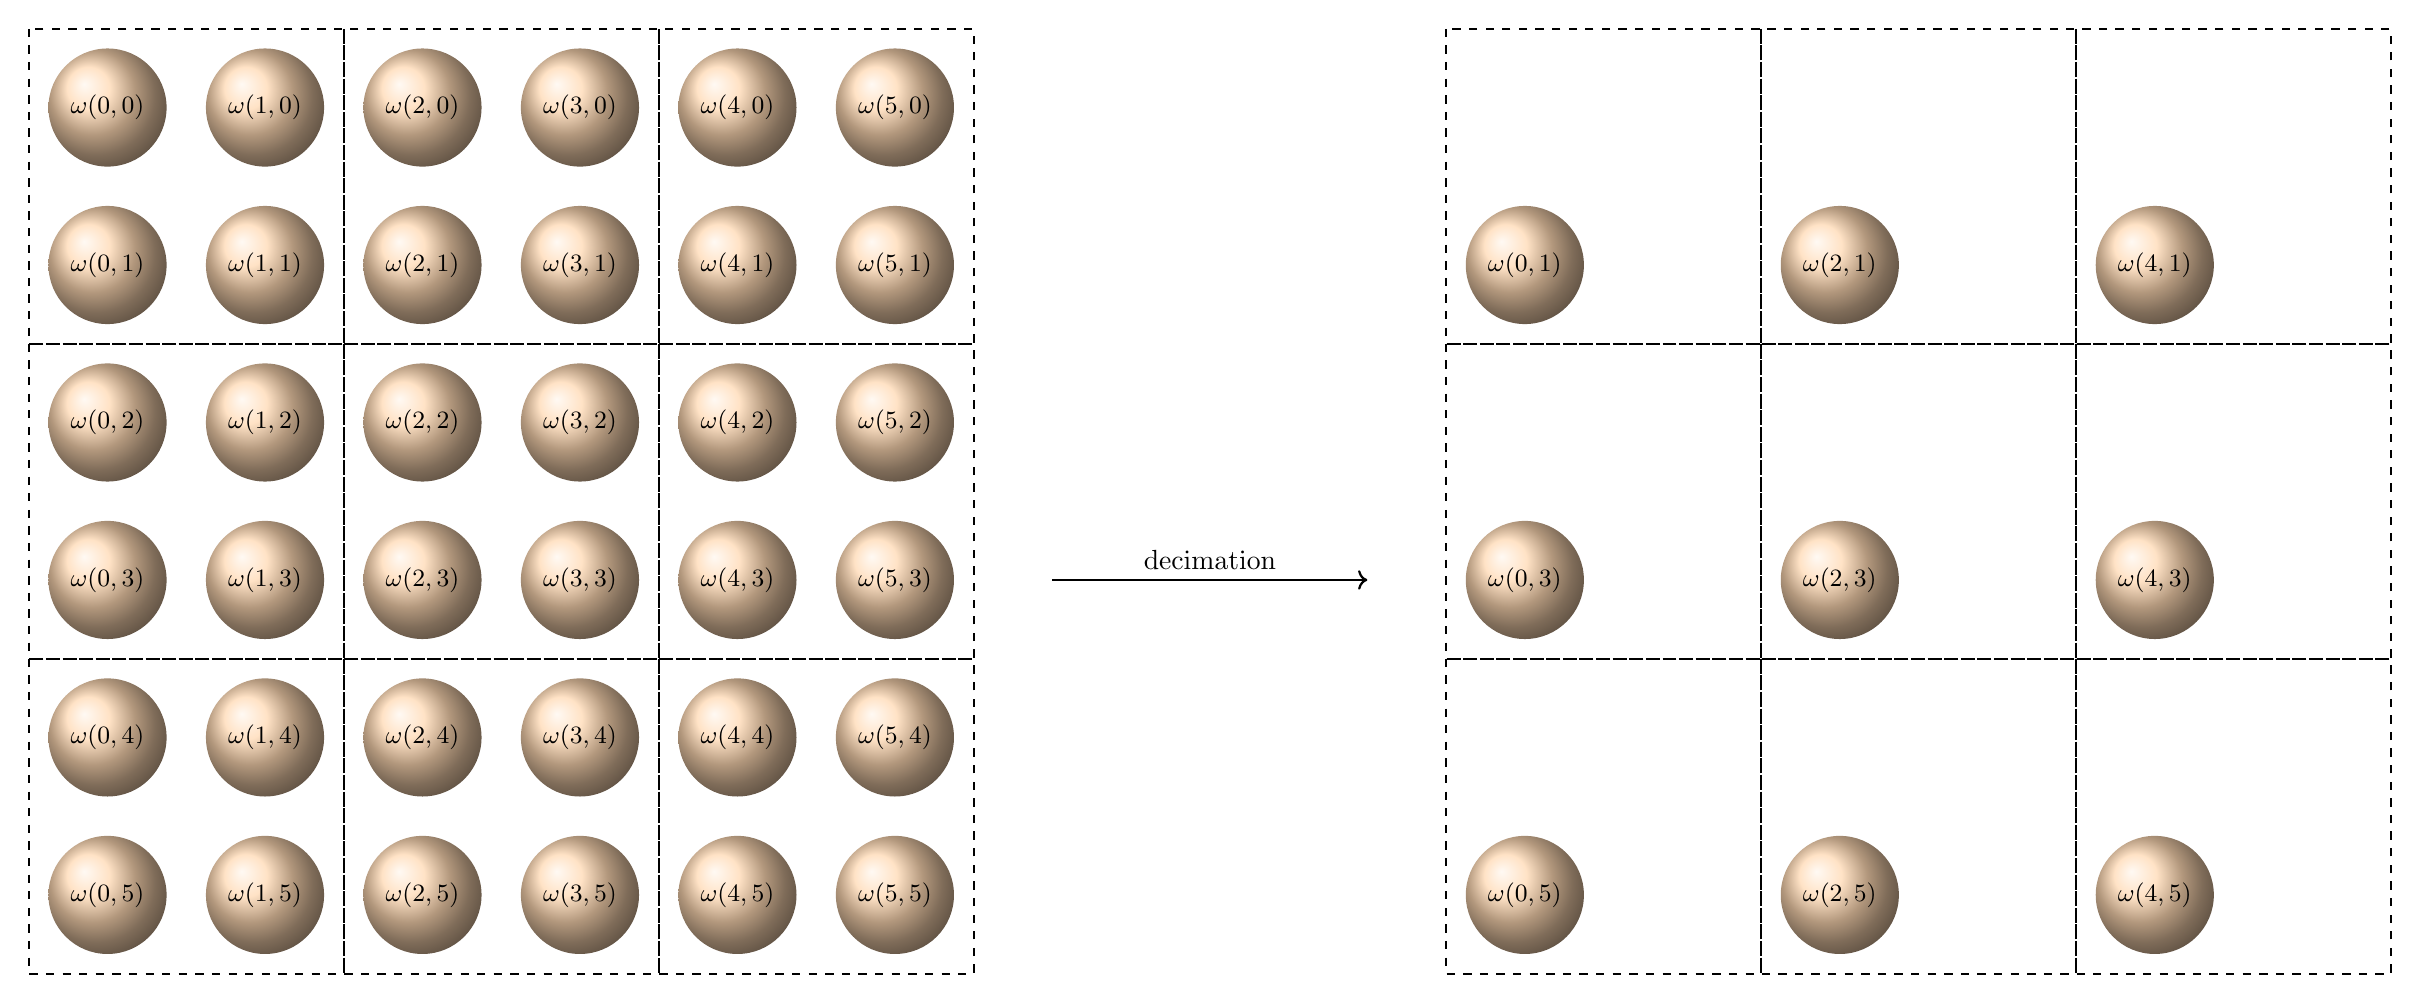
\begin{tikzpicture}
% parameters (?)
\def\spheresize{1.5cm}
\def\spacing{2cm}
% Draw the left grid with labels
    \foreach \i in {0,1,2,3,4,5} {
        \foreach \j in {5,4,3,2,1,0} {
            \node[ball color=orange!30, circle, minimum size=\spheresize] at (\i * \spacing, -\j * \spacing) (x\i\j) {\small $\omega(\i,\j)$};
        }
    }
% Draw the dashed boxes on the left
    \foreach \i in {0,2,4} {
        \foreach \j in {0,2,4} {
            \draw[dashed, thick] (\i*\spacing - \spacing/2, -\j*\spacing + \spacing/2) rectangle (\i*\spacing + 1.5*\spacing, -\j*\spacing - 1.5*\spacing);
        }
    }
% Draw the arrow
    \draw[->, thick] (6*\spacing, -3*\spacing) -- (8*\spacing, -3*\spacing) node[midway, above] {decimation};
% Draw the right grid with labels
    \foreach \i in {0,2,4} {
        \foreach \j in {1,3,5} {
            \node[ball color=orange!30, circle, minimum size=\spheresize] at (9*\spacing + \i * \spacing, -\j * \spacing) (y\i\j) {\small $\omega(\i,\j)$};
        }
    }
% Draw the dashed boxes on the right
    \foreach \i in {0,2,4} {
        \foreach \j in {0,2,4} {
            \draw[dashed, thick] (9*\spacing + \i*\spacing - \spacing/2, -\j*\spacing + \spacing/2) rectangle (9*\spacing + \i*\spacing + 1.5*\spacing, -\j*\spacing - 1.5*\spacing);
        }
    } 
\end{tikzpicture}}
\caption{The illustration of how decimation (with $b=2$) applies in the square lattice. The particles that remain on the right are the ones whose values the corresponding $\omega'(B_x)$'s will assume. The figure is a reproduction of Figure 5.1 in \cite{Ber}.}
\end{figure}
\vspace{-0.5cm}
	\item[(2)] \textit{Majority vote} rule takes into account all the spin values in $B_x$ (defined as above) and assigns it a ``democratically elected'' value; in the case of a draw, a coin is flipped. In other words if $\sum_{y\in B_x}\omega(y)>0$, then $\omega'(B_x)=1$, if $\sum_{y\in B_x}\omega(y)<0$, $\omega'(B_x)=-1$, and if $\sum_{y\in B_x}\omega(y)=0$, $\P(\omega'(B_x)=+1)=\P(\omega'(B_x)=-1)=\frac{1}{2}$. Notice that for boxes of odd size, draws are not possible, so the transformation ceases to be stochastic.
	\item[(3)] \textit{Kadanoff transformation} is in a sense a modification of the majority vote rule, which introduces a notion of ``noise'' in the model and is truly stochastic, regardless, of block size. Given $B_x$ as before and a parameter $\theta>0$, we assign
	$$\omega'(B_x) ~=~ \begin{cases}
	+1, ~&\text{with probability proportional to}~\exp(\theta\sum_{y\in B_x}\omega(y)), \\
	-1, ~&\text{with probability proportional to}~\exp(-\theta\sum_{y\in B_x}\omega(y),
	\end{cases}$$
	independently for each $B_x$. It is clear that in case of a draw, the spin is still decided via a fair coin flip. However, if either $+1$ or $-1$ has more votes, the spin is more likely to be assigned value $\mathrm{sgn}(\sum_{y\in B_x}\omega(y))$, with probability increasing both in $\theta$ and $|\sum_{y\in B_x}\omega(y)|$. One can notice that if we send $\theta\ra\infty$, we recover the majority vote model. Note that due to stochastic properties, this model is already interesting for $B_x=\set{x}$ case.
\end{itemize}
\end{ex}

As one then studies configurations $\omega'$ rather than $\omega$, one should ask questions about their law $\mu'$. In finite volume this can be done in one of two ways:
\begin{itemize}
	\item[(1)] If $\mu$ is the distribution of $\omega$, i.e., $\mu(\omega)\propto\exp(-\H(\omega))$, then one defines
	$$\mu'(\omega') ~:=~ \sum_{\omega\in\set{-1,+1}^\Lambda}T(\omega,\omega')\mu(\omega);$$
	$\mu'$ is then said to be the distribution of $\omega'$. In this sense $T$ defines a map $\mu\mapsto\mu'$ on the space $\M_1(\set{-1,+1}^\Lambda)$.
	\item[(2)] Since $\mu$ is derived from $\H$, one should want to obtain $\mu'$ in a similar way, by finding an appropriate Hamiltonian $\H'$ and put $\mu'(\omega')\propto\exp(-\H'(\omega'))$. In particular $\H'$ is taken such that
	$$\exp(-\H(\omega')) ~=~ \sum_{\omega\in\set{-1,+1}^{\Lambda}}T(\omega,\omega')\exp(-\H'(\omega')).$$
	If this can be done unambiguously, we obtain a map $\H\mapsto\H'$, which we denote by $\RR$.
\end{itemize}

As soon as one has maps between $\mu$, $\mu'$, $\H$ and $\H'$ well defined, one can switch working between Hamiltonians and associated measures, as suggested by the diagram below:
\begin{equation}\label{RGdiagram}
\begin{tikzcd}
    \H \arrow[r, mapsto, "\RR"] \arrow[d, mapsto] & \H' \\
    \mu \arrow[r, mapsto, "T"] & \mu' \arrow[u, mapsto]
\end{tikzcd}
\end{equation}

As the infinite volume case is plagued with at least as much technical difficulties as the finite volume one, one might want to use a similar technique on the general $\Z^d$ lattice. However, the situation does not remain as straightforward as in the setting described above: one can no longer freely switch between working with Hamiltonians and associated measures. First obvious issue is the possible coexistence of several infinite volume measures $\mu$ consistent with $\H$; in this case, the map $\H\mapsto\mu$ is multi-valued. Despite this, one can still formally define the map $\mu\mapsto\mu'$, to which we will return later. \\

Having obtained $\mu'$, one ``should'' then be able to recover an appropriate Hamiltonian $\H'$, with which $\mu'$ is consistent; At least, that was believed by physicists for a long time. In particular, it was assumed that for any image measure $\mu'$ (under $T$), there exists an appropriate Hamiltonian with which $\mu'$ is consistent, so that the map $\mu'\mapsto\H'$ is well defined (and hence $\H\mapsto\H'$). This assumption was challenged in the late 70's and early 80's by Israel in \cite{Isr} as well as Griffiths and Pearce in \cite{GP1},\cite{GP2},\cite{Grif}. In the early 90's, van Enter, Fern\'andez and Sokal rigorously demonstrated in \cite{EFS} that such assumption is false in many famous examples and provided a rigorous framework to address pathologies related to RG maps. This included a conjecture about the equivalent conditions for well-posedness of $\H\mapsto\H'$. \\

It is precisely this conjecture that is central to this thesis. Before we continue any further, we introduce some formal background one should be equipped with when studying statistical mechanics of lattice systems. We then conclude this introductory chapter, by revisiting the basics of renormalization in a more formal light.

% #################################################################################################

\subsection{Preliminaries: interactions, Hamiltonians and Gibbs measures}

As mentioned before, the central aim of statistical mechanics is to provide a probabilistic description of microscopic physical phenomena. In particular one aims to study a collection of particles (often infinite), indexed in some lattice $\L$ and each taking values in some set $\A_x$, $x\in\L$, called the \textit{(single-)spin space}, which we will assume to be finite.\footnote{In general, one can take $\A$ to be infinite, even uncountable (e.g., $\R^d$).} Each manifestation of this macroscopic system corresponds to a (random) configuration in $\Omega=\prod_{x\in\L}\A_x$; often we will assume that the system is homogeneous, i.e., $\Omega=\A^{\L}$. In order to talk about randomness, we have to consider probability distributions on $\Omega$; we will write $\M_1(\Omega)$ for the set of probability measures on $\Omega$ (or rather $(\Omega,\F)$, where $\F$ is the  corresponding $\sigma$-algebra, generated by cylinder sets). One often calls those measures \textit{random fields}. \\

There is however a particular class of probability measures that are of interest, called \textit{Gibbs measures}, which we will start introducing formally in a moment, but not before giving some intuitive but \textit{very} informal description. Generally, we assume that the particles interact in some sense, which contributes some (positive or negative) energy. If some configuration $\omega$ carries energy $\H(\omega)$, then the Gibbs measure (consistent with $\H$) would assign $\omega$ a probability proportional to $\exp(-\H(\omega))$. Intuitively, Gibbs measures award configurations with low energy and penalize configurations with high energy. 

% *************************************************************************************************

\subsubsection{Formal definition, part 1: finite volume setting}\label{FiniteVolumeSetting}

In this section we assume $|\L|<\infty$; an often used example would be a finite graph $G=(V,E)$. In order to capture the interactions, one defines a collection of maps $\Phi=\set{\Phi_\Lambda:\Lambda\subseteq\L}$, called \textit{interaction}, where for $\omega\in\Omega$, $\Phi_\Lambda(\omega)$, depends on $\omega$ only through its values in $\Lambda$, that is, $\Phi_\Lambda(\omega)=\Phi_\Lambda(\omega(x)\!:\!x\in\Lambda)$. The value $\Phi_\Lambda(\omega)$ represents the amount of energy that the interaction between particles in $\Lambda$ contributes to the system.

\begin{ex}
Often studied are the \textit{nearest-neighbour} interactions. If $\L$ is a (not necessarily finite) graph $G=(V,E)$, then $\Phi_\Lambda$ is constant zero, unless $\Lambda=\set{x,y}$, where $x\sim y$, or $\Lambda=\set{x}$.
\end{ex}

The total energy of the systems is then obtained by summing up energies of all subsets:
$$\H(\omega) ~=~ \sum_{\Lambda\subseteq \L}\Phi_\Lambda(\omega), \quad \omega\in\Omega.$$
We call the function $\H=\H^\Phi$ a \textit{Hamiltonian} consistent with $\Phi$. As already suggested above, the Gibbs measure $\mu=\mu^\Phi$ is then defined as
$$\mu(\omega) ~=~ \frac{1}{\ZZ}\exp(-\H(\omega)), \quad \omega\in\Omega,$$
where $\ZZ=\ZZ^\Phi$ is called the \textit{partition function} and is given by $\ZZ ~=~ \sum_{\omega\in\Omega}\exp(-\H(\omega)).$ In this finite volume setting, Gibbs measures also often called \textit{Gibbs canonical ensembles.} \\

While from probabilistic point of view, this may be interesting enough model, it is rather limiting from the statistical mechanical point of view. In particular, there are no phase transitions, i.e., coexistence of several Gibbs measure consistent with the same interaction, which is one of the main focuses of study in statistical mechanics. This does, however, change when we relax the assumption about finiteness of $\L$ and take it to be a countably infinite lattice, as we will see shortly.

% *************************************************************************************************

\subsubsection{Formal definition, part 2: infinite volume setting}

In practice, one often wishes to consider $\L$ to be an infinite lattice. Unfortunately, the construction presented in the previous section does not translate to this setting, as the Hamiltonian would correspond to an infinite sum and hence the Gibbs measure generally would not be well defined. We thus have to consider an alternative construction of Gibbs measures in infinite volumes. The most intuitive approach perhaps appears to be to construct them as (weak) limits of measures from the previous section, as finite volumes increase to $\L$ in a suitable sense. This indeed is a valid idea: one can construct infinite-volume Gibbs measures in this way and those measures form an import class. However, it is not the entire story. We will now proceed to define (repeating some already mentioned notions) a more general notion of infinite-volume Gibbs measures, which includes all such limit measures as well as other ones. \\

From now on we restrict ourselves to $\L=\Z^d$. In the rest of the thesis, we will only consider $\L$ to be either $\Z^d$ or some subset of it. Moreover, given $\omega\in\Omega$ and $\Lambda\subseteq\Z^d$, we write $\omega_\Lambda:=\omega|_\Lambda$ as well as $\Omega_\Lambda:=\prod_{x\in\Lambda}\A_x$, so that $\omega_\Lambda\in\Omega_\Lambda$, and $\F_\Lambda$ for the (corresponding) $\sigma$-algebra on $\Omega_\Lambda$, generated by the cylinders on subsets of $\Lambda$.\footnote{The advantage of directly selecting $\omega_\Lambda$ from $\Omega_\Lambda$, rather than $\omega$ from $\Omega$ and just restricting it, is that for $\Lambda\Subset\Z^d$ one has $|\Omega_\Lambda|<\infty$, which allows for finite sums.} Also, given another $\tilde{\omega}\in\Omega$, we denote by $\omega_\Lambda\tilde{\omega}_{\Lambda^\c}$ a configurations such that
$$[\omega_\Lambda\tilde{\omega}_{\Lambda^\c}](x) ~:=~ \begin{cases}
\omega(x): ~&x\in\Lambda,\\
\tilde{\omega}(x): ~&x\in\Lambda^\c.
\end{cases}$$

\begin{df}~
\begin{itemize}
	\item[(1)] An \textit{interaction} is a collection of maps $\Phi=\{\Phi_\Lambda:\Lambda\Subset\Z^d\}$, such that for each $\Lambda\Subset\Z^d$,
$$\Phi_\Lambda(\omega) ~=~ \Phi_\Lambda(\omega_\Lambda), \quad \forall\omega\in\Omega,$$
that is, $\Phi_\Lambda$ depends on $\omega$ only through its values in $\Lambda$. We say that $\Phi$ is \textit{uniformly absolutely convergent} (UAC) if 
$$\|\Phi\| ~:=~ \sup_{x\in\Z^d}\sum_{\substack{\Lambda\Subset\Z^d:\\x\in\Z^d}}\|\Phi_\Lambda\|_\infty ~<~ \infty$$
and write $\BB^1(\Omega)$ for the collection of all UAC interactions on $\Omega$.
	\item[(2)] For $\Phi\in\BB^1(\Omega)$, we define a corresponding collection of Hamiltonians $\H^\Phi=\set{\H_\Lambda^\Phi:\Lambda\Subset\Z^d}$, given by
	$$\H_\Lambda^\Phi(\omega) ~=~ \sum_{\substack{\Delta\Subset\Z^d:\\\Delta\cap\Lambda\neq\emptyset}}\Phi_\Delta(\omega), \quad \omega\in\Omega.$$
	\item[(3)] For $\Phi\in\BB^1(\Omega)$, we define a \textit{specification} as a collection $\gamma^\Phi=\set{\gamma_\Lambda^\Phi:\Lambda\Subset\Z^d}$ via
	$$\gamma_\Lambda^\Phi(\tilde{\omega}_\Lambda|\omega_{\Lambda^\c}) ~=~ \frac{1}{\ZZ_\Lambda^{\Phi,\omega}}\exp(-\H_\Lambda^\Phi(\tilde{\omega}_\Lambda\omega_{\Lambda^\c})), \quad \omega,\tilde{\omega}\in\Omega,$$
	where $\ZZ_\Lambda^{\Phi,\omega}=\sum_{\tilde{\omega}_\Lambda\in\Omega_\Lambda}\exp(-\H_\Lambda^\Phi(\tilde{\omega}_\Lambda\omega_{\Lambda^\c}))$.
\end{itemize}
\end{df}

\begin{rem}\label{rem:specification}
Formally, $\gamma^\Phi$ should be seen as a collection of probability kernels, where for each $\Lambda\Subset\Z^d$, $\gamma_\Lambda^\Phi:\F_\Lambda\times\Omega_{\Lambda^\c}\ra(0,1)$, so $\gamma_\Lambda^\Phi(\tilde{\omega}_\Lambda|\omega_{\Lambda^\c})$ should be actually read as $\gamma_\Lambda^{\Phi}(\set{\tilde{\omega}_\Lambda}|\omega_{\Lambda^\c})$. The probability of a general $A\in\F_\Lambda$ is now given by
$$\gamma_\Lambda^\Phi(A|\omega_{\Lambda^\c}) ~=~ \sum_{\tilde{\omega}_\Lambda\in A}\gamma_\Lambda^\Phi(\tilde{\omega}_\Lambda|\omega_{\Lambda^\c}).$$
The corresponding expectation is given for suitable $f:\Omega\ra\R$ by
$$\gamma_\Lambda^\Phi[f|\omega_{\Lambda^\c}] ~=~ \sum_{\tilde{\omega}_\Lambda\in\Omega_\Lambda}f(\tilde{\omega}_\Lambda\omega_{\Lambda^\c})\gamma_{\Lambda}^\Phi(\tilde{\omega}_\Lambda|\omega_{\Lambda^\c}).$$
In further generality, we may call \textit{a specification} any collection of probability kernels $\gamma=\set{\gamma_\Lambda:\Lambda\Subset\Z^d}$ such that for each $\Lambda\Subset\Z^d$
\begin{itemize}
	\item and  $A\in\F_{\Lambda}$, $\omega\mapsto\gamma(A|\omega)$ is $\F_{\Lambda^\c}$-measurable,
	\item $\gamma_\Lambda(A|\pika)=\1_A$ for each $A\in\F_{\Lambda^\c}$,
	\item and $\Delta\subset\Lambda$, $\int \gamma_\Delta(A|\omega')\,\gamma_\Lambda(\d\omega'|\omega)=\gamma_\Lambda(A|\omega)$.
\end{itemize}
\end{rem}

Finally, after introducing all these notions, we are able to formally define the infinite-volume Gibbs measures, using a very natural definition.

\begin{df}[Infinite volume DLR-Gibbs measure]\label{def:DLR}
A probability measure $\mu\in\M_1(\Omega)$ is said to be a Gibbs measure consistent with $\Phi\in\BB^1(\Omega)$, if it is consistent with $\gamma^\Phi$, that is, if for each $\Lambda\Subset\Z^d$ we have
$$\mu(\omega_\Lambda|\omega_{\Lambda^\c}) ~=~ \gamma_\Lambda^\Phi(\omega_\Lambda|\omega_{\Lambda^\c}) \quad~\text{for}~\mu\text{-a.a.}~\omega\in\Omega.\footnote{The notation $\mu(a_\Lambda|b_{\Lambda^\c})$ should be read as $\mu(a~\text{on}~\Lambda|b~\text{off}~\Lambda)$.}$$
We write $\G_\Omega(\Phi)$ for the set of all Gibbs measure on $\Omega$ consistent with $\Phi$. Alternatively, if our main reference is a specification $\gamma$ or a collection of Hamiltonians $\H$, we may also write $\G_\Omega(\gamma)$ or $\G_\Omega(\H)$, so in our notation $\G_\Omega(\Phi)$, $\G_\Omega(\H^\Phi)$ and $\G_\Omega(\gamma^\Phi)$ would refer to the same thing.
\end{df}

\begin{rem}\label{Rem:DLR}
~
\begin{itemize}
	\item[(i)] Equivalently, one could define $\mu$ to be Gibbs w.r.t.~specification $\gamma$ if for each $\Lambda\Subset\Z^d$ and $f\in C(\Omega)$ one has
	$$\int f\,\d\mu ~=~ \int\gamma_\Lambda[f|\omega_{\Lambda^\c}]\,\d\mu(\omega).$$
	\item[(ii)] For each $\Phi\in\BB^1(\Omega)$, $\G_\Omega(\Phi)\neq\emptyset$.
\end{itemize}
\end{rem}

\begin{ex}[Ising model]
One of the most classical models in statistical mechanics is the Ising model, concerned with (ferro)magnetism. It is an example of a nearest-neighbour model with $\A=\set{-1,+1}$, where the Hamiltonian corresponding to a finite volume $\Lambda\Subset\Z^d$ is given by
$$\H_{\Lambda;\beta,h}(\omega) ~=~ -\beta\!\!\!\!\!\!\!\sum_{\substack{x\sim y:\\x\in\Lambda~\text{or}~y\in\Lambda\\}}\!\!\!\!\!\!\!\omega(x)\omega(y) + h\sum_{x\in\Lambda}\omega(x),$$
though one often writes ``$2\1_{\set{\omega(x)=\omega(y)}}-1$'' instead of ``$\omega(x)\omega(y)$'', as the latter ceases to be suitable in case one chooses an alternative $\A$ (such as $\set{0,1}$ for example). The parameters $\beta\geq 0$ and $h\in\R$ represent the \textit{inverse temperature} and the \textit{external field}, respectively. Thus, considering a boundary condition $\xi\in\Omega$, the probability of configuration agreeing with $\omega$ on $\Lambda$, conditional on it agreeing with $\xi$ outside $\Lambda^c$, given by
$$\gamma_{\Lambda;\beta,h}(\omega_\Lambda|\xi_{\Lambda^\c}) ~=~ \frac{1}{\ZZ_{\Lambda;\beta,h}^\xi}\exp(-\H_{\Lambda;\beta,h}(\omega_\Lambda\xi_{\Lambda^\c})),$$
where $\ZZ_{\Lambda;\beta,h}^\xi=\sum_{\tilde{\omega}_\Lambda\in\Omega_\Lambda}\exp(-\H_{\Lambda;\beta,h}(\tilde{\omega}_\Lambda\xi_{\Lambda^\c}))$, only depends on the boundary condition through vertices that are adjacent to some vertex in $\Lambda$, i.e., are touching the boundary. This is in fact a general property of nearest-neighbour models.
\end{ex}

Very important is the following characterization of Gibbs measures, which is often used to prove Gibbsianity of concrete measures.
\begin{prop}\label{DLR:equiv}
~
\begin{itemize}
	\item[(i)] Let $\Phi\in\BB^1(\Omega)$. Then $\gamma^\Phi$ has the following two properties:
		\begin{itemize}
			\item \textit{uniform non-nullness}: for every $\Lambda\Subset\Z^d$ there exist $\alpha_\Lambda,\beta_\Lambda\in(0,1)$ such that
			$$\alpha_\Lambda ~\leq~ \gamma_\Lambda^\Phi(\tilde{\omega}_\Lambda|\omega_{\Lambda^\c}) ~\leq~ \beta_\Lambda, \quad\forall\omega,\tilde{\omega}\in\Omega.$$
			\item \textit{quasilocality}: writing $\BBB_n=[-n,n]^d\cap\Z^d$ for $n\in\N$, for every $\Lambda\Subset\Z^d$ one has
			$$\sup_{\omega,\tilde{\omega}\in\Omega}\sup_{\xi,\zeta\in\Omega}|\gamma_\Lambda^\Phi(\tilde{\omega}_\Lambda|\omega_{\BBB_n\setminus\Lambda}\xi_{\BBB_n^\c\setminus\Lambda})-\gamma_\Lambda^\Phi(\tilde{\omega}_\Lambda|\omega_{\BBB_n\setminus\Lambda}\zeta_{\BBB_n^\c\setminus\Lambda})| ~\xrightarrow{n\ra\infty}~ 0.$$
		\end{itemize}
		\item[(ii)] Let $\mu$ be a fully supported Borel probability measure on $\Omega$. If there exists a specification (in the sense of Remark \ref{rem:specification}) which is uniformly non-null, quasilocal and with which $\mu$ is consistent (in the sense of Definition \ref{def:DLR}/Remark \ref{Rem:DLR}), then there exists some $\Phi\in\BB^1(\Omega)$ so that $\mu\in\G_\Omega(\Phi)$.
		
\end{itemize}
\end{prop}

% *************************************************************************************************

\subsubsection{Coexistence of several Gibbs measures}

While the Remark \ref{Rem:DLR}.(ii) tells us that for an UAC interaction, there always exists at least one Gibbs measure, it tells us nothing else about the cardinality in $\G_\Omega(\Phi)$: in particular it doesn't guarantee that there's only one. In fact several Gibbs measures consistent with the same interaction may exist. In this case, we say that the system has a \textit{phase transition}. Given a model with some parameter(s), an important question is for which parameter values there is only one Gibbs measure and for which parameter values there are several. \\

We begin by introducing the most intuitive method of defining infinite volume Gibbs measure, which was already hinted on earlier, using the weak limits. Gibbs measures obtained in this way are often referred to as \textit{thermodynamic limits (of finite volume Gibbs measures)}. Despite definition being straightforward, it requires us to first introduce some technical notions, which will be used throughout the thesis:

\begin{df}
~
\begin{itemize}
	\item[(1)] We say that $(\Lambda_n)_{n\in\N}$, where $\Lambda_n\Subset\Z^d$ for each $n\in\N$, is a \textit{van Hove sequence}, if it satisfies the following conditions:
	\begin{itemize}
		\item[(i)] it is \textit{increasing}: $\Lambda_n\subset\Lambda_{n+1}$ for each $n\in\N$,
		\item[(ii)] it \textit{invades} $\Z^d$: $\bigcup_{n\geq 1}\Lambda_n=\Z^d$, and
		\item[(iii)] $\lim_{n\ra\infty}\frac{|\partial\Lambda_n|}{|\Lambda_n|}=0$, where $\partial \Lambda=\set{x\in\Lambda^\c:\exists y\in\Lambda,x\sim y}$.
	\end{itemize}
	We denote van Hove convergence by $\Lambda_n\Uparrow\Z^d$.
	\item[(2)] A function $f:\Omega\ra\R$ is said to be \textit{local} if there's $\Delta\Subset\Z^d$, such that for any choice of $\omega,\tilde{\omega}\in\Omega$, 
	$$\omega(x)=\tilde{\omega}(x)~\forall x\in\Delta ~\Longrightarrow~ f(\omega)=f(\tilde{\omega}).$$
	We sometimes write $\supp(f)$ (or by abuse of notation, $\D_f$) for the minimal such $\Delta$. We denote the collection of all local functions $f:\Omega\ra\R$ by $\Loc(\Omega)$.
	\item[(c)] Given (probability) measures $\mu,\mu_1,\mu_2,\ldots$ on $\Omega$, we say that $(\mu_n)_{n\in\N}$ converges \textit{weakly} to $\mu$, writing $\mu_n\xrightarrow{w}\mu$, if
	$$\int_\Omega f\,\d\mu_n ~\ra~ \int_\Omega f\,\d\mu, \quad \forall f\in\Loc(\Omega).$$
\end{itemize}
\end{df}

The definitions then goes as follows:

\begin{df}[Thermodynamic-limit Gibbs measure]
We say that $\mu$ is a thermo\-dynamic-limit Gibbs measure for $\Phi\in\BB^1(\Omega)$, if there exists a boundary condition $\xi\in\Omega$, such that
$$\gamma_{\Lambda_n}^\Phi(\pika|\xi_{\Lambda^\c}) ~\xrightarrow{w}~ \mu \quad \text{as}~n\ra\infty,$$
for arbitrary van Hove sequence $(\Lambda_n)_{n\in\N}$.
\end{df}

\begin{rem}\label{rem:InfVol}
The notation in the above definition is slightly dishonest, in terms of what $\gamma_\Lambda^\Phi$ is supposed to represent, though conceptually is ``correct enough'' to allow for the abuse of notation. While ``$\mu_n$'' is supposed to be a probability measure on $\Omega$, we have seen that given $\Lambda\Subset\Z^d$ and $\xi\in\Omega$ fixed, $\gamma_\Lambda^\Phi(\pika|\xi_{\Lambda^\c})$ is a probability measure on $\Omega_\Lambda$, so one could argue that the weak limit in the above definition technically speaking does not make sense. The formal way to correct it would be to define, for each $\Lambda\Subset\Z^d$ and $\xi\in\Omega$ a measure $\mu_\Lambda^\xi=\mu_\Lambda^{\Phi,\xi}$ given by
$$\mu_\Lambda^\xi(\omega) ~=~ \1_{\set{\omega_{\Lambda^\c}=\xi_{\Lambda^\c}}}\gamma_\Lambda^\Phi(\omega_\Lambda|\xi_{\Lambda^\c}), \quad \omega\in\Omega,$$
which is indeed a probability measure on $\Omega$ (while still in a sense ``supported'' on $\Omega_\Lambda$, in the sense that $\supp(\mu_\Lambda^\xi)=\Omega_\Lambda\times\set{\xi_{\Lambda^\c}}$), so the weak limit in the definition above indeed makes sense.
\end{rem}

\begin{ex}[Ising: $+$ and $-$ phases]
Simple examples of thermodynamic limits are the so-called $+$ and $-$ states in the Ising model. First, we define, for $\beta>0$, $h\in\R$, $\Lambda\Subset\Z^d$ and $\xi\in\Omega$,
$$\mu_{\Lambda;\beta,h}^\xi(\omega) ~=~ \1_{\set{\omega_{\Lambda^\c}=\xi_{\Lambda^\c}}}\frac{1}{\ZZ_{\Lambda;\beta,h}^\xi}\exp(-\H_{\Lambda;\beta,h}(\omega_\Lambda\xi_{\Lambda^\c})), \quad \omega\in\Omega.$$
Thermodynamic limits $\mu_{\beta,h}^{+}$ and $\mu_{\beta,h}^{-}$ are obtained as 
$$\mu_{\BBB_n;\beta,h}^+\xrightarrow{w}\mu_{\beta,h}^+ \quad\text{and}\quad \mu_{\BBB_n;\beta,h}^-\xrightarrow{w}\mu_{\beta,h}^-,$$
where $+$ is constant $+1$ and $-$ is constant $-1$. An important question is whether those limits coincide, i.e., if $\mu_{\beta,h}^+=\mu_{\beta,h}^-$ as members of $\M_1(\Omega)$. For $h\neq 0$, the answer is \textit{yes}. However, for $h=0$ and $d\geq 2$, this is no longer the case. For each dimension $d\geq 2$, there exists a critical inverse temperature $\beta_c=\beta_c(d)\in(0,\infty)$ such that for $\beta<\beta_c$ we have $\mu_{\beta,0}^+=\mu_{\beta,0}^-$ (and in fact $|\G_\Omega(\Phi_{\beta,0})|=1$) while for $\beta>\beta_c$ we have $\mu_{\beta,0}^+\neq\mu_{\beta,0}^-$ (so $|\G_{\Omega}(\Phi_{\beta,0})|>1$).
\end{ex}

We now turn our attention to the general notion on Gibbs measures, as defined in Definition \ref{def:DLR}, which are often referred to as the \textit{DLR Gibbs measures}, named after Dobrushin, Lanford and Ruelle. Spaces of DLR Gibbs measures (from now on just Gibbs measures) do indeed carry some nice properties:

\begin{prop}\label{DLR:properties}
Let $\Phi\in\BB^1(\Omega)$. Then:
\begin{itemize}
	\item[(i)] $\G_\Omega(\Phi)$ is convex.
	\item[(ii)] Extremal measures of $\G_\Omega(\Phi)$ (denoted by $\extr(\G_\Omega(\Phi))$) are mutually singular.
	\item[(iii)] For each $\mu\in\extr(\G_\Omega(\Phi))$,
	$$\gamma_{\BBB_n}^\Phi(\pika|\omega) ~\xrightarrow{w}~ \mu, \quad \text{for}~\mu\text{-a.a.}~\omega\in\Omega,$$
	keeping in mind Remark \ref{rem:InfVol}. In other words, extremal $\mu$ can be obtained as a thermodynamic limit with some fixed boundary condition.
\end{itemize}
\end{prop}

\begin{ex}[Ising: +/- vs.~Dobrushin]
In the case of Ising model in the non-uniqueness regime (that is, $d\geq 2$, $h=0$ and $\beta>\beta_c(d)$), the thermodynamic limits corresponding to boundary conditions $+$ and $-$ are both extremal Gibbs measures -- in fact, they are the only ones:
$$\mathrm{extr}(\G_\Omega(\Phi_{\beta,h})) ~=~ \set{\mu_{\beta,0}^+,\mu_{\beta,0}^-}.$$
An interesting example of a non-extremal boundary condition is the \textit{Dobrushin boundary condition}, which is given by
$$\mathrm{Dob}(x) ~=~ \begin{cases}
+1: ~&x=(x_1,\ldots,x_d)~\text{with}~x_d\geq 0,\\
-1: ~&\text{otherwise}. 
\end{cases}$$
While $\mu_{\beta,0}^{\mathrm{Dob}}\notin\mathrm{extr}(\G_\Omega(\Phi_{\beta,0}))$, it can still be obtained by a thermodynamical limit (and is a well-defined Gibbs measure), see \cite{FV}, Theorem 3.58. One is then tempted to ask, whether all members of $\G_\Omega(\Phi_{\beta,0})$ can be obtained as thermodynamical limits (as we have seen to be the case for the extremal ones). The answer is \textit{no}, and it is precisely the Dobrushin boundary condition that helps us define a simple example. It is easy to see that considering a boundary condition $-\mathrm{Dob}$, $\mu_{\beta,0}^{-\mathrm{Dob}}\in\G_\Omega(\Phi_{\beta,0})$. Defining
$$\tilde{\mu} ~=~ \frac{1}{2}\mu_{\beta,0}^{\mathrm{Dob}} + \frac{1}{2}\mu_{\beta,0}^{-\mathrm{Dob}},$$
it immediately follows from Proposition \ref{DLR:properties} that $\tilde{\mu}\in\G_{\Omega}(\Phi_{\beta,0})$, however, for $d\geq 3$, $\tilde{\mu}$ cannot possibly be obtained as a thermodynamical limit, as argued in \cite{FV}, Example 6.64.
\end{ex}

Before concluding this preliminary section, we present an important result, which is very commonly used to verify uniqueness of a Gibbs measure with respect to the interaction:
\begin{thm}[Dobrushin's Uniqueness Condition]\label{Dobrushin}
Let $\Phi\in\BB^1(\Omega)$ and define for $x,y\in\Z^d$,
$$c_{x,y}^\Phi ~:=~ \sup_{\substack{\omega,\tilde{\omega}\in\Omega:\\\omega\equiv\tilde{\omega}~\text{off}~ y}}\|\gamma_x^\Phi(\pika|\omega)-\gamma_x^\Phi(\pika|\tilde{\omega})\|_\TV.$$
If
$$\sup_{x\in\Z^d}\sum_{y\in\Z^d}c_{x,y}^\Phi ~<~ 1,$$
then $|\G_\Omega(\Phi)|=1$.
\end{thm}

In practice, the following criterion is useful in particular:

\begin{cor}[\cite{Geo}, Proposition 8.8]\label{DobCor}
$\Phi\in\BB^1(\Omega)$ satisfies the Dobrushin's Uniqueness Condition as soon as
$$\sup_{x\in\Z^d}\sum_{\substack{\Lambda\Subset\Z^d:\\x\in\Lambda}}(|\Lambda|-1)\sup_{\omega,\tilde{\omega}}|\Phi_\Lambda(\omega)-\Phi_\Lambda(\tilde{\omega})| ~<~ 2.$$
We will call interaction satisfying this condition \textit{high-temperature interaction}.
\end{cor}

In practice, one may sometimes approach a collections of Hamiltonians, that differ from each other purely by a single-site interaction. A very useful fact, which will be of great importance in a later chapter on spin-flip dynamics, is that as soon as one of them satisfies the condition of Cor.~\ref{DobCor}, so do the others:
\begin{lem}\label{DobLem}
Suppose that $\Phi\in\BB^1(\Omega)$ satisfies the condition in Cor.~\ref{DobCor}. Moreover, let $\Psi\in\BB^1(\Omega)$ be a \textit{single-site} interaction, i.e., $\Psi_\Lambda$ is non-zero only for $\Lambda=\set{x}$, $x\in\Z^d$. Then, $\Phi^*:=\Phi+\Psi$ satisfies the condition of Cor.~\ref{DobCor} as well.
\end{lem}

\begin{proof}
By triangle inequality,
\begin{align*}
\sup_{x\in\Z^d}\sum_{\substack{\Lambda\Subset\Z^d:\\x\in\Lambda}}(|\Lambda|-1)\sup_{\omega,\tilde{\omega}}|\Phi_\Lambda^*(\omega)-\Phi_\Lambda^*(\tilde{\omega})| ~&\leq~ \sup_{x\in\Z^d}\sum_{\substack{\Lambda\Subset\Z^d:\\x\in\Lambda}}(|\Lambda|-1)\sup_{\omega,\tilde{\omega}}|\Phi_\Lambda(\omega)-\Phi_\Lambda(\tilde{\omega})| \\
&+~ \sup_{x\in\Z^d}\sum_{\substack{\Lambda\Subset\Z^d:\\x\in\Lambda}}(|\Lambda|-1)\sup_{\omega,\tilde{\omega}}|\Psi_\Lambda(\omega)-\Psi_\Lambda(\tilde{\omega})| \\
&<~ 2 \\
&+~ \sup_{x\in\Z^d}\sum_{\substack{\Lambda\Subset\Z^d:\\x\in\Lambda}}(|\Lambda|-1)\sup_{\omega,\tilde{\omega}}|\Psi_\Lambda(\omega)-\Psi_\Lambda(\tilde{\omega})|
\end{align*}
Using that for any $x\in\Z^d$ and $\Lambda\Subset\Z^d$ containing $x$, $\Psi_\Lambda\equiv 0$ as soon as $\Lambda\neq\set{x}$, we have that
$$\sum_{\substack{\Lambda\Subset\Z^d:\\x\in\Lambda}}(|\Lambda|-1)\sup_{\omega,\tilde{\omega}}|\Psi_\Lambda(\omega)-\Psi_\Lambda(\tilde{\omega})| ~=~ (|\!\set{x}\!|-1)\sup_{\omega,\tilde{\omega}\in\Omega}|\Psi_x(\omega)-\Psi_x(\tilde{\omega})|.$$
The right-hand side clearly equals zero, since $|\!\set{x}\!|=1$, yielding the conclusion.
\end{proof} 

% #################################################################################################

\subsection{Renormalization group pathologies}

We now redirect our attention back to the source of the questions that inspired the theory which is presented in this thesis, which we have hinted on in the prologue. They can be traced back to the seminal paper of Aernout van Enter, Roberto Fern\'andez and Alan Sokal, carrying the title \textit{Regularity Properties and Pathologies of Position-Space Renormalization-Group Transformations}. \\

To refresh, the problem goes -- informally -- as follows. Consider (measurable) spaces $\Omega,\Omega'$ of configurations on a (for now) finite lattice $\L$ and suppose $\Omega$ is equipped with a probability measure $\mu$. A renormalization-group (RG) map is given as a probability kernel $T$ from $\Omega$ to $\Omega'$. $T$ can be either a deterministic or a stochastic map.\footnote{In the deterministic case, $T(\pika,\omega')$ corresponds to Dirac measure $\delta_{\omega'}$.} This maps gives us a natural measure $\mu'$ on $\Omega'$, which is given by
$$\mu'(\omega') ~=~ (\mu T)(\omega') ~:=~ \sum_{\omega\in\Omega}\mu(\omega)T(\omega,\omega'), \quad \omega'\in\Omega'.$$
Note that if $T$ is deterministic, given by a map $\tilde{T}:\Omega\ra\Omega'$, $\mu T$ would correspond to the push-forward measure $\mu\circ \tilde{T}^{-1}$. Thus, the RG map is without a problem defined between measures. In applications, however, an alternative route is usually taken. In particular, one defines the RG map as a map $\RR$ between (suitable) Hamiltonians: given a Hamiltonian $\H$, with which $\mu$ is consistent $(\mu\propto \exp(-\H))$, $\RR$ assigns $\H$ the Hamiltonian $\H'$, which corresponds to $\mu'=\mu T$ ($\mu'\propto \exp(-\H')$). In particular, $\H'$ may be obtained via the formula
$$\H'(\omega') ~=~ (\RR\H)(\omega') ~=~ -\log\sum_{\omega\in\Omega} T(\omega,\omega')\exp(-\H(\omega)) + C,$$
with $C$ a constant; we have already seen the interplay in diagram (\ref{RGdiagram}). Given the formalism presented in the previous chapters, it makes more sense to define $\RR$ between interactions rather than Hamiltonians (though it of course doesn't make any tangible difference). The diagram (\ref{RGdiagram}) can thus be restated as follows:
$$\begin{minipage}{0.5\textwidth}
\centering
\begin{tikzcd}
    \BB^1(\Omega) \arrow[r, "\RR"] \arrow[d] & \BB^1(\Omega')  \\
    \G_\Omega \arrow[r, "T"] & \G_{\Omega'} \arrow[u]
\end{tikzcd}
\end{minipage}
\begin{minipage}{0.5\textwidth}
\centering
\begin{tikzcd}
    \Phi \arrow[r, mapsto, "\RR"] \arrow[d, mapsto] & \Phi' \\
    \mu \arrow[r, mapsto, "T"] & \mu' \arrow[u, mapsto]
\end{tikzcd}
\end{minipage}$$
where $\G_\Omega=\cap\set{\G_{\Omega}(\Phi):\Phi\in\BB^1(\Omega)}$. \\

This nice formalism, however, fails when we instead take an infinite volume $\L$, for example, $\Z^d$. First clear problem that we already mentioned is that there might be several Gibbs measures consistent with $\Phi$, implying that $\Phi\mapsto\mu$ is a multi-valued map and my be more appropriately written as $\Phi\mapsto\G_\Omega(\Phi)$. Luckily, this is not a major problem, as it was demonstrated in \cite{EFS} (see Theorem 3.4) that if $\mu_1,\mu_2\in\G_{\Omega}(\Phi)$ are such that $\mu_1 T\in\G_{\Omega}(\Phi_1),\mu_2 T\in\G_{\Omega}(\Phi_2)$, then $\G_{\Omega}(\Phi_1)=\G_{\Omega}(\Phi_2)$. This, however, is not where the issues end. While $\mu'=\mu T$ can still be defined rather simply,
$$\mu'(A') ~:=~ \int_\Omega T(\omega,A')\,\d\mu(\omega),$$
it yields a new problem, which was first demonstrated in \cite{Isr} and widely argued in \cite{EFS}: $\mu'$ might fail to be Gibbsian, that is, it might fail to be consistent with any suitable Hamiltonian (interaction), yielding that the map $\mu'\mapsto\Phi'$ might not be defined for all image measures $\mu'$. In other words, despite being for a long time assumed that $T[\G_\Omega]\subseteq\G_{\Omega'}$, this turned out to not be the case. If $T[\G_\Omega]\not\subseteq\G_{\Omega'}$, it indeed follows that the map $\RR:\Phi\mapsto\Phi'$ is not defined either. This led authors of \cite{EFS} to reformulate the formalism, for which several results were proven and many new open questions posed. One of the important established result was that non-Gibbsianity of $\mu'$, i.e., $\mu'\notin\G_\Omega$, is \textit{always} due to $\mu'$ not being quasilocal. \\

While many results proven are not central to the thesis and would require way more theoretical background, we give a taste of reformulated formalism with the new formal definition of the RG map $T$ they proposed:
\begin{df}
Consider two single-spin spaces $\A,\A'$, write $\Omega=\A^{\Z^d},\Omega'=(\A')^{\Z^{d}}$ and let $\F,\F'$ be the corresponding $\sigma$-algebras. The RG map $T$ is then such that 
\begin{itemize}
	\item[(A1)] $T$ is a probability kernel from $(\Omega,\F)$ to $(\Omega',\F')$.
	\item[(A2)] If $\mu$ is a translation invariant measure on $\Omega$ ($\mu\in\M_1^{\mathrm{inv}}(\Omega)$), then $\mu T$ is a translation invariant measure on $\Omega'$ ($\mu T\in\M_1^{\mathrm{inv}}(\Omega')$).
	\item[(A3)] $T$ is \textit{strictly local} in position space, with asymptotic compression factor $K<\infty$, in a sense that one has van Hove sequences $(\Lambda_n)_{n\in\N},(\Lambda_n')_{n\in\N}$, so that
	\begin{itemize}
		\item[(i)] for each $A'\in\F_{\Lambda_n'}'$, the map $T(\pika,A')$ is $\F_\Lambda$-measurable, i.e., (distribution of) $\omega_{\Lambda_n'}'$ only depends on $\omega_{\Lambda_n}$,
		\item[(ii)] $\limsup_{n\ra\infty}\frac{|\Lambda_n|}{|\Lambda_n'|}\leq K$.
	\end{itemize}
\end{itemize}
\end{df}

This thesis in particular is concerned with an established conjecture, stated in the following chapter, regarding the sufficient condition for Gibbsianity of $\mu'$, in a certain deterministic setting, which was already heavily explored in \cite{Ber} and is presented in Chapter \ref{ch:2}. \\

To conclude this section, we revisit the examples given in Example \ref{RG:example}, providing slightly more formal definitions and mentioning some results regarding associated pathologies.

\begin{ex}[Decimation of Ising model]
Given $\Omega=\Omega'=\set{-1,+1}^{\Z^d}$, consider an integer $b\geq 2$. The decimation map $T=T_b:\Omega\ra\Omega'$ is given so that for $\omega'=T(\omega)$,
$$\omega'(x) ~=~ \omega(bx), \quad x\in\Z^d,$$
where $b(x_1,\ldots,x_d)=(bx_1,\ldots,bx_d)$. More generally one could also consider a homomorphism $R:\Z^d\ra\Z^d$ with $\det R\neq 0$ and define $T=T_R$ so that $\omega'(x)=\omega(R(x))$. Pathologies of the renormalized Gibbs measure(s) of  this model were already pointed out by Israel in \cite{Isr} and rigorously treated in by van Enter, Fern\'andez and Sokal in \cite{EFS}. In particular, for $d=2$ and $h=0$, it was verified in \cite{EFS} that for $b=2$ and any $\beta>\frac{1}{2}\cosh^{-1}(1+\sqrt{2})\approx 1.73\beta_c$, image measure is not Gibbsian. On the other hand, it was demonstrated in \cite{HK} by Haller and Kennedy, that for the same choice of $d$, $h$ and $b$, taking $\beta<1.36\beta_c$ results in Gibbsian image measure. It was also verified in \cite{EFS}, see Theorem 4.3, that for $h=0$ and any choice of $d\geq 2$, $b\geq 2$, there's always some large $\beta_*$ so that choosing $\beta\geq \beta_*$ results in a non-Gibbsian renormalized measure.
\end{ex}

\begin{ex}[Majority vote on Ising model]
Again taking $\Omega=\Omega'=\set{-1,+1}^{\Z^d}$, we consider an integer $b\geq 1$. We now let $B_*$ be a fixed finite subset of $\Z^d$ (also referred to as \textit{block} and usually taken to be a $b\times b$ $d$-cube) and write $B_x=B_*+bx$ for the translations of $B_*$ by $bx$, that is, $B_x=\set{bx+y:y\in B_*}$. The majority vote map (or rather kernel) $T=T_{b,B_*}$ is given so that for each $x\in\Z^d$,
$$\mathrm{Law}(\omega'(x)) ~=~ \begin{cases}
\delta_{+1}: ~&\sum_{y\in B_x}\omega(y)>0, \\
\frac{1}{2}\delta_{+1}+\frac{1}{2}\delta_{-1}: ~&\sum_{y\in B_x}\omega(y)=0, \\
\delta_{-1}: ~&\sum_{y\in B_x}\omega(y)<0,
\end{cases}$$
that is $\omega'(x)$ equals $+1$ (resp., $-1$) if more sites in $B_x$ ``vote'' for $+1$ than for $-1$ (resp., more sites ``vote'' for $-1$ than for $+1$), and is decided by a fair coin flip in case of a draw. It was conjectured in \cite{EFS}, that for $d=2$ and $b\geq 3$ odd\footnote{Notice that for $b$ odd, a draw cannot occur, so $T$ becomes a deterministic transformation.} (with $B_*$ a $b\times b$ box), one can always find $\beta_*$ sufficiently large, so that choosing $\beta\geq\beta_*$ results in a non-Gibbsian renormalized measure. This was in fact verified for the case $b=7$, see Theorem 4.5. 
\end{ex}

\begin{ex}[Kadanoff transformation on Ising model] As in the cases above, we consider $\Omega=\Omega'=\set{-1,+1}$, some fixed $B_*$, integer $b\geq 1$ and additional new parameter $\theta>0$. The kernel $T=T_{b,B_*,\theta}$ is given so that for $\omega\in\Omega,\omega'\in\Omega'$, 
$$T(\omega,\omega') ~=~ \prod_{x\in\Z^d}\frac{\exp(\theta\omega'(x)\sum_{y\in B_x}\omega(y))}{2\cosh(\theta\sum_{y\in B_x}\omega(y))}.$$
In other words, writing $C=2\cosh(\theta\sum_{y\in B_x}\omega(y))=\exp(\theta\sum_{y\in B_x}\omega(y))+\exp(-\theta\sum_{y\in B_x}\omega(y))$ and $\mathsf{V}_x(\omega)=\sum_{y\in B_x}\omega(y)$, one has
$$\mathrm{Law}(\omega'(x)) ~=~ \frac{\exp(\theta\mathsf{V}_x(\omega))}{C}\delta_{+1}+\frac{\exp(-\theta\mathsf{V}_x(\omega))}{C}\delta_{-1}.$$
In case of a draw, $\mathsf{V}_x(\omega)=0$, one again obtains $\frac{1}{2}\delta_{+1}+\frac{1}{2}\delta_{-1}$, while for $\mathsf{V}_x(\omega)\neq 0$ we have $\P(\omega'(x)=\mathrm{sgn}\mathsf{V}_x(\omega))>\frac{1}{2}$, with probability in question increasing both in $\theta$ and in $|\mathsf{V}_x(\omega)|$. As mentioned in the introductory section, sending $\theta\ra\infty$, one recovers the majority vote on Ising model. If, moreover, we pick $B_*=\set{0}$ and $b\geq 2$, we recover decimation of Ising model. In fact, two models studied by Griffiths and Pearce in \cite{GP1}, \cite{GP2} are rather simple special cases of this model. Both assume $B_*=\set{0}$ and first assumes $b=1$ (``copying with noise'') while the second assumes $b\geq 2$ (``decimation with noise''). In fact, the former can be very simply reinterpreted as performing a coordinate-wise multiplication of the original configuration $\omega$ with a random configuration $X$, where values $X(x)$ are i.i.d., $X(x)\sim p\delta_{+1}+(1-p)\delta_{-1}$, $p\in(\frac{1}{2},1)$, where $p\ra 1$ corresponds to $\theta\ra\infty$ and $p\ra \frac{1}{2}$ to $\theta \ra 0$. It is argued in section 4.3.3 in \cite{EFS} (in particular, see Theorem 4.4), that for $d\geq 2$, $b\geq 1$ and $0<\theta<\infty$, one can find $\beta_0=\beta_0(d,b,\theta)$ such that (when applying $T$ to the classical Ising model on $\Z^d$) for each $\beta>\beta_0$, the image measure fails to be consistent with any quasilocal specification, i.e., is not Gibbsian.
\end{ex}

% #################################################################################################

\pagebreak

% #################################################################################################
% #################################################################################################
% #################################################################################################

\section{Fuzzy Gibbs formalism}\label{ch:2}

In this chapter, we introduce a type of deterministic renormalization transformations, with which the rest of the thesis is concerned -- the \textit{fuzzy maps}. We first introduce the set-up and then some additional formalism that allows to state the hypothesis from \cite{EFS} which we hinted at before. At last, we provide an alternative but equivalent technical perspective, with which we can reformulate the hypothesis and which provides a result which we will use heavily in Chapters \ref{ch:3} and \ref{ch:4}. This chapter is mostly based on the Chapter 5 in \cite{Ber}.

% #################################################################################################

\subsection{Set-up}

In the remaining of this thesis, we consider two configuration spaces, $\Omega=\A^{\Z^d}$ and $\Sigma=\B^{\Z^d}$, where $\A$ and $\B$ are finite alphabets, such that $|\A|\geq|\B|$. Spaces $\Omega$ and $\Sigma$ are endowed with the corresponding (cylinder-generated) $\sigma$-algebras $\F$ and $\tilde{\F}$. We consider a surjective map $\pi:\A\ra\B$, which automatically induces a surjective map $\pi^*:\Omega\ra\Sigma$ and a collection of surjective maps $\pi_V^*:\Omega_V\ra\Sigma_V$ for $V\subset\Z^d$ (where $\Omega_V=\A^V$ and $\Sigma_V=\B^V$, endowed with $\F_V$ and $\tilde{\F}_V$). We abuse notation and write $\pi$ to refer to all of them, as it should be always clear on what space we apply it. We call $\pi$ a \textit{fuzzy map} or a \textit{(single-block) factor map}.  \\

As indicated in the previous chapter, we are interested in the distributions of the renormalized system, in particular, in the distributions that arise:
\begin{df}
Suppose $\mu$ is a Gibbs measure on $\Omega$, that is, $\mu\in\G_\Omega(\Phi)$ for some $\Phi\in\BB^1(\Omega)$. We define a measure $\nu$ on $\Sigma$ by
$$\nu ~:=~ \mu \circ \pi^{-1},$$
which we refer to as a \textit{fuzzy Gibbs measure}.
\end{df}
\begin{ex}
In fact, decimation of Ising model can be seen as a fuzzy map. To be able carry out this interpretation, we have to consider $\B=\set{-1,1}$ and $\A=\set{-1,1}^{B}$, where $B$ is a $b\times b$ box.
\end{ex}
It was argued in the previous chapter, that we cannot immediately assume that $\nu$ is Gibbsian. The doubt is justified, as indeed, in general, fuzzy Gibbs measures aren't Gibbsian. Referring to the equivalent conditions for Gibbsianity in Proposition \ref{DLR:equiv}, one can in fact show that the uniform non-nullness is always inherited by the fuzzy Gibbs measure, so non-Gibbsianity is always a consequence of non-quasilocality of conditional probabilities. \\

In many cases, the problem can be sourced back to a rather intuitive reason, which we refer to as the \textit{hidden phase transitions}. Due to the assumptions on $\A$, $\B$ and $\pi$, many different configurations in $\Omega$ can be mapped to the same configuration in $\Sigma$. This may or may not prove problematic, depending on the properties of the configurations sharing the image. This motivates us to introduce the notion of \textit{fibres}: given an image configuration $\sigma\in\Sigma$, one defines a fibre $\Omega_\sigma\subseteq\Omega$ as
$$\Omega_\sigma ~:=~ \pi^{-1}(\sigma).$$
Given an underlying interaction $\Phi$ (w.r.t.~which $\mu$ is Gibbsian), one can also consider the system on $\Omega_\sigma$ equipped with $\Phi$ -- in particular, one can ask question about $\G_{\Omega_\sigma}(\Phi)$, the Gibbs measures on $\Omega_\sigma$ w.r.t.~$\Phi$. 
\begin{df}
We say that $\pi:\Omega\ra\Sigma$ \textit{admits no hidden phase transitions}, if 
$$|\G_{\Omega_\sigma}(\Phi)| ~=~ 1, \quad \forall \sigma\in\Sigma.$$
\end{df}
We will see later, that absence of hidden phase transition is indeed the desirable scenario, as it ensures Gibbsianity of the fuzzy Gibbs meausure. This fact proves very handy, as fibres are usually not difficult to describe. The focus of the last two chapters of this thesis will in fact be providing alternative proofs of Gibbsianity using this approach. On the other hand, presence of phase transitions can cause trouble, as Gibbsianity of the fuzzy Gibbs measure is concerned. They do not, however, guarantee anything: it will be demonstrated in the following example, that there are cases where hidden phase transitions are present and yet the fuzzy Gibbs measure remains Gibbsian.

\begin{ex}[\cite{Ber}, pp.~138]
Consider (appropriate) spaces $\Omega',\Omega''$ and consider
$$\Omega~=~\Omega'\times\Omega'',\quad\Sigma~=~\Omega'.$$
A natural $\pi:\Omega\ra\Sigma$ to consider is a projection onto the first coordinate, i.e., $\pi(\omega',\omega'')=\omega'$. Let now $\Phi'\in\BB^1(\Omega')$ be arbitrary and assume $\Phi''\in\BB^1(\Omega'')$ is such that $|\G_{\Omega''}(\Phi'')|>1$. Letting $\Phi:=\Phi'+\Phi''$, one has $\Phi\in\BB^1(\Omega)$ and given any $\mu\in\G_{\Omega}(\Phi)$, we have $\mu=\mu'\otimes\mu''$, where $\mu'\in\G_{\Omega'}(\Phi')$ and $\mu''\in\G_{\Omega''}(\Phi'')$. Given arbitrary $\sigma\in\Sigma=\Omega'$, one has $\Omega_\sigma=\set{\sigma}\times\Omega''$ and hence $\G_{\Omega_\sigma}(\Phi)=\set{\delta_\sigma}\otimes\G_{\Omega''}(\Phi'')$, which is clearly not a singleton, so hidden phase transitions do indeed occur on all fibres. However, $\nu=\mu\circ\pi^{-1}=\mu'$, which is indeed Gibbsian.
\end{ex}

Thus, the notion of hidden phase transitions doesn't fully solve the problem of sufficient and necessary conditions for Gibbsianity of a fuzzy Gibbs measure by itself. In fact, the problem is still open, though there is a conjecture due to van Enter, Fern\'andez and Sokal (\cite{EFS},\cite{Ber}), also referred to as the \textit{van Enter-Fern\'andez-Sokal hypothesis}, which predicts that Gibbsianity of the fuzzy Gibbs measure is equivalent to the existence of a certain continuous measure disintegration, which we will introduce in the next section.\footnote{This is not the original formulation from \cite{EFS}, but a reformulation due to Berghout and Verbitskiy, see \cite{Ber}.}  More informally, the hypothesis can be stated as predicting that the fuzzy Gibbs measures cease to be Gibbsian if 
\begin{itemize}
	\item[(i)] a hidden phase transition occurs, i.e., $|\G_{\Omega_\sigma}(\Phi)|>1$ for some $\sigma\in\Sigma$, and
	\item[(ii)]  one can pick different phases in $\G_{\Omega_\sigma}(\Phi)$ by picking different boundary conditions.
\end{itemize}
One of the directions (disintegration implying Gibbsianity) has already been verified, by Berghout and Verbitskiy (see \cite{Ber}). The other direction, believed to be a more difficult problem, still remains unsolved. While this thesis does not tackle the problem directly, the proofs given in later chapters to verify Gibbsianity of a fuzzy Gibbs measure also verify that the examples do not contradict this direction of the hypothesis. A better explanation of why this is the case will follow towards the end of the chapter, once we introduce a sufficient theoretical framework. \\

Before we continue exploring the conditions for Gibbsianity of $\nu$ via disintegrations, we give a taste of a condition that yields non-Gibbsianity, which is existence of a ``bad configuration''.

\begin{df}
We call $\sigma\in\Sigma$ a bad configuration (for a fuzzy Gibbs measure $\nu$) if one can find a finite volume $\Lambda\Subset\Z^d$ and $\varepsilon>0$, so that for arbitrary finite volume $V\Subset\Z^d$, one is able to find another finite volume $W\Subset\Z^d$ containing $V$ and two distinct points $\omega',\omega''$, so that
$$\nu(\sigma_\Lambda|\sigma_{V\setminus\Lambda}\sigma_{W\setminus V\setminus\Lambda})-\nu(\sigma_\Lambda|\sigma_{V\setminus\Lambda}\sigma_{W\setminus V\setminus\Lambda}) ~\geq~ \varepsilon.$$
\end{df}
The reason why existence of a bad configurations implies non-Gibbsianity of $\nu$ is the fact that no version of conditional probabilities $\nu(\sigma_\Lambda|\sigma_{\Lambda^\c})$ can be continuous at $\sigma$ from which it follows that no quasilocal specification can be consistent with $\nu$. Often, best candidates for bad configurations are exactly the ones whose fibres (preimages) facilitate hidden phase transitions.

% #################################################################################################

\subsection{Conditional measures, part 1: continuous measure disintegrations}\label{sec:2.2}

We begin with defining the technical tools needed to formally formulate the hypothesis from \cite{EFS}.

\begin{df}\label{def:MeasureDisint}
A family of measures $\set{\mu_\sigma:\sigma\in\Sigma}\subset\M_1(\Omega)$ is called a \textit{family of conditional measures for $\mu$ on fibres} if
\begin{itemize}
	\item[(i)] $\mu_\sigma(\Omega_\sigma)=1$ for each $\sigma\in\Omega$, i.e., each conditional measure is supported its corresponding fibre,
	\item[(ii)] for any choice of $f\in\mathrm{L}^1(\mu)$, the map $y\mapsto\int_{\Omega_\sigma} f\,\d\mu_\sigma$ is measurable and
	$$\int_\Omega f\,\d\mu ~=~ \int_{\Sigma}\!\oglati{\int_{\Omega_\sigma} f\,\d\mu_\sigma}\!\d\nu(\sigma).$$
\end{itemize}
\end{df}

\begin{rem}
Given a continuous surjection $\pi:\Omega\ra\Sigma$, such disintegration exists for any Borel probability measure on $\Omega$.
\end{rem}

As previously mentioned, the conjecture requires an additional continuity assumption:

\begin{df}
We say that the family $\set{\mu_\sigma:\sigma\in\Sigma}$ defined above is a \textit{continuous measure disintegration} if the map $\sigma\mapsto\mu_\sigma$ is weakly continuous, that is, if for each $f\in C(\Omega)$, the map $y\mapsto\int_{\Omega_\sigma}f\,\d\mu_\sigma$ is continuous on $\Sigma$.
\end{df}

The above notion is precisely the one, which is conjecture to be the equivalent condition for Gibbsianity of the fuzzy Gibbs measure:
\begin{conj}\label{vEFShypothesis}
Given $\mu\in\G_\Omega(\Phi)$, $\Phi\in\BB^1(\Omega)$, and a fuzzy map $\pi:\Omega\ra\Sigma$, $\nu=\mu\circ\pi^{-1}$ is Gibbsian if and only $\mu$ admits a continuous measure disintegration w.r.t.~$\nu$.
\end{conj}

The already proven direction, due to Berghout and Verbitskiy, is the following:
\begin{thm}[\cite{Ber}, Theorem 5.10]\label{thm:DisinImpliesGibbs}
Let $\mu\in\G_\Omega(\Phi)$ for some $\Phi\in\BB^1(\Omega)$, $\pi:\Omega\ra\Sigma$ a fuzzy map and suppose that $\mu$ admits a continuous measure disintegration $\set{\mu_\sigma:\sigma\in\Sigma}$ on fibres $\set{\Omega_\sigma:\sigma\in\Sigma}$ w.r.t.~$\nu=\mu\circ\pi^{-1}$. Then $\nu$ is Gibbsian, i.e., there exists $\Psi\in\BB^1(\Sigma)$ such that $\nu\in\G_\Sigma(\Psi)$.
\end{thm}

Being an alternative sufficient condition for Gibbsianity of the fuzzy Gibbs measure, along with absence of hidden phase transition, one is tempted to ask how the two notions are related. Sadly, given the non-constructive nature of the above result, difficulties arise with exploring the properties of conditional measures given by the disintegration. \\

In the next section, we will define an alternative -- constructive -- approach to defining conditional measures, which turns out to be equivalent to the one presented in this section.

% #################################################################################################

\subsection{Conditional measures, part 2: Tjur points}\label{sec:2.3}

In this section we present a constructive approach to defining conditional measure, which has an enormous advantage (over the previous one) of being rather intuitive. Considering some finite volume system, say on $\A^\Lambda$ with $\Lambda\Subset\Z^d$, one could simply define a conditional measure w.r.t.~configuration $\sigma\in\B^\Lambda$ by
$$\mu^\sigma ~=~ \mu(\pika|\pi^{-1}(\sigma)).$$
This approach, however, fails in the infinite volume setting, as we would possibly be conditioning on sets of measure zero, so one has to invent a workaround. The most logical approach appears to be considering conditional measures on ``smaller-and-smaller'' sets (of positive measure) containing $\sigma$, hoping to obtain some sort of ``limit''. \\

When trying to obtain such a ``limit'', one should be cautious, as there's many ways to ``approach'' a given configuration with sets containing it. We thus have to use the notion of nets. Recalling that nets are in general not indexed in $\N$ but in (upwards) directed sets, we need to define a directed set of ``sets'' containing, and in some sense approaching, $\sigma$. The reason for apostrophes in the last sentence is the fact, that instead of sets, we will consider pairs of sets, one open (for constructing the net) and one measurable (for conditioning). It is of course clear, that each $\sigma\in\Sigma$ will be assigned its own directed set.\\

Indeed, fix $\sigma\in\Sigma$ and define
$$D_{\sigma} ~:=~ \set{(V,B):V~\text{open neighbourhood of}~\sigma,\,\tilde{\F}\ni B\subseteq V,\,\nu(B)>0}.$$
Following the idea of the previously mentioned conditional probability, one can define, for each pair $(V,B)\in D_\sigma$, a conditional measure $\mu^B$ on $\Omega$, given by
$$\mu^B ~=~ \mu(\pika|\pi^{-1}(B)).$$	
Equipping $D_\sigma$ with a partial order $\preceq$, given by
$$(V,B)\preceq(V',B') ~\iff~ V'\subseteq V,$$
to be interpreted as ``\textit{$(V',B')$ is closer to $\sigma$ than $(V,B)$}'', defines an upwards directed set $(D_\sigma,\preceq)$, which turns the collection $\set{\mu^B:(V,B)\in D_\sigma}$ into a net, so we are able to talk about limits and related notions. \\

To be precise, the limits we are talking about are the weak limits: we say that limit $\mu^\sigma$ of $\set{\mu^B:(V,B)\in D_\sigma}\subset\M_1(\Omega)$ exists, if for any choice of $\varepsilon>0$ and $f\in C(\Omega)$, there exists an open neighbourhood $V$ of $\sigma$, such that for any $B\subseteq V:\nu(B)>0$ one has
$$\Big|\int f\,\d\mu^\sigma-\int f\,\d\mu^B\Big| ~<~ \varepsilon.$$
Since $\Omega$ is compact, we automatically have that, if it indeed exists, $\mu^\sigma$ is a probability measure.

\begin{df} 
If the limit $\mu^\sigma$ of $\set{\mu^B:(V,B)\in D_\sigma}$ exists, we call it the \textit{conditional distribution of $\omega$ given $\pi(\omega)=\sigma$} and call $\sigma$ a \textit{Tjur point}. We write $\Sigma_0$ for the set of all Tjur points.
\end{df}

We mentioned before, that the conditional measures constructed in this section will be equivalent to ones defined in the previous section. This will be seen in the next two results. The first one tells us, that conditional measures $\mu^\sigma$, provided ``enough'' of them exist, define a continuous measure disintegration:

\begin{thm}[\cite{Tju}, Theorem 4.1 and 5.1]
Suppose that the limit measure $\mu^\sigma$ exists for $\nu$-almost all $\sigma\in\Sigma$, i.e., $\nu(\Sigma_0)=1$. Then, for each $f\in\mathrm{L}^1(\Omega,\F,\mu)$,
\begin{itemize}
	\item[(i)] $f$ is $\mu^\sigma$-integrable, i.e., $f\in\mathrm{L}^1(\Omega,\F,\mu^\sigma)$, 
	\item[(ii)] $\sigma\mapsto\int_{\Omega_\sigma}f,\d\mu^\sigma$ is $\nu$-integrable, i.e., belongs $\mathrm{L}^1(\Sigma,\tilde{\F},\nu)$, 
	\item[(iii)] and finally,
	$$\int_\Omega f\,\d\mu ~=~ \int_\Sigma\!\oglati{\int_\Omega f\,\d\mu^\sigma}\!\d\nu(\sigma).$$
\end{itemize}
Moreover, the map $\sigma\mapsto\mu^\sigma$ is (weakly) continuous on $\Sigma_0$.
\end{thm}
The second results tells us, that this is in fact the same continuous measure disintegration as in the previous section.
\begin{thm}[\cite{Tju}, Theorem 7.1]
Let $\pi:\Omega\ra\Sigma$ be a continuous, surjective map and $\mu$ a Radon measure on $\Omega$. Then the following are equivalent:
\begin{itemize}
	\item[(i)] the family of measures $\set{\mu_\sigma:\sigma\in\Sigma}$ (from Definition \ref{def:MeasureDisint}) constitutes a continuous measure disintegration,
	\item[(ii)] conditional distributions $\mu^\sigma$ are defined for all $\sigma\in\Sigma$, i.e., $\Sigma_0=\Sigma$, and
	$$\mu^\sigma ~=~ \mu_\sigma, \quad \forall \sigma\in\Sigma.$$
\end{itemize}
\end{thm}

The results listed above are viable for a rather general $\Omega$ (and $\Sigma$). The specific spaces we consider, allow for a nice additional results, which allows us to drop the notion of nets and obtain limit purely through sequences. Very important again is the notion of cylinders. In particular we will be interested in cylinders on boxes $\BBB_n$: writing
$$C_n^\sigma ~:=~ [\sigma_{\BBB_n}] ~=~ \set{\tilde{\sigma}\in\Sigma:\sigma_{\BBB_n}=\tilde{\sigma}_{\BBB_n}},$$
we obtain a van Hove sequence $(C_n^\sigma)_{n\in\N}$, which proves to be sufficient to verify convergence on, assuming it is uniform:
\begin{thm}[\cite{Ber}, Theorem 5.17]
Let $\Omega=\A^{\Z^d}$, $\Sigma=\B^{\Z^d}$, $\pi:\Omega\ra\Sigma$ a fuzzy map, $\mu\in\G_\Omega(\Phi)$ for some $\Phi\in\BB^1(\Omega)$ and $\nu=\mu\circ\pi^{-1}$. Then, the following are equivalent:
\begin{itemize}
	\item[(i)] $\Sigma_0=\Sigma$, i.e., $\mu^\sigma$ exists for all $\sigma\in\Sigma$,
	\item[(ii)] for all $\sigma\in\Sigma$, $\mu^{C_n^\sigma}\xrightarrow{w}\mu^\sigma$ uniformly in $\sigma$ as $n\ra\infty$.
\end{itemize}
\end{thm}

The following result, which is a direct consequence of the last two results and sheds even more light on relation between the two notions of conditional measures:
\begin{thm}[\cite{Ber}, Theorem 5.19]
The measure $\mu\in\M_1(\Omega)$ admits a continuous measure disintegration $\set{\mu_\sigma:\sigma\in\Sigma}$ under fuzzy map $\pi:\Omega\ra\Sigma$ if and only if conditional measures $(\mu^{C_n^\sigma})_{n\in\N}$ convergence uniformly in $\sigma$ as $n\ra\infty$.
\end{thm}

% #################################################################################################

\subsection{Conditional measures, part 3: hidden phase transitions}

At the end of Section \ref{sec:2.2}, we raised the question of how (existence of) continuous measure disintegration might relate to hidden phase transitions. Given the equivalence established in Section \ref{sec:2.3}, we are now better equipped to explore this question. \\

It was pointed out that in some situations, hidden phase transitions are present, yet the fuzzy Gibbs measure remains Gibbsian, however, absence of hidden phase transition immediately gives the Gibbsianity. This section explores precisely this question. \\

First we want to further explore the nets $\set{\mu^B:(V,B)\in D_\sigma}$ , $\sigma\in\Sigma$, beyond the case of convergence, as several \textit{accumulation points} may exist. Recall that a measure $\tilde{\mu}$ is an accumulation point of $\set{\mu^B:(V,B)\in D_\sigma}$ if for arbitrary $f\in C(\Omega)$, $\varepsilon>0$ and $V\ni \sigma$ open, one can always find a ($\tilde{\F}$-)measurable set $B\subseteq V$ such that 
$$\Big|\int f\,\d\mu^B - \int f\,\d\tilde{\mu}\Big| ~<~ \varepsilon.$$
We will denote the set of all accumulation points of $\set{\mu^B:(V,B)\in D_\sigma}$ by $\overline{\MM}_\sigma$. It turns out that not only do accumulation points always exist (due to compactness of $\Omega$), they are in our setting in fact always Gibbs measures:
\begin{thm}[\cite{Ber}, Theorem 5.21]\label{thm:TjurFibre}
For each $\sigma\in\Sigma$, the following is true:
\begin{itemize}
	\item[(i)] $\overline{\MM}_\sigma\neq \emptyset$ and for each $\tilde{\mu}\in\overline{\MM}_\sigma$, $\tilde{\mu}(\Omega_\sigma)=1$.
	\item[(ii)] If the original measure $\mu$ belongs to $\G_\Omega(\Phi)$, for some $\Phi\in\BB^1(\Omega)$, then $\overline{\MM}_\sigma\subseteq\G_{\Omega_\sigma}(\Phi)$.
\end{itemize}
\end{thm} 

This yields two important corollaries. Firstly, having $|\overline{\MM}_\sigma|=1$ for some $\sigma\in\Sigma$ is equivalent to $\sigma\in\Sigma_0$, so by the prior demonstration of equivalence of the two notions of conditional measures along with Theorem \ref{thm:TjurFibre} gives the following sufficient condition for Gibbsianity of the fuzzy Gibbs measure:
\begin{cor}\label{vEFSprovendirection}
Suppose $\nu=\mu\circ\pi^{-1}$ is a fuzzy Gibbs measure for some Gibbs measure $\mu$ under the fuzzy map $\pi$ and assume that 
$$|\overline{\MM}_\sigma| ~=~ 1, \quad \forall \sigma\in\Sigma.$$
Then $\nu$ is Gibbsian.
\end{cor}

This may be seen precisely as verification of one of the directions of the van Enter-Fern\'andez-Sokal hypothesis, presented in Conjecture \ref{vEFShypothesis}, which may also be reformulated in a more accessible way:
\begin{conj}\label{vEFShypothesis2}
In the setting of Conjecture \ref{vEFShypothesis},
$$\nu=\mu\circ\pi^{-1}~\text{is Gibbsian}~\iff~|\overline{\MM}_\sigma|=1\,\forall \sigma\in\Sigma.$$
\end{conj}

Moreover, given the property described in Theorem \ref{thm:TjurFibre}, we can establish that absence of hidden phase transitions indeed implies Gibbsianity of the fuzzy Gibbs measure:
\begin{cor}\label{Berghout}
In the setting of Corollary \ref{vEFSprovendirection} assume that 
$$|\G_{\Omega_\sigma}(\Phi)| ~=~ 1, \quad \forall \sigma\in\Sigma,$$
i.e., hidden phase transitions do not occur. Then $\nu$ is Gibbsian.
\end{cor}

% #################################################################################################

\subsection{Implications on what follows}

The rest of the thesis will be concerned with two fuzzy Gibbs models, where certain sufficient conditions for Gibbsianity of the fuzzy Gibbs measure are already known. In particular, the goal is to obtain alternative proofs of Gibbsianity of the fuzzy Gibbs measure, given the same conditions, using Corollary \ref{Berghout}. While an alternative proof is a nice enough acquisition, the exact method we are to use provides a further information as van Enter-Fern\'andez-Sokal hypothesis is concerned. Given the fact that absence of phase transitions implies existence of a continuous measure disintegration, such a proof additionally verifies, that the known example indeed does not contradict the yet unconfirmed direction of the Conjecture \ref{vEFShypothesis}.\\\iffalse
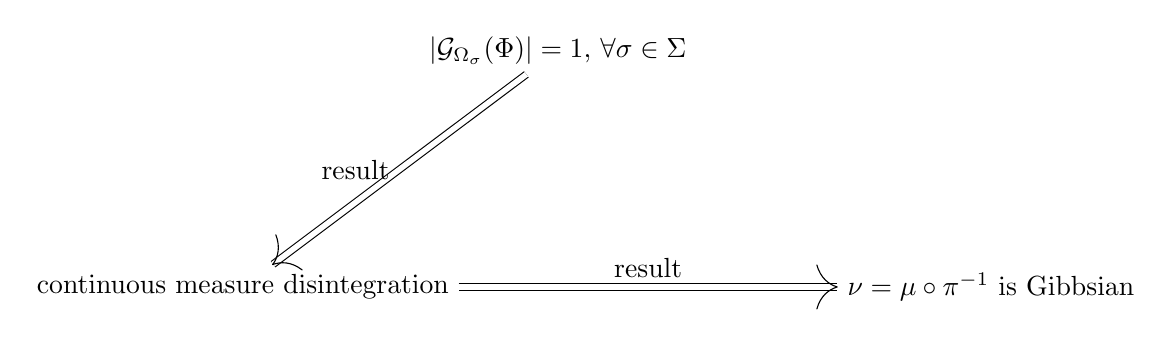
\begin{tikzpicture}
    % Nodes
    \node (A) at (0,0) {continuous measure disintegration};
    \node (B) at (9.5,0) {$\nu=\mu\circ\pi^{-1}$ is Gibbsian};
    \node (C) at (4,3) {$|\G_{\Omega_\sigma}(\Phi)|=1$, $\forall\sigma\in\Sigma$};
    % Double Arrows
    \draw[->, double distance=2pt] (A) -- (B) node[midway, above] {result};
    \draw[->, double distance=2pt] (C) -- (A) node[midway, left] {result};
\end{tikzpicture}\fi

The first example, explored in Chapter \ref{ch:3} is concerned with the fuzzy Potts model, for which a certain sufficient condition was found by H\"aggstr\"om in \cite{Hag}. The alternative proof we give is completely independent, as the original proof in the paper is based on the characterisation of Gibbsianity presented in Proposition \ref{DLR:equiv}, i.e., on verifying the quasilocality. \\

The second example, treated in Chapter \ref{ch:4} is concerned with the random spin-flip dynamics model, explored in \cite{EFHR}. While the paper is not at all concerned with fuzzy Gibbs formalism -- and neither can the general model presented be seen as a fuzzy Gibbs model -- we demonstrate that a special case of the model, for which in particular some interesting results were give, can indeed be easily seen as a fuzzy Gibbs model. Morevoer, we demonstrate that the proof given in the paper are based on a very similar idea, allowing to give a proof using Corollary \ref{Berghout} only by introducing minor modification to the original proof.

% #################################################################################################

\pagebreak

% #################################################################################################
% #################################################################################################
% #################################################################################################

\section{Gibbsianity of fuzzy Potts model}\label{ch:3}

This chapter aims to introduce the fuzzy Potts model and provide an alternative, independent proof of H\"aggstr\"om's result \cite{Hag} about conditions for the Gibbsianity of the involed fuzzy Gibbs measure, using the results due to Berghout and Verbitskiy \cite{Ber}. Moreover, it introduces the notion of random-cluster representations, a powerful tool in the theory of Potts model, which is used in the proof.

% #################################################################################################

\subsection{Classical Potts model}

In this introductory section of the chapter, we define the classical Potts model, with respect to which the fuzzy Potts model will be later defined. We also state the celebrated result the existence of phase transition with respect to the inverse temperature parameter. \\

If what follows, we write $\E^d$ for the edge set associated with the square lattice $\Z^d$ and given $\Lambda\Subset\Z^d$, $\E_\Lambda$ for $\{\sp{x,y}\in\E^d:x,y\in\Lambda\}$ and $\partial\E_\Lambda$ for its ``boundary'', $\{\sp{x,y}\in\E^d:x\in\Lambda,y\notin\Lambda\}$. \\

The Potts model is a natural generalization of (ferromagnetic) Ising model with zero external field ($h=0$), where instead of two possible values ($+1$ and $-1$, as in the context of the Ising model), the spins may assume $q\geq 2$ different values, taking $\A=\set{1,\ldots,q}$ to be the single-spin space, and consequently $\Omega=\set{1,\ldots,q}^{\Z^d}$ to be the configuration space. As in the case of the Ising model, Potts model is a nearest-neighbour model, so the interaction $\Phi$ is defined for $\Lambda=\set{x,y}$, with $x\sim y$ (i.e., $|x-y|=1$) and is given by
$$\Phi_{x\sim y}(\omega) ~=~ 2\1_{\set{\omega(x)\neq \omega(y)}}-1 ~=~ \begin{cases}
1: ~&\omega(x)\neq\omega(y), \\
-1: ~&\omega(x)=\omega(y).
\end{cases}$$
This is indeed analogue to the Ising model the Ising model: clearly, taking $q=2$ and identifying $\set{0,1}$ with $\set{-1,+1}$, one obtains the zero external field Ising model. The above interaction yields the following finite volume Hamiltonian expression: given a finite volume $\Lambda\Subset\Z^d$ we have
$$\H_{\Lambda;\beta}(\omega) ~=~ \beta\sum_{\sp{x,y}\in\E_\Lambda\cup\partial\E_\Lambda}(2\1_{\set{\omega(x)\neq\omega(y)}}-1), \quad \omega\in\Omega.$$
We might, however, take a simpler equivalent interaction, which we justify shortly, in a remark. In the spirit of thermodynamical formalism, the system of Hamiltonians $(\H_\Lambda)_{\Lambda\Subset\Z^d}$ admits a specification $\gamma=(\gamma_\Lambda)_{\Lambda\Subset\Z^d}$, where for each $\Lambda\Subset\Z^d$ we have
\begin{align*}
\gamma_\Lambda:\F_\Lambda\times\Omega_{\Lambda^\c}&\ra (0,1) \\
(\set{\omega_{\Lambda}},\xi_{\Lambda^\c})&\mapsto\gamma_{\Lambda}(\omega_{\Lambda}|\xi_{\Lambda^\c})=\frac{1}{\ZZ_{\Lambda;\beta,q}^\xi}\exp\!\oklepaj{-\H_{\Lambda;\beta}(\omega_\Lambda\xi_{\Lambda^\c})},
\end{align*}
where $\ZZ_{\Lambda;\beta,q}^\xi=\sum_{\tilde{\omega}_\Lambda\in\Omega_\Lambda}\exp\!\oklepaj{-\H_\Lambda(\tilde{\omega}_{\Lambda}\xi_{\Lambda^\c})}$.

\begin{rem}\label{HamiltEquiv}
\begin{itemize}
	\item[(1)] Notice that $$\H_{\Lambda;\beta}(\omega) ~=~ 2\beta\sum_{\sp{x,y}\in\E_\Lambda\cup\partial\E_\Lambda}\1_{\set{\omega(x)\neq\omega(y)}} -\beta(|\E_\Lambda\cup\partial\E_\Lambda|),$$
	where $\beta(|\E_\Lambda\cup\partial\E_\Lambda|)=:C_{\beta,\Lambda}$ is a constant independent of $\omega$, giving us that
	\begin{align*}
	\gamma_{\Lambda}(\omega_{\Lambda}|\omega_{\Lambda^\c}) ~&=~ \frac{\exp(-\H_{\Lambda;\beta}(\omega))}{\sum_{\tilde{\omega}_{\Lambda}\in\Omega_{\Lambda}}\exp(-\H_{\Lambda;\beta}(\tilde{\omega}_{\Lambda}\omega_{\Lambda^\c}))} \\
	&=~ \frac{\exp\!\oklepaj{-2\beta\!\oglati{\sum_{\sp{x,y}\in\E_\Lambda\cup\partial\E_\Lambda}\!\1_{\set{\omega(x)\neq\omega(y)}}}}\!\exp(C_{\beta,\Lambda})}{\exp(C_{\beta,\Lambda})\sum_{\tilde{\omega}_{\Lambda}\in\Omega_{\Lambda}}\exp\!\oklepaj{-2\beta\!\oglati{\sum_{\sp{x,y}\in\E_\Lambda}\!\1_{\set{\tilde{\omega}(x)\neq\tilde{\omega}(y)}} + \sum_{\sp{x,y}\in\partial\E_\Lambda}\!\1_{\set{\tilde{\omega}(x)\neq\omega(y)}}}}} \\
	&=~ \frac{\exp\!\oklepaj{-2\beta\!\oglati{\sum_{\sp{x,y}\in\E_\Lambda\cup\partial\E_\Lambda}\!\1_{\set{\omega(x)\neq\omega(y)}}}}}{\sum_{\tilde{\omega}_{\Lambda}\in\Omega_{\Lambda}}\exp\!\oklepaj{-2\beta\!\oglati{\sum_{\sp{x,y}\in\E_{\Lambda}}\!\1_{\set{\tilde{\omega}(x)\neq\tilde{\omega}(y)}} + \sum_{\sp{x,y}\in\partial\E_{\Lambda}}\!\1_{\set{\tilde{\omega}(x)\neq\omega(y)}}}}},
	\end{align*}
	so the same specification would be obtained by selecting an alternative interaction and system of Hamiltonians
	\begin{align*}
	\Phi_{x\sim y}' ~&=~ 2\1_{\set{\omega(x)\neq\omega(y)}}, \\
	\H_{\Lambda;\beta}'(\omega) ~&=~ 2\beta\sum_{\sp{x,y}\in\E_{\Lambda}\cup\partial\E_\Lambda}\1_{\set{\omega(x)\neq\omega(y)}}.
	\end{align*}
	For the sake of simplicity, from now on, we use will use $\Phi'$ and $(\H_{\Lambda;\beta}')_{\Lambda\Subset\Z^d}$ in our computations instead, and simply denote them by $\Phi$ and $(\H_{\Lambda;\beta})_{\Lambda\Subset\Z^d}$.
	\item[(2)] The interaction we initially used, is often also written in the literature as 
	$$\Phi_{x\sim y}(\omega) ~=~ 1-2\1_{\set{\omega(x)=\omega(y)}}.$$
	Had we used this version, we would in point (1) obtain $\Phi_{x\sim y}'(\omega)=-2\1_{\set{\omega(x)=\omega(y)}}$ instead.
	\item[(3)] There are several other interactions that equivalently define the Potts model, such as $\Phi_{x\sim y}''(\omega)=\1_{\set{\omega(x)\neq\omega(y)}}$ and $\Phi_{x\sim y}'''(\omega)=-\1_{\set{\omega(x)=\omega(y)}}$ for example.
\end{itemize}
\end{rem}

In the spirit of thermodynamical formalism, the (infinite volume) Gibbs measure for $q$-state Potts model on $\Omega$ with inverse temperature $\beta$ is any probability measure on $\Omega$, whose finite-volume conditional probabilities agree with the specification $\gamma$, that is, a measure $\mu\in\M_1(\Omega)$ such that for each $\Lambda\Subset\Z^d$ and $\omega\in\Omega$, one has
$$\mu(\omega~\text{on}~\Lambda|\xi~\text{off}~\Lambda) ~=~ \gamma_\Lambda(\omega_\Lambda|\xi_{\Lambda^\c}),$$
for $\mu$-a.e.~$\xi\in\Omega$.

\begin{rem}
Notice that for any fixed boundary condition $\xi\in\Omega$, the map $\gamma_\Lambda(\pika|\xi_{\Lambda^\c})$ is a probability measure on $\Omega_\Lambda$, which we can denote as $\tilde{\mu}_{\Lambda;\beta,q}^\xi$. We can, in this case, restate $\mu\in\M_1(\Omega)$ to be Gibbs measure for $q$-state Potts model with inverse temperature $\beta$ if for each $\Lambda\Subset\Z^d$ and $\mu$-a.e.~$\xi\in\Omega$, 
$$\mu(\pika~\text{on}~\Lambda|\xi~\text{off}~\Lambda) ~=~ \tilde{\mu}_{\Lambda;\beta,q}^\xi.$$
Moreover, in the spirit of Remark \ref{rem:InfVol}, we can for each $\tilde{\mu}_{\Lambda;\beta,q}^\xi$ define an analogue probability measure on $\Omega$, given by
$$\mu_{\Lambda;\beta,q}^\xi(\omega) ~=~ \1_{\set{\omega_{\Lambda^\c}=\xi_{\Lambda^\c}}}\tilde{\mu}_{\Lambda;\beta,q}^\xi(\omega_\Lambda), \quad \omega\in\Omega,$$
which one uses to obtain thermodynamical limits.
\end{rem}

The Potts model enjoys a similar phase transition result as the Ising model,  stated in the following theorem.

\begin{thm}[\cite{ACCN}, reformulated as in \cite{GHM}]
For $q$-state Potts model on $\Z^d$ with $d\geq 2$, there exists a critical inverse temprature $\beta_c=\beta_c(d,q)\in(0,\infty)$ such that
\begin{itemize}
	\item[(i)] for each $\beta<\beta_c$ there is a unique Gibbs measure, and 
	\item[(ii)] for each $\beta>\beta_c$, there exist $q$ mutually singular Gibbs measures. 
\end{itemize}
\end{thm}

It is worth mentioning that the mutually singular Gibbs measures in the $\beta>\beta_c$ regime are precisely the measures $\mu_{\beta,q}^1,\ldots,\mu_{\beta,q}^q$, where for $i\in\set{1,\ldots,q}$, $\mu_{\beta,q}^i$ is the thermodynamical limit
$$\mu_{\beta,q}^i ~=~ \text{w-}\!\!\lim_{\Lambda\Uparrow\Z^d}\mu_{\Lambda;\beta,q}^{\mathsf{i}},$$
where $\mathsf{i}=\set{i}^{\Z^d}$ is the constant boundary condition. In other words, $\mathrm{extr}(\G_{\Omega}(\Phi_{\beta,q}))=\{\mu_{\beta,q}^1,\ldots,\mu_{\beta,q}^q\}$.

% #################################################################################################

\subsection{Fuzzy Potts model}

We now turn our attention to the fuzzy Potts model, which we define and state the celebrated result about its (non-)Gibbsianity, due to H\"aggstr\"om \cite{Hag}. Moreover, we explain the strategy and structure of our alternative proof of (part of) the said result. \\

Consider the Potts model with spin space $\A=\set{1,\ldots,q}$, $q\geq 2$, on lattice $\L$, say $\L=\Z^d$, which defines a model on $\Omega=\set{1,\ldots,q}^\L$. The \textit{fuzzy Potts model} is defined by considering some integer $1<s<q$, so that the spin space is $\B=\set{1,\ldots,s}$ and the whole model defined on $\Sigma=\set{1,\ldots,s}^\L$. Moreover, we consider a vector $\r=(r_1,\ldots,r_s)\in\N^s$, such that $r_1+\ldots+r_s=q$ and define a fuzzy transformation $\pi_\r:\set{1,\ldots,q}\ra\set{1,\ldots,s}$ by putting 
$$\pi_\r(a) ~:=~ \begin{cases}
1: ~&1\leq a\leq r_1,\\
2: ~&r_1+1\leq a\leq r_1+r_2 \\
\cdots \\
n: ~&\sum_{i=1}^{n-1} r_i + 1\leq a\leq \sum_{i=1}^n r_i,\\
\cdots \\
s: ~&\sum_{i=1}^{s-1}r_i + 1\leq a\leq q=\sum_{i=1}^s r_i,
\end{cases}$$
i.e., $\pi_a=n$ iff $a\in(\sum_{i=1}^{n-1}r_i,\sum_{i=1}^n r_i]\cap \N$, $n\in\set{1,\ldots,s}$. In other words, the entire fuzzy map $\pi=\pi_\r$ is encoded by a single $s$-vector $\r$. While this construction might seem less general than considering an arbitrary fuzzy map $\pi:\A\ra\B$, there is in fact no loss of generally, as one can just reorder the elements in $\A$. \\

Fixing $q\geq 2$, $\beta\geq 0$ and writing $\mu_{\beta,q}^{\Z^d,\xi}$ for the Gibbs measure of the Potts model on $\set{1,\ldots,q}^{\Z^d}$ for boundary condition $\xi$ with inverse temperature $\beta$, the fuzzy transformation $\pi_\r$ induces the fuzzy Gibbs measure 
$$\nu_{\beta,q,\r}^{\Z^d,\xi} ~:=~ \mu_{\beta,q}^{\Z^d,\xi}\circ\pi_\r^{-1}.$$
Of great interest is the potential Gibbsianity of such measure. This was partly answered by H\"aggstr\"om in \cite{Hag}, though -- as we will see -- there remains a gap in the result. Recall that for $q\geq 2$ and $d\geq 2$, there exists $\beta_c(d,q)\in(0,\infty)$ such that for each $\beta<\beta_c(d,q)$, $\mu_{\beta,q}^{\Z^d,0}=\mu_{\beta,q}^{\Z^d,1}=\ldots=\mu_{\beta,q}^{\Z^d,q}$,\footnote{Here, $\mu_{\beta,q}^{\Z^d,0}$ denotes the Gibbs measure corresponding to the free boundary condition.} i.e., there is a unique Gibbs measure of the Potts model on $\set{1,\ldots,q}^{\Z^d}$ with inverse temperature $\beta$, while for each $\beta>\beta_c(d,q)$ there are $q$ mutually singular Gibbs measures, which are precisely $\mu_{\beta,q}^{\Z^d,1},\ldots,\mu_{\beta,q}^{\Z^d,q}$.

\begin{thm}[H\"aggstr\"om, 2003, \cite{Hag}]\label{Haggstrom}
Let $d\geq 2$, $q\geq 3$, $i\in\set{0,1,\ldots,q}$ and $\r=(r_1,\ldots,r_s)$ with $1<s<q$, $r_1+\ldots+r_s=q$, and write $r^*=\min(\set{r_1,\ldots,r_s}\cap\N_{\geq 2})$. Consider a fuzzy Gibbs measure $\nu_{q,\beta,\r}^{\Z^d,i}=\mu_{q,\beta}^{\Z^d,i}\circ\pi_{\r}^{-1}$.
\begin{itemize}
	\item[(i)] For each $\beta<\beta_c(d,r^*)$, the measure $\nu_{\beta,q,\r}^{\Z^d,i}$ is a Gibbs measure.
	\item[(ii)] For any $\beta>\frac{1}{2}\log\frac{1+(r^*-1)p_c(d)}{1-p_c(d)}$, $\nu_{\beta,q,\r}^{\Z^d,i}$ is not a Gibbs measure. Here $p_c(d)$ denotes the critical probability for Bernoulli percolation, see Appendix \ref{app:3}.
\end{itemize}
\end{thm}

\begin{rem}
Given $q',q''\geq 2$ such that $q'\leq q''$, one has $\beta_c(d,q')\leq\beta_c(d,q'')$. The requiring that $\beta$ be smaller than the critical inverse temperature corresponding to the minimal $r_i$ (strictly larger than 1) guarantees that $\beta<\beta_c(d,r_i)$ for all $i=1,\ldots,s$. This indeed yields uniqueness of Gibbs measure for Potts model on $\set{1,\ldots,s_i}^{\Z^d}$ (with this choice of $\beta$) for all $i=1,\ldots,s$. Requirement that $r^*\geq 2$ guarantees that $\beta_c(d,r^*)\in(0,\infty)$.
\end{rem}

In light of the theory from the previous chapter, we are particularly interested in part (i) of the theorem, the Gibbs regime. The van Enter-Fern\'andez-Sokal hypothesis, would suggest that, since for $\beta<\beta_c(d,r^*)$ the Gibbs property is preserved, each $\mu_{\beta,q}^{\Z^d,\xi}$ should admit a continuous disintegration in terms of $\nu_{\beta,q,\r}^{\Z^d,\xi}$. Moreover, proving the latter would -- applying the result of Theorem \ref{thm:DisinImpliesGibbs} -- constitute an alternative and independent proof of Theorem \ref{Haggstrom}.(i). \\

Given Theorem \ref{thm:TjurFibre}.(ii), it is sufficient to verify (for a fixed $\beta<\beta_c(d,r^*))$, that for each $\sigma\in\Sigma=\set{1,\ldots,s}^{\Z^d}$, there is a unique Gibbs measure for $q$-Potts model with inverse temperature beta on the fibre $\Omega_\sigma=\pi_\r^{-1}(\sigma)$, i.e., that
$$|\G_{\Omega_\sigma}(\Phi_{\beta,q})| ~=~ 1, \quad \forall \sigma\in\Sigma.$$
Luckily, one can express the fibres in a rather nice way, allowing for an easier procedure. Given $\sigma\in\Sigma$, we simply have (with tiny but non-ambiguous abuse of notation)
$$\Omega_\sigma ~=~ \pi_{\r}^{-1}(\sigma) ~=~ \prod_{x\in\Z^d}\pi_{\r}^{-1}(\sigma(x)).$$
Writing $\A_j:=\pi_{\r}^{-1}(j)$ and $U_j:=\set{x\in\Z^d:\pi_{\r}(\sigma(x))=j}$, $j=1,\ldots,s$, we could also write
$$\Omega_\sigma ~=~ \bigotimes_{j=1}^s\A_j^{U_j} ~:=~ \prod_{i\in\Z^d}\begin{cases}\A_1:~&i\in U_1,\\
\cdots\\
\A_s:~&i\in U_s.\end{cases}$$
One way of proving the uniqueness of $q$-Potts Gibbs measure on such $\Omega_\sigma$ for appropriate inverse temperature $\beta<\beta_c(d,r^*)$ is via the following two steps (so far stated informally):
\begin{itemize}
	\item[(1)] Given the assumption on $\beta$, we know that for each $j=1,\ldots,s$, there is a unique Gibbs measure for Potts model on $\A_j^{\Z^d}$ with inverse temperature $\beta$. We wish to show that this implies also uniqueness of Gibbs measure for Potts model on $\A_j^{U_j}$, given the same inverse temperature.
	\item[(2)] Given the uniqueness of Gibbs measure for Potts model on $\A_j^{U_j}$ with inverse temperature $\beta$ for all $j=1,\ldots,s$, we need to show that this implies the uniqueness of Gibbs measure for Potts model on $\bigotimes_{j=1}^s \A_j^{U_j}$, given the same inverse temperature.
\end{itemize}
It is clear that it is enough to verify the above steps for $s=2$, as the argument for larger $s$ follows immediately by induction. To be precise about what we wish to prove, we formulate two propositions that are to be verified, in order to obtain the conclusion.

\begin{prop}[Part 1]\label{FP:part1}
Let $\beta<\beta_c(d,q)$ (i.e., there's unique Gibbs measure for Potts model on $\set{1,\ldots,q}^{\Z^d}$) and let $U\subset\Z^d$. Then, there's a unique Gibbs measure for Potts model on $\set{1,\ldots,q}^U$ with inverse temprature $\beta$.\footnote{The subset $U$ is understood to be equipped with an edge set $\E_U=\set{\sp{x,y}:x\sim y,\,x,y\in U}$}
\end{prop}

\begin{prop}[Part 2]\label{FP:part2}
Suppose $U,V\subset\Z^d$ form a partition of $\Z^d$ and let $\AA,\AB$ be disjoint alphabets. Suppose that for $\beta\in(0,\infty)$, Potts model with inverse temperature $\beta$ admits a unique Gibbs measure on both $\AA^U$ and $\AB^V$ (i.e., $|\G_{\AA^U}(\Phi_{\beta,|\AA|}|=|\G_{\AB^V}(\Phi_{\beta,|\AB|})|=1$). Then the same is the case for the Potts model with inverse temperature $\beta$ on $\AA^U\otimes\AB^V$, i.e.,
$$|\G_{\AA^U\otimes\AB^V}(\Phi_{\beta,|\AA|+|\AB|})| ~=~ 1.$$
\end{prop}

\subsection{Outline of H\"aggstr\"om's proof}\label{ProofComparison}

In light of the fact that our proof of absence of phase transition in the $\beta<\beta_c(d,r^*)$ regime constitutes an alternative proof of Theorem \ref{Haggstrom}.(i), it is worth outlining the proof given in \cite{Hag}, to highlight the differences between the two methods and to hopefully convince the reader of the significance of our alternative proof as well as of the possible applications of Corollary \ref{Berghout} in general. \\

H\"aggstr\"om's proof first and foremost relies on the alternative formulation of Gibbs measures via quasilocality and uniform non-nullness, as well as the fact that fuzzy Gibbs measures are always uniformly non-null, hence non-Gibbsianity is always the result of non-quasilocality. It is thus sufficient to verify, that for any choice of $\Delta\Subset\Z^d$, $\sigma\in\{1,\ldots,s\}^{\Z^d}$, $i\in\{0,1,\ldots,q\}$ and $\varepsilon>0$, there exists $N\in\N$ such that for any $n\geq N$ and any choice of $\eta,\eta'\in\set{1,\ldots,s}^{\Z^d}$ that agree on $\Lambda_n\setminus\Delta$,
$$|\nu_{\beta,q,\r}^{\Z^d,i}(\sigma_{\Delta}|\eta_{\Delta^\c})-\nu_{\beta,q,\r}^{\Z^d,i}(\sigma_\Delta|\eta_{\Delta^c}')| ~\leq~ \varepsilon;$$
here $(\Lambda_n)_{n\in\N}$ is the underlying increasing sequence of finite volumes. \\

The author first remarks that it is sufficient to show, that given random fuzzy Potts configurations $Y$ and $Y'$, such that $Y\sim\nu_{\beta,q,\r}^{\Z^d,i}(\pika|\eta_{\Delta^\c})$ and $Y'\sim\nu_{\beta,q,\r}^{\Z^d,i}(\pika|\eta_{\Delta^\c})$, one can construct a coupling (see Appendix \ref{app:2}) $\Q$ of $Y,Y'$, such that
$$\Q(Y_{\Delta}=Y_{\Delta}') ~\geq~ 1-\varepsilon.$$
This can indeed be guaranteed by showing that with a probability at least $1-\varepsilon$, there exists a (random) edge set $E\subseteq\E_{\Lambda_n\setminus\Delta}=\set{\sp{x,y}:x,y\in\Lambda_n\setminus\Delta}$, which separates $\Delta$ from $\Lambda_n^\c$ -- in a sense that any path from $\Delta$ to $\Lambda_n^\c$ must pass through at least on edge from $E$ -- and is such that given certain random configurations $U,U'$ corresponding to $Y,Y'$ (in the sense of the random-cluster model, see Section \ref{sec:RandomCluster}), $U_E=U_E'\equiv 0$. \\

In light of Definition \ref{def:EdwardsSokal}, H\"aggstr\"om first considers the (joint) distribution $\PP$ of $(\tilde{U},\tilde{X},\tilde{Y})$, where $\tilde{U}$ is a random edge configuration, distributed according to the random-cluster measure $\phi_{p,q}^{\Z^d,1}$ (see Section \ref{subsec:RCinf}), $\tilde{X}$ is a corresponding configuration in $\set{1,\ldots,q}^{\Z^d}$ obtained by assigning each connected component of $(\Z^d,U)$ a $\mathrm{Unif}(1,\ldots,q)$-drawn sign (which results in $\tilde{X}$ having a marginal distribution $\mu_{\beta,q}^{\Z^d, i}$, see Cor.~\ref{cor:EdwardsSokal}.(i)) and $Y=\pi_\r(X)$ (which results in $\tilde{Y}$ having a marginal distribution $\nu_{\beta,q,\r}^{\Z^d,i}$). Given $\Delta$ as above and $\eta,\eta'$ agreeing on $\Lambda_n\setminus\Delta$ (as above) one can define a coupling $\Q$ of 
$$(U,X,Y)\sim\PP(\pika|Y_{\Delta^c}=\eta_{\Delta^c}),~(U',X',Y')\sim\PP(\pika|Y_{\Delta^c}'=\eta_{\Delta^\c}')~\text{and}~U''\sim\phi_{p,r_*}^{\Z^d,1};$$
this will be the coupling for which it is argued that $\Q(Y_{\Delta}=Y_{\Delta}')\geq 1-\varepsilon$. \\

An appropriate $N$ is selected rather intuitively: the event that an infinite cluster exists has $\phi_{p,r^*}^{\Z^d,1}$-probability zero for any $\beta<\beta_c(d,r^*)$ (see Theorem \ref{ACCN}), from which it follows that
$$\phi_{p,r^*}^{\Z^d,1}(\Delta\leftrightarrow\Lambda_n^\c) ~\xrightarrow{n\ra\infty}~ 0,$$
so we let $N$ be the first integer for which the probability on the left-hand side is at most $\varepsilon$. \\

It is established through various technical lemmas, that $\Q$ can be constructed so that there exists a finite subgraph $\tilde{G}=(\tilde{V},\tilde{E})$ that is isolated from the rest of the lattice by $U$- and $U'$-closed edges -- which allows us to assume $(U_{\tilde{E}},X_{\tilde{V}},Y_{\tilde{V}})=(U_{\tilde{E}}',X_{\tilde{V}}',Y_{\tilde{V}}')$ in the coupling -- and is such that $\tilde{V}$ contains $\Delta$ with $\Q$-probability at least $1-\varepsilon$.\footnote{The latter has everything to do with our choice of $N$ above and the fact that $\Delta\not\subseteq\tilde{V}$ implies existence of a path from $\Delta$ to $\Lambda_n^\c$.} Since $\Delta\subseteq\tilde{V}$ along with $Y_{\tilde{V}}=Y_{\tilde{V}}'$ implies that $Y_{\Delta}=Y_{\Delta}'$, one can infer that 
$$\Q(Y_{\Delta}=Y_{\Delta}') ~\geq~ \Q(\Delta\subseteq\tilde{V}) ~\geq~ 1-\varepsilon,$$
which gives the conclusion.\footnote{This exact line of argumentation requires an additional assumption that $r_j\geq 2$ for each $j=1,\ldots,s$. However, only a simple modification is needed to obtain the proof for general $\r$.} \\

In contrast, being equipped with Corollary \ref{Berghout} allows us to fix $Y$ and prove the fact by studying the distribution of $X^{(Y)}=\pi_\r^{-1}(Y)$. In particular, we have to show that for any realization of $Y$, there's a unique Gibbs-Potts measure that can be seen as the law of $X^{(Y)}$. This is done -- as explained before -- by first showing that the preimage of each monochromatic component of $Y$ admits a unique Gibbs-Potts measure (which ends up being purely an exercise about random-cluster measures) and secondly that their product (measure) is a unique Gibbs-Potts measure on $\pi_\r^{-1}(Y)$. Overall, such proof -- while not necessarily shorter -- is subject to less technical nuance.

% #################################################################################################

\subsection{Preliminaries, part 1: stochastic domination}

In this and the next section, we will introduce some tools, which will be used to prove Proposition \ref{FP:part1}. This section will cover the basics on stochastic domination, a well-established tool in mathematical statistical mechanics. In the section that follows, we introduce the theory of random-cluster representations, which are important in study of the Potts model in particular. \\

Assume firstly that $\A\subset\R$ is linearly ordered; in our case, we are generally assuming $\A$ to be finite, though this theory can be extended to closed subsets of $\R$. Then linear order of $\A$ induces a natural (coordinatewise) partial order on $\Omega=\A^\L$: given two configurations $\xi,\xi'\in\Omega$, we write
$$\xi\preceq\xi' ~\iff~ \xi(i)\leq\xi'(i),~\forall i\in\L.$$
This allows us to introduce a notion of increasing functions:

\begin{df}[Increasing functions and events]
~
\begin{itemize}
	\item[(1)] We say that a function $f:\Omega\ra\R$ is \textit{increasing} (or \textit{non-decreasing}), if for each $\xi,\xi'\in\Omega$, $\xi\preceq\xi'$ implies $f(\xi)\leq f(\xi')$. 
	\item[(2)] Equipped with the previous notion, we say that an event $A$ (or a simply $A\subset\Omega$ measurable) is \textit{increasing} if $\1_A$ is an increasing function.
\end{itemize}
\end{df}

\begin{ex}
A very simple example of an increasing event is $\set{x\leftrightarrow\infty}$, the event that $x\in\L$ belongs to an infinite cluster, see Appendix \ref{app:3}. Indeed, if $x$ belongs to some infinite cluster $C$, and we obtain a cluster $C'$ by opening some additional edges of the percolation configuration, we get that $C\subseteq C'$ and hence $x\in C'$. The same holds for the events of type $\set{\Lambda\leftrightarrow\Delta}$ where $\Lambda,\Delta$ are disjoint.
\end{ex}

 This allows us to define a certain partial order on $\M_1(\Omega)$, the set of probability measures on $\Omega$, which turns out to come very handy in the statistical mechanics of lattice systems. In particular, we will heavily rely on this notion in our proof of Proposition \ref{FP:part1}.
 
\begin{df}[Stochastic domination]
Let $\mu$ and $\mu'$ be probability measures on $\Omega$. We say that $\mu$ is \textit{stochastically dominated} by $\mu'$, writing $\mu\preceq_\D\mu'$, if
$$\int f\,\d\mu ~\leq~ \int f\,\d\mu'$$
for each increasing $f\in\BM(\Omega)$.
\end{df}

\begin{rem}
An important fact to note is, that given $\mu\preceq_\D\mu'$ and an increasing event $A$ (such as $\set{x\leftrightarrow\infty}$ for example), one has 
$$\mu(A) ~\leq~ \mu'(A).$$
Note that there exists an analogue notion of \textit{decreasing events}, for which a reverse inequality would hold.
\end{rem}

While the notions presented above are sufficient for us to carry out the proof, we shall present two fundamental results, which indeed hide in the proof of the known results we will use in our proof. First is the Holley's Theorem, which is a powerful way of verifying stochastic domination between concrete measures:
\begin{thm}[Holley, Theorem 4.8 in \cite{GHM}]\label{Holley}
Let $\A\subset\R$ finite as before and suppose $\L$ is finite as well. We now consider $\mu,\mu'\in\M_1(\Omega)$ and assume that $\mu'$ is irreducible\footnote{This means that any two configurations in $\supp(\mu)$ can be reached from one another via successive coordinate changes without ``passing through'' $\supp(\mu)^\c$.} and that it assigns a positive probability to $\preceq$-maximal element of $\Omega$. Suppose that
$$\mu(\omega(x)\geq a|\xi~\text{off}~x) ~\leq~ \mu'(\omega(x)\geq a|\eta~\text{off}~x), \quad \omega\in\Omega,$$
for any choice of $x\in\L$, $a\in \A$, and $\xi,\eta\in\Omega_{\L\setminus\set{x}}$ with $\xi\preceq\eta$ and $\mu(\xi~\text{off}~x),\mu'(\eta~\text{off}~x)>0$. Then $\mu\preceq_\D\mu'$.
\end{thm}

This result is in particularly useful in the case of percolation measures (i.e., measures on $\set{0,1}^E$, with $E$ some edge set), since due to $\A=\set{0,1}$, one only need to check the inequality for $a=1$ (one for $a=0$ being fulfilled automatically). \\

The next import result is the Strassen's Theorem, which sheds light on an important connection between stochastic domination and the coupling theory (Appendix \ref{app:2}). 

\begin{thm}[Strassen, Theorem 4.6 in \cite{GHM}]
Let $\mu,\mu'\in\M_1(\Omega)$. The following are equivalent:
\begin{itemize}
	\item[(i)] $\mu\preceq_\D\mu'$
	\item[(ii)] For any choice of increasing bounded continuous function $f:\Omega\ra\R$, $\int f\,\d\mu\leq \int f\,\d\mu'$.
	\item[(iii)] There exists a coupling $\PP$ of $X\sim\mu$ and $X'\sim\mu'$, such that $\PP(X\preceq X')=1$.
\end{itemize}
\end{thm}

While one is usually mostly interested in the equivalence (i)$\Leftrightarrow$(iii), the equivalence (i)$\Leftrightarrow$(ii) also gives an interesting immediate corollary, which is that stochastic domination is preserved under weak limits.

% #################################################################################################

\subsection{Preliminaries, part 2: random-cluster representations}\label{sec:RandomCluster}

We now present the \textit{random-cluster representations}, first introduced by Fortuin and Kesteleyn in \cite{FK},\cite{For1},\cite{For2} (after whom it is also known as the \textit{Fortuin-Kesteleyn model}, or simply \textit{FK model}), which is an indispensable tool for studying phase transition in Ising and Potts model. First, we will introduce the theory for the case of finite graphs, which will give the much needed intuition, and continue to extend it to the more useful infinite lattice setting. The section is almost entirely based on \cite{GHM} and \cite{Gri}.

% *************************************************************************************************

\subsubsection{random-cluster on a finite graph}

Throughout the section, we consider a finite graph $G=(V,E)$. The \textit{random-cluster measure}, defined shortly, is a percolation measure, i.e., a probability measure defined on $\set{0,1}^E$. Given $\eta\in\set{0,1}^E$, we write $G_\eta=(V,\eta)$ for the subgraph of $G$ given by 
$$G_\eta ~=~ \set{V,\set{e\in E:\eta(e)=1}}.$$
Moreover, we define the quantity $k(\eta)$, which represents the number of connected components in $G_\eta$ (including the isolated vertices). 

\begin{df}
The \textit{random-cluster measure} $\phi_{p,q}^G$ for $G$, with parameters $p\in[0,1]$ and $q>0$, is the probability measure on $\set{0,1}^E$, given by
$$\phi_{p,q}^{G}(\eta) ~=~ \frac{1}{\ZZ_{p,q}^G}\set{\prod_{e\in E}p^{\eta(e)}(1-p)^{1-\eta(e)}}q^{k(\eta)}, \quad \eta\in\set{0,1}^E,$$
where $\ZZ_{p,q}^{G}$ is the normalizing constant.
\end{df} 

Clearly, $q=1$ yields Bernoulli percolation measure, $\phi_{p,1}^G=\psi_{p}^G$, see Appendix \ref{app:3}; this is the only case where $\phi_{p,q}^G$ can be seen as a product measure (outside $p=1$ and $p=0$). \\

It turns out, that for the case of $q\in\set{2,3,\ldots}$, there is an intimate relation with the Potts model. Writing $\H_\beta^G$ for the Hamiltonian of Potts model on $\set{1,\ldots,q}^V$ (in the sense of the finite volume setting, see Section \ref{FiniteVolumeSetting}, we write
$$\mu_{\beta,q}^G(\omega) ~=~ \frac{1}{\ZZ_{\beta,q}^G}\exp(-\H_\beta^G(\omega)), \quad \omega\in\set{1,\ldots,q}^V,$$
for the finite volume Gibbs measure for Potts model on $\set{1,\ldots,q}^V$ with inverse temperature $\beta$. It turns out that $\mu_{\beta,q}^G$ and $\phi_{p,q}^G$ can be very fruitfully related via a certain coupling, introduced by Swendsen and Wang in \cite{SW} and further explored  by Edwards and Sokal in \cite{ES}.

\begin{df}\label{def:EdwardsSokal}
Fix $q\in\set{2,3,\ldots}$ and $p\in[0,1]$. Let now $\PP_{p,q}^G$ be a probability measure on $\set{1,\ldots,q}^V\times\set{0,1}^E$, which corresponds to picking a random element according to the following procedure:
\begin{itemize}
	\item[(1)] To each $x\in V$, assign $X(x)\sim\mathrm{Unif}(1,\ldots,q)$, and to each $e\in E$, $Y(e)\sim\mathrm{Ber}(p)$, independently for all vertices and edges.
	\item[(2)] Condition on the event that for any choice of $x\sim y$, $X(x)\neq X(y)$ imples $Y((x,y))=0$, i.e., vertices assuming different spin values are not connected by open edges.
\end{itemize}
In fact, one has
$$\PP_{p,q}^G(\omega,\eta) ~\propto~ \prod_{e=(x,y)\in E}p^{\eta(e)}(1-p)^{1-\eta(e)}\1_{\set{(\omega(x)-\omega(y))\eta(e)=0}},$$
where the event $\set{(\omega(x)-\omega(y))\eta(e)=0}$ enforces precisely the conditioning described in (2). We call $\PP_{p,q}^G$ the \textit{Edwards-Sokal measure}.
\end{df}

\begin{thm}[\cite{GHM}, Theorem 6.2]
Taking $\beta=\frac{1}{2}\log(1-p)$, $\PP_{p,q}^G$ constitutes a coupling of $\mu_{\beta,q}^G$ and $\phi_{p,q}^G$.	
\end{thm}

The usefulness of this coupling can be seen in the following corollary:

\begin{cor}\label{cor:EdwardsSokal}
One can very simply ``obtain'' $\mu_{\beta,q}^G$ from $\phi_{p,q}^G$, and the other way around.
\begin{itemize}
	\item[(i)] Let $p=1-e^{-2\beta}$. Suppose we pick a $\set{1,\ldots,q}^V$-values random configuration $X$ as follows:
	\begin{itemize}
		\item[(1)] Pick a random edge configuration $Y\sim\phi_{p,q}^G$.
		\item[(2)]  For each connected component $C$ of $G_Y=(V,Y)$, pick $Z_C\sim\mathrm{Unif}(1,\ldots,q)$ (for each $C$ independently) and assign to each vertex in $C$ the value assumed by $Z_C$.
	\end{itemize}
	Then, $X\sim\mu_{\beta,q}^G$.
	\item[(i)] Let again $p=1-e^{-2\beta}$. Suppose now we pick a $\set{0,1}^E$-valued random edge configuration $Y$ according to the following procedure:
	\begin{itemize}
		\item[(1)] Pick a random configuration $X\sim\mu_{\beta,q}^G$.
		\item[(2)] For each $e=\sp{x,y}\in E$ independently, assign
		$$Y(e) ~\sim~ \begin{cases}
		\mathrm{Ber}(p): ~&X(x)=X(y),\\
		\delta_0: ~&X(x)\neq X(y).
		\end{cases}$$
	\end{itemize}
	Then, $Y\sim\phi_{p,q}^G$.
\end{itemize}
\end{cor}

% *************************************************************************************************

\subsubsection{Infinite-volume random-cluster and phase transitions}\label{subsec:RCinf}

We now proceed with introducing the notion of an infinite-volume random-cluster measure. While we will define them for the lattice $(\Z^d,\E^d)$, the construction can be done on a much more general class of infinite graphs $G=(V,E)$. An alternative to $\Z^d$ we will be in particular interested in will be its subgraphs $(U,\E_U)$, $U\subset\Z^d$. \\

Letting $G=(V,E)$ be a locally finite infinite graph, we consider finite simply connected region $F\subset E$ and write $V_F\subset V$ for the set of vertices to which at least one member of $F$ is incident to. Given a boundary condition $\xi\in\set{0,1}^E$, we define a \textit{random-cluster distribution} $\phi_{F;p,q}^{\xi}$, given by 
$$\phi_{F;p,q}^{\xi}(\eta) ~=~ \frac{1}{\ZZ_{F;p,q}^\xi}\1_{\set{\eta_{F^\c}=\xi_{F^\c}}}\!\set{\prod_{e\in F}p^{\eta(e)}(1-p)^{1-\eta(e)}}q^{k(\eta,F)}, \quad \eta\in\set{0,1}^E,$$
where $\ZZ_{F;p,q}^\xi$ is the normalization constant and $k(\eta,F)$ the number of connected components of $\eta$ which intersect $V_F$.

\begin{df}
A probability measure $\phi\in\M_1(\set{0,1}^E)$ is a \textit{random-cluster} measure (with parameters $p\in[0,1]$ and $q>0$) if
$$\phi(\eta_F|\xi_{F^\c}) ~=~ \phi_{F;p,q}^\xi(\eta)$$
for all finite simply connected $F\subset E$, $\phi$-a.a.~$\xi\in\set{0,1}^E$ and all $\eta\in\set{0,1}^E:\eta_{F^\c}=\xi_{F^\c}$.
\end{df}

A very handy property of random-cluster measures, which works great in tandem with Holley's Theorem (which is very easy to see given the remark we gave about how nicely the latter works with percolation measures) is the following:
\begin{prop}[Lemma 6.18 in \cite{GHM}]\label{prop:e open}
A probability measure $\phi\in\M_1(\set{0,1}^E)$ is a random-cluster measure (for $p\in[0,1]$ and $q>0$) if and only if for all $e=\sp{x,y}\in E$ and $\phi$-a.a.~$\xi\in\set{0,1}^E$, one has
$$\phi(e~\text{is open}|\xi_{E\setminus\set{e}}) ~=~ \begin{cases}
p, ~&x\leftrightarrow y~\text{in}~G_\xi=(V,\xi), \\
\frac{p}{p+(1-p)q},~&\text{otherwise}.
\end{cases}$$
\end{prop}

However, we are interested in a very particular class of random-cluster measures, which are rather analogue to the infinite-volume limit Gibbs measures introduced in Chapter \ref{ch:1}. We will now define it for the lattice $(\Z^d,\E^d)$, but it is not difficult to see that the same can be done for $(U,\E_U)$, $U\subset\Z^d$. Letting $\Lambda\Subset\Z^d$, we fix parameters $p\in[0,1]$, $q>0$ and a boundary condition $\xi\in\set{0,1}^{\E^d}$, we define $\phi_{\Lambda;p,q}^{\Z^d,\xi}$ via
$$\phi_{\Lambda;p,q}^{\Z^d,\xi}(\eta) ~=~ \frac{1}{\ZZ_{\Lambda;p,q}^{\Z^d,\xi}}\1_{\set{\eta_{\E_\Lambda^\c}=\xi_{\E_\Lambda^\c}}}\!\set{\prod_{e\in\E_\Lambda}p^{\eta(e)}(1-p)^{1-\eta(e)}}q^{k(\eta,\Lambda)}, \quad \eta\in\set{0,1}^{\E^d},$$
where $\ZZ_{\Lambda;p,q}^{\Z^d,\xi}$ is the normalization constant and $k(\eta,\Lambda)$ the number of connected components of $(\Z^d,\eta)$ that intersect $\Lambda$. The obvious similarities with previously defined $\phi_{F;p,q}^{\xi}$ justify the perhaps uncomfortably similar notation. \\

Notice that the only way the values inside $\E_\Lambda$ are affected by the boundary condition is through $k(\eta,\Lambda)$. Consider the connected components only within $\Lambda$; the way that the boundary condition can affect the counting of $k(\eta,\Lambda)$ is if there exists an $\xi$-open path in $\E_\Lambda^\c$, that connects two different connected components in $\Lambda$ -- they are now no longer counted as two separate connected components, but a single one. That way, for $\xi\equiv 1$, there is a ``single'' connected component touching $\partial\Lambda$, while for $\xi\equiv 0$, the boundary doesn't affect $k(\eta,\Lambda)$. The latter in particular will be important latter. \\

We now proceed to list some important properties of the measures defined above, which will be of major importance to our proof of Proposition \ref{FP:part1}.  \\

The first one show us, how the boundary condition influences the stochastic ordering of the given measures:
\begin{prop}[Lemma 4.14.(b) in \cite{Gri}]\label{RC:boundarydomination}
For $\xi,\zeta\in\set{0,1}^{\E^d}:\xi\preceq\zeta$,
$$\phi_{\Lambda;p,q}^{\Z^d,\xi} ~\preceq_\D~ \phi_{\Lambda;p,q}^{\Z^d,\zeta}.$$
In fact, it is sufficient that $\xi(e)\leq\zeta(e)$ for all $e\in\E_\Lambda^\c$.
\end{prop}

Next, we describe how the stochastic ordering is influenced by the choice of finite volume $\Lambda$, assuming a fixed boundary condition $\xi\equiv 1$, and what this tells us about the infinite-volume (weak) limit:
\begin{prop}[Theorem 4.19.(a) in \cite{Gri}; equation (29) in \cite{GHM}]\label{RC:decr converg}
For $\Lambda\subset\Delta\Subset\Z^d$,
$$\phi_{\Delta;p,q}^{\Z^d,1} ~\preceq_\D~ \phi_{\Lambda;p,q}^{\Z^d,1}.$$
In particular,
$$\phi_{p,q}^{\Z^d,1} ~=~ \text{w-}\!\!\lim_{\Lambda\Uparrow\Z^d}\phi_{\Lambda;p,q}^{\Z^d,1}$$
exists, with $\phi_{\Lambda;p,q}^{\Z^d,1}(A)\downarrow\phi_{p,q}^{\Z^d,1}(A)$ for any increasing event $A$.
\end{prop}
\begin{rem}
We will use this fact not only for $\phi_{\Lambda;p,q}^{\Z^d,1}$ on $(\Z^d,\E^d)$, but also for $\phi_{\Lambda\cap U;p,q}^{U,1}$ on $(U,\E_U)$, $U\subset\Z^d$. It can be easily deducted from the proof in \cite{Gri} that such a generalization does indeed hold.
\end{rem}
The last one is concerned with the consistency of conditional probabilities. It might not appear very relevant at the moment, but will play a huge importance in the proof that follows.
\begin{prop}[Lemma 4.13 in \cite{Gri}]\label{RC:conditionalconsisteny}
Let $\Lambda\subset\Delta\Subset\Z^d$. Then for any choice of $\eta\in\set{0,1}^{\E^d}:\eta_{\E_\Lambda^\c}=\xi_{\E_\Lambda^\c}$,
$$\phi_{\Delta;p,q}^{\Z^d,\xi}(A|\F_\Lambda)(\eta) ~=~ \phi_{\Lambda;p,q}^{\Z^d,\xi}(A), \quad \forall A\in\F.$$
\end{prop}

We conclude this section by finally listing result due to Aizenman, Chayes, Chayes and Newman that reveals how the intimate between random-cluster measures and Gibbs measures of the Potts model can be fruitful in studying the phase transitions in the latter. While it is again stated for the case of $\Z^d$, all the arguments constituting the proof can be -- as stated in the Section 6.3 in \cite{GHM} -- carried out for an arbitrary (locally finite) infinite graph (hence also in those of form $(U,\E_U)$, $U\subset\Z^d$).

\begin{thm}[Aizenman, Chayes, Chayes, Newman, \cite{ACCN}; Theorem 6.10 in \cite{GHM}]\label{ACCN} Let $\beta>0$, $p=1-e^{-2\beta}$, $x\in\Z^d$ and $i\in\set{1,\ldots,q}$. The following are equivalent:
\begin{itemize}
	\item[(i)] $|\G_{\set{1,\ldots,q}^{\Z^d}}(\Phi_{\beta,q})|=1$, i.e., there is a unique Gibbs measure for the $q$-state Potts model on $\Z^d$ with inverse temperature $\beta$,
	\item[(ii)] $\mu_{\beta,q}^{\Z^d,i}(\omega:\omega(x)=i)=\frac{1}{q}$,
	\item[(iii)] $\phi_{p,q}^{\Z^d,1}(x\leftrightarrow\infty)=0$.
\end{itemize}
\end{thm}

% #################################################################################################

\subsection{Proof of Proposition \ref{FP:part1}}

Given the equivalence (i)$\Leftrightarrow$(iii) in Theorem \ref{ACCN}, it is sufficient to prove the following:
\begin{lem}\label{part1:MainLemma}
Let $U\subset\Z^d$ and consider $(U,\E_U)$, which we refer to just by $U$. If for certain $\beta$ (writing $p=1-e^{-2\beta}$) one has $\phi_{p,q}^{\Z^d,1}(x\leftrightarrow\infty)=0$, then also
$$\phi_{p,q}^{U,1}(x\leftrightarrow\infty) ~=~ 0.$$
\end{lem}
\begin{rem}
Note that while we write $\set{x\leftrightarrow\infty}$ in both cases, we are in the first case thinking of the union of configurations in $\set{0,1}^{\E^d}$ and in the second case of ones in $\set{0,1}^{\E_U}$.
\end{rem}

Before we prove Lemma \ref{part1:MainLemma}, we enrich our toolbox a little further, to make our job as easy as possible.

\begin{lem}\label{Part1:Lemma1}
Let $\mu,\nu_1,\ldots,\nu_n$ be such that $\mu\preceq_\D\nu_i$ for all $i=1,\ldots,n$, and let $(p_1,\ldots,p_n)$ be a probability vector. Then
$$\mu ~\preceq_\D~ p_1\nu_1+\ldots+p_n\nu_n.$$
\end{lem}
\begin{proof}
By definition of $\preceq_\D$, $\int f\,\d\mu\leq\int f\,\d\nu_i$ for each increasing $f\in\BM(\Omega)$. It thus follows that
\begin{align*}
\int f\,\d\mu ~&=~ \sum_{i=1}^n p_i\int f\,\d\mu ~\leq~ \sum_{i=1}^n p_i\int f\,\d\nu_i ~=~ \int f\,\d[p_1\nu_1+\ldots p_n\nu_n]
\end{align*}
for any increasing $f\in\BM(\Omega)$ which yields the conclusion.
\end{proof}

\begin{lem}\label{Part1:Lemma2}
Let $\Lambda\subset\Delta$ and let $\xi\in\set{0,1}^{\E^d}$ be such that $\xi(e)=0$ for all $e\in\E_\Delta\setminus\E_\Lambda$. Then
$$\phi_{\Lambda;p,q}^{\Z^d,\xi} ~\preceq_\D~ \phi_{\Delta;p,q}^{\Z^d,\xi}.$$
\end{lem}

\begin{proof}
Consider some $A\subseteq\E_\Delta\setminus\E_U$; since $\xi_{\E_\Delta\setminus\E_\Lambda}\equiv 0$, we have $\xi+\1_A\in\set{0,1}^{\E^d}$ again and it is clear from definition that
$$\phi_{\Delta;p,q}^{\Z^d,\xi} ~=~ \phi_{\Delta;p,q}^{\Z^d,\xi+\1_A}.$$
It thus follows from Proposition \ref{RC:conditionalconsisteny} that for any choice of $\eta\in\set{0,1}^{\E^d}$ that agrees with $\xi+\1_A$ on $\E_\Lambda^\c$,
$$\phi_{\Delta;p,q}^{\Z^d,\xi}(\pika|\F_\Lambda)(\eta) ~=~ \phi_{\Delta;p,q}^{\Z^d,\xi+\1_A}(\pika|\F_\Lambda)(\eta) ~=~ \phi_{\Lambda;p,q}^{\Z^d,\xi+\1_A}.$$ 
Writing $[\xi+\1_A]:=\set{\eta:\eta\equiv \xi+\1_A~\text{off}~\E_\Lambda}\in\F_\Lambda$, we can see that cylinders of this form constitute a finite partition of $\supp(\phi_{\Delta;p,q}^{\Z^d,\xi})$. We write $n$ for its cardinality and $(A_1,\ldots,A_n)$ for (some) enumeration of $\set{A\subseteq\E_\Delta\setminus\E_\Lambda}$. Note also that since $\F_\Lambda$ can be seen as generated by edges of $\E_\Lambda^\c$, one has 
$$\phi_{\Delta;p,q}^{\Z^d,\xi}(\pika|\F_\Lambda)(\eta) ~=~ \phi_{\Delta;p,q}^{\Z^d,\xi}(\pika|[\xi+\1_A]), \quad \eta\in[\xi+\1_A].$$
Writing $p_i$ for the $\phi_{\Lambda;p,q}^{\Z^d,\xi}$-probability of edges in $\E_\Delta\setminus\E_\Lambda$ agreeing with $\1_{A_i}$, the Law of Total Probability yields
\begin{align*}
\phi_{\Delta;p,q}^{\Z^d,\xi} ~&=~ \sum_{i=1}^n p_i\cdot\phi_{\Delta;p,q}^{\Z^d,\xi}(\pika|[\xi+\1_{A_i}]) \\
&=~ \sum_{i=1}^n p_i\cdot\phi_{\Delta;p,q}^{\Z^d,\xi}(\pika|\F_\Lambda)([\xi+\1_{A_i}]) \\
&=~ \sum_{i=1}^n p_i\cdot\phi_{\Delta;p,q}^{\Z^d,\xi+\1_{A_i}}(\pika|\F_\Lambda)([\xi+\1_{A_i}]) \\
&=~ \sum_{i=1}^n p_i\cdot\phi_{\Lambda;p,q}^{\Z^d,\xi+\1_{A_i}}.
\end{align*}
As $\xi\preceq\xi+\1_A$ for any appropriate $A$, we indeed have by Proposition \ref{RC:boundarydomination} that
$$\phi_{\Lambda;p,q}^{\Z^d,\xi} ~\preceq_\D~ \phi_{\Lambda,p,q}^{\Z^d,\xi+\1_A},$$
so it follows by Lemma \ref{Part1:Lemma1} that
$$\phi_{\Lambda;p,q}^{\Z^d,\xi} ~\preceq_\D~ \sum_{i=1}^n p_i\cdot\phi_{\Lambda;p,q}^{\Z^d,\xi+\1_{A_i}} ~=~ \phi_{\Delta;p,q}^{\Z^d,\xi}.$$
\end{proof}

We are now fully equipped to provide the final proof:
\begin{proof}[Proof of Lemma \ref{part1:MainLemma}]
Recalling that $\set{x\leftrightarrow y}$ is an increasing event, we have (by Proposition \ref{RC:decr converg}) that 
$$\phi_{\Lambda;p,q}^{\Z^d,1}(x\leftrightarrow \infty)~\downarrow~\phi_{p,q}^{\Z^d,1}(x\leftrightarrow \infty)\quad\text{and}\quad\phi_{\Lambda\cap U;p,q}^{U,1}(x\leftrightarrow \infty)~\downarrow~\phi_{p,q}^{U,1}(x\leftrightarrow \infty),$$
so it is sufficient to show that
$$\phi_{\Lambda\cap U;p,q}^{U,1}(x\leftrightarrow\infty) ~\leq~ \phi_{\Lambda;p,q}^{\Z^d,1}(x\leftrightarrow\infty), \quad \forall \Lambda\Subset\Z^d.$$
Due to $\set{x\leftrightarrow\infty}$ being an increasing event, one is tempted to argue via stochastic domination, though this of course doesn't make sense, as the measures in question are defined on two different spaces. There is however a solution, as -- recalling an earlier remark about $0$-boundary condition not disturbing the counting of $k$ of connected components -- we have that
$$\phi_{\Lambda\cap U;p,q}^{U,1}(x\leftrightarrow\infty) ~=~ \phi_{\Lambda\cap U;p,q}^{U,1}\otimes\delta_{\mathsf{0}}^{\E^d\setminus\E_U}(x\leftrightarrow\infty).$$
\textcolor{blue}{One can easily verify that indeed} 
$$\phi_{\Lambda\cap U;p,q}^{U,1}\otimes\delta_\mathsf{0}^{\E^d\setminus\E_U} ~=~ \phi_{\Lambda\cap U;p,q}^{\Z^d,\1_{\E_U}},\footnote{Heuristically, this is easy to see via the prior remark about $0$-boundary condition not affecting the counting of $k$ in the definition of the random cluster measure.}$$
so we are just left with showing that
$$\phi_{\Lambda\cap U;p,q}^{\Z^d,\1_{\E_U}} ~\preceq_\D~ \phi_{\Lambda;p,q}^{\Z^d,1}.$$
Using that $\1_{\E_U}\preceq 1-\1_{\E_\Lambda\setminus\E_U}$, one obtains that 
$$\phi_{\Lambda\cap U;p,q}^{\Z^d,\1_{\E_U}}~\preceq_\D~\phi_{\Lambda\cap U;p,q}^{\Z^d,1-\1_{\E_\Lambda\setminus\E_U}}.$$
Moreover, using that $\Lambda\cap U\subset\Lambda$ implies that $1-\1_{\E_\Lambda\setminus\E_U}$ agrees with $\mathsf{0}$ on $\E_\Lambda\setminus\E_U$ and with $\mathsf{1}$ on $\E^d\setminus\E_\Lambda$, we can conclude via Lemma \ref{Part1:Lemma2} that
$$\phi_{\Lambda\cap U;p,q}^{\Z^d,1-\1_{\E_\Lambda\setminus\E_U}} ~\preceq_\D~ \phi_{\Lambda;p,q}^{\Z^d,1-\1_{\E_\Lambda\setminus\E_U}} ~=~ \phi_{\Lambda;p,q}^{\Z^d,1},$$
which completes the proof.
\end{proof}

\begin{rem}
We strongly believe that an alternative proof of Lemma \ref{part1:MainLemma} could be given based on Proposition \ref{prop:e open} and Theorem \ref{Holley}.
\end{rem}

% #################################################################################################

\subsection{Proof of Proposition \ref{FP:part2}}

As described in Section \ref{ProofComparison}, the proof of Proposition \ref{FP:part2} consists of two parts. The goal is to show that the product measure (of unique Gibbs measures on preimages of monochromatic componenets) is indeed the unique Gibbs measure on their product. \\

The first step is indeed to verify that such product measure is in fact a Gibbs measure on the product space. We recall that $\set{U,V}$ is a partition of $\Z^d$ and that $\AA\cap\AB=\emptyset$. 

\begin{lem}
Assume that $\mu_\AA\in\G_{\AA^U}(\Phi_{\beta,|\AA|})$ and $\mu_\AB\in\G_{\AB^U}(\Phi_{\beta,|\AB|})$. Then $\mu_\AA\otimes\mu_\AB\in\G_{\AA^U\otimes\AB^V}(\Phi_{\beta,|\AA|+|\AB|})$.
\end{lem}

\begin{proof}
Let $\Lambda\Subset\Z^d$. We write $\H_{\Lambda;\beta}$ for the Hamiltonian on $\AA^U\otimes\AB^V$ and $\H_{\Lambda;\beta}^\AA,\H_{\Lambda;\beta}^{\AB}$ for the respective Hamiltonians on $\AA^U,\AB^V$. We fist have, for any choice of $\omega\in\Omega$ 
\begin{align*}
\H_{\Lambda;\beta}(\omega) ~&=~ 2\beta\sum_{\sp{x,y}\in\E_\Lambda\cup\partial\E_\Lambda}\!\!\!\1_{\omega(x)\neq\omega(y)} \\
&=~ 2\beta\!\oglati{\sum_{\substack{\sp{x,y}\in\E_\Lambda\cup\partial\E_\Lambda:\\(x,y)\in U\times U}}\!\!\!\1_{\omega(x)\neq\omega(y)}+\sum_{\substack{\sp{x,y}\in\E_\Lambda\cup\partial\E_\Lambda:\\(x,y)\in V\times V}}\!\!\!\1_{\omega(x)\neq\omega(y)}+\sum_{\substack{\sp{x,y}\in\E_\Lambda\cup\partial\E_\Lambda:\\(x,y)\in U\times V}}\!\!\!\1_{\omega(x)\neq\omega(y)}} \\
&=~ \H_{\Lambda;\beta}^\AA(\omega_U) + \H_{\Lambda;\beta}^\AB(\omega_V) + \underbrace{2\beta|\{\sp{x,y}\in\E_\Lambda\cup\partial\E_\Lambda:x\in U,y\in V\}|}_{C_{\beta,\Lambda}},
\end{align*}
using the fact that if $x\in U$ and $y\in V$, $\omega(x)\in\AA$ and $\omega(y)\in\AB$, hence $\omega(x)\neq\omega(y)$. As seen before, Hamiltonians differing only by constants yield equivalent specifications, hence $(\H_{\Lambda;\beta})_{\Lambda\Subset\Z^d}$ yields the same specification, which shall be denoted by $\gamma_\beta$, as $(\H_{\Lambda;\beta}^\AA+\H_{\Lambda;\beta}^\AB)_{\Lambda\Subset\Z^d}$, that is
$$\gamma_{\Lambda;\beta}(\omega_\Lambda|\xi_{\Lambda^\c}) ~=~ \frac{\exp(-\H_{\Lambda;\beta}^\AA(\omega_{U\cap\Lambda}\xi_{U\cap\Lambda^\c}))\exp(-\H_{\Lambda;\beta}^\AB(\omega_{V\cap\Lambda}\xi_{V\cap\Lambda^\c}))}{\sum_{\tilde{\omega}_\Lambda\in\Omega_\Lambda}\exp(-\H_{\Lambda;\beta}^\AA(\tilde{\omega}_{U\cap\Lambda}\xi_{U\cap\Lambda^\c}))\exp(-\H_{\Lambda;\beta}^\AB(\tilde{\omega}_{V\cap\Lambda}\xi_{V\cap\Lambda^\c}))}.$$
On the other hand, $(\H_{\Lambda;\beta}^\AA)_{\Lambda\Subset\Z^d}$ yields a specification $\gamma_\beta^\AA$ with $\gamma_{\Lambda;\beta}^\AA:\F_{U\cap\Lambda}\times\Omega_{U\cap\Lambda^\c}\ra(0,1)$ and
$$\gamma_{\Lambda;\beta}^\AA(\omega_{U\cap\Lambda}|\xi_{U\cap\Lambda^\c}) ~=~ \frac{\exp(-\H_{\Lambda;\beta}^{\AA}(\omega_{U\cap\Lambda}\xi_{U\cap\Lambda^\c}))}{\sum_{\tilde{\omega}_{U\cap\Lambda}\in\Omega_{U\cap\Lambda}}\exp(-\H_{\Lambda;\beta}^{\AA}(\tilde{\omega}_{U\cap\Lambda}\xi_{U\cap\Lambda^\c}))};$$
similarly, $(\H_{\Lambda;\beta}^\AB)_{\Lambda\Subset\Z^d}$ yields a specification $\gamma_\beta^\AB$ with $\gamma_{\Lambda;\beta}^\AB:\F_{V\cap\Lambda}\times\Omega_{V\cap\Lambda^\c}\ra(0,1)$ and
$$\gamma_{\Lambda;\beta}^\AB(\omega_{V\cap\Lambda}|\xi_{V\cap\Lambda^\c}) ~=~ \frac{\exp(-\H_{\Lambda;\beta}^{\AB}(\omega_{V\cap\Lambda}\xi_{V\cap\Lambda^\c}))}{\sum_{\tilde{\omega}_{V\cap\Lambda}\in\Omega_{V\cap\Lambda}}\exp(-\H_{\Lambda;\beta}^{\AB}(\tilde{\omega}_{V\cap\Lambda}\xi_{V\cap\Lambda^\c}))}.$$
In other words, one has precisely that
$$\gamma_{\Lambda;\beta}(\omega_\Lambda|\xi_{\Lambda^\c}) ~=~ \gamma_{\Lambda;\beta}^\AA(\omega_{U\cap\Lambda}|\xi_{U\cap\Lambda^\c})\gamma_{\Lambda;\beta}^\AB(\omega_{V\cap\Lambda}|\xi_{V\cap\Lambda^\c})$$
and hence
\begin{align*}
\mu_\AA\otimes\mu_\AB(\omega_\Lambda|\xi_{\Lambda^\c}) ~&=~ \mu_\AA(\omega_{U\cap\Lambda}|\xi_{U\cap\Lambda^\c})\mu_\AB(\omega_{V\cap\Lambda}|\xi_{V\cap\Lambda^\c}) \\
&=~ \gamma_{\Lambda;\beta}^\AA(\omega_{U\cap\Lambda}|\xi_{U\cap\Lambda^\c})\gamma_{\Lambda;\beta}^\AB(\omega_{V\cap\Lambda}|\xi_{V\cap\Lambda^\c}) \\
&=~ \gamma_{\Lambda;\beta}(\omega_\Lambda|\xi_{\Lambda^\c}).
\end{align*}
It follows precisely from Definition \ref{def:DLR} that $\mu_\AA\otimes\mu_\AB\in\G_{\AA^U\otimes\AB^V}(\gamma_\beta)=\G_{\AA^U\otimes\AB^V}(\Phi_{\beta,|\AA|+|\AB|})$.
\end{proof}

Now, we are left by showing that $\mu_\AA\otimes\mu_\AB$ is the only member of $\G_{\AA^U\otimes\AB^V}(\Phi_{\beta,|\AA|+|\AB|})$. Recalling Proposition \ref{DLR:properties}, we notice that it is sufficient to prove that 
$$\extr(\G_{\AA^U\otimes\AB^V}(\Phi_{\beta,|\AA|+\AB|}))=\set{\mu_\AA\otimes\mu_\AB}.$$
We are thus just left with verifying the following:
\begin{lem}
Let $\mu\in\extr(\G_{\AA^U\otimes\AB^V}(\Phi_{\beta,|\AA|+|\AB|}))$. Then $\mu=\mu_\AA\otimes\mu_\AB$.
\end{lem}

\begin{proof} Recalling Proposition \ref{DLR:properties}, there does indeed exist $\omega\in\AA^U\otimes\AB^V$ such that $\gamma_{\Lambda;\beta}(\pika|\omega_{\Lambda^\c})\xrightarrow{w}\mu$. Combining this with what we obtained in the previous proof, we have that $\gamma_{\Lambda;\beta}^\AA(\pika|\omega_{U\cap\Lambda^\c})\gamma_{\Lambda;\beta}^\AB(\pika|\omega_{V\cap\Lambda^\c})\xrightarrow{w}\mu$. Thus, what we need to verify is that this implies that
$$\gamma_{\Lambda;\beta}^\AA(\pika|\omega_{U\cap\Lambda^\c})~\xrightarrow{w}~\mu_\AA \quad\text{and}\quad\gamma_{\Lambda;\beta}^\AB(\pika|\omega_{V\cap\Lambda^\c})~\xrightarrow{w}~\mu_\AB,$$
which indeed implies that $\gamma_{\Lambda;\beta}^\AA(\pika|\omega_{U\cap\Lambda^\c})\gamma_{\Lambda;\beta}^\AB(\pika|\omega_{V\cap\Lambda^\c})\xrightarrow{w}\mu_{\AA}\otimes\mu_{\AB}$, which is precisely what we want (since the underlying topology is Hausdorff). Note that automatically, $\text{w-}\!\lim_{\Lambda\Uparrow\Z^d}\gamma_{\Lambda;\beta}^\AA(\pika|\omega_{U\cap\Lambda^\c})\in\G_{\AA^U}(\Phi_{\beta,|\AA|})$ if it exists, so the fact that (for our choice of $\beta$) $\mu_\AA$ is the only element of the set implies that existence of the limit yields the desired conclusion. The same holds for $\text{w-}\!\lim_{\Lambda^\c}\gamma_{\Lambda;\beta}^\AB(\pika|\omega_{V\cap\Lambda^\c})$ and $\mu_\AB$. It is thus sufficient to verify that $\mu$ is a product measure of form $\mathfrak{m}\otimes\mathfrak{n}$ with $\mathfrak{m}$ a measure on $\AA^U$ and $\mathfrak{n}$ a measure on $\AB^V$, each of them being an appropriate weak limit as seen above. \\

We will only show this for $\gamma_{\Lambda;\beta}^\AA(\pika|\omega_{U\cap\Lambda^\c})$, as the reasoning for $\gamma_{\Lambda;\beta}^\AB(\pika|\omega_{V\cap\Lambda^\c})$ goes exactly the same. In particular, we will show that
$$\gamma_{\Lambda;\beta}^\AA[g|\omega_{U\cap\Lambda^\c}] ~\ra~ \int g\,\d\mathfrak{m}, \quad \forall g\in\Loc(\AA^U),$$
where $\mathfrak{m}$ is a probability measure on $\AA^U$, given by $\mathfrak{m}(A)=\mu(A\times\AB^V)$. For $\gamma_{\Lambda;\beta}^\AB(\pika|\omega_{V\cap\Lambda^\c})$ one obtains an analogue convergence to a measure $\mathfrak{n}$ on $\AB^V$, given by $\mathfrak{n}(B)=\mu(\AA^U\times B)$. \\

From Proposition \ref{DLR:properties} we have that
$$\gamma_{\Lambda;\beta}[f|\omega_{\Lambda^\c}] ~\ra~ \int f\,\d\mu, \quad \forall f\in\Loc(\AA^U\otimes\AB^V),$$
where indeed
\begin{align*}
\gamma_{\Lambda;\beta}[f|\omega_{\Lambda^\c}] ~&=~ \sum_{\omega_\Lambda\in(\AA^U\otimes\AB^V)_\Lambda} f(\omega)\gamma_{\Lambda;\beta}(\omega_\Lambda|\omega_{\Lambda^\c}) \\
&=~ \sum_{\omega_{U\cap\Lambda}\in\AA^{U\cap\Lambda}}\sum_{\omega_{V\cap\Lambda}\in\AB^{V\cap\Lambda}}f(\omega)\gamma_{\Lambda;\beta}^\AA(\omega_{U\cap\Lambda}|\omega_{U\cap\Lambda^\c})\gamma_{\Lambda;\beta}^\AB(\omega_{V\cap\Lambda}|\omega_{V\cap\Lambda^\c}).
\end{align*}
Let now $g\in\Loc(\AA^U)$; one can then find $\hat{g}\in\Loc(\AA^U\otimes\AB^V)$, such that $\hat{g}(\omega)=g(\omega_U)$ for any choice of $\omega$. One then has that indeed
\begin{align*}
\gamma_{\Lambda;\beta}[\hat{g}|\omega_{\Lambda^\c}] ~&=~ \sum_{\omega_{U\cap\Lambda}\in\AA^{U\cap\Lambda}}g(\omega_U)\gamma_{\Lambda;\beta}^\AA(\omega_{U\cap\Lambda}|\omega_{U\cap\Lambda^\c})\sum_{\omega_{V\cap\Lambda}\in\AB^{V\cap\Lambda}}\gamma_{\Lambda;\beta}^{\AB}(\omega_{V\cap \Lambda}|\omega_{V\cap\Lambda^\c}) \\
&=~ \gamma_{\Lambda;\beta}^\AA[g|\omega_{U\cap\Lambda^\c}]\gamma_{\Lambda;\beta}^\AB(\AB^{V\cap U}|\omega_{V\cap\Lambda^\c}) \\
&=~ \gamma_{\Lambda;\beta}^\AA[g|\omega_{U\cap\Lambda^\c}],
\end{align*} 
that is, for each $g\in\Loc(\AA^U)$ there exists $\hat{g}\in\Loc(\AA^U\otimes\AB^V)$ so that 
$$\gamma_{\Lambda;\beta}^\AA[g|\omega_{U\cap\Lambda^\c}] ~\ra~ \int \hat{g}\,\d\mu.$$
Left to show is that there indeed exists a measure $\mathfrak{m}$ on $\AA^U$ (independent of $g$) such that 
$$\int \hat{g}\,\d\mu ~=~ \int g\,\d\mathfrak{m}.$$
Since $g\in\Loc(\AA^U)$, there's a finite subset $\Delta_g\subseteq U$, such that $g(\omega_U)=g(\omega(x):x\in\Delta_g)$; given the construction, we also have $\hat{g}(\omega)=g(\omega(x):x\in\Delta_g)$. It thus follows that one can write
$$\hat{g}(\omega) ~=~  \sum_{\tilde{\omega}_{\Delta_g}\in\AA^{\Delta_g}}g(\tilde{\omega}_{\Delta_g})\1_{[\tilde{\omega}_{\Delta_g}]}(\omega) ~=~ g(\omega_U),$$
and hence
\begin{align*}
\int \hat{g}(\omega)\,\d\mu(\omega) ~&=~ \int \sum_{\tilde{\omega}_{\Delta_g}\in\AA^{\Delta_g}}g(\tilde{\omega}_{\Delta_g})\1_{[\tilde{\omega}_{\Delta_g}]}(\omega)\,\d\mu(\omega) \\
&=~ \sum_{\tilde{\omega}_{\Delta_g}\in\AA^{\Delta_g}}g(\tilde{\omega}_{\Delta_g})\mu([\tilde{\omega}_{\Delta_g}]) \\
&=~ (*).
\end{align*}
Taking $\mathfrak{m}=\mu(\pika\times\AB^V)$ as mentioned before, one indeed obtains
$$\mu([\omega_{\Delta_g}]) ~=~ \mu(\set{\omega_{\Delta^\c}}\times\AA^{U\setminus\Delta_g}\times\AB^{V}) ~=~ \mathfrak{m}(\set{\omega_{\Delta^\c}}\times\AA^{U\setminus\Delta_g}) ~=~ \mathfrak{m}([\omega_{\Delta_g}]_U)$$
and hence
\begin{align*}
(*) ~&=~ \sum_{\tilde{\omega}_{\Delta_g}\in\AA^{\Delta_g}}g(\tilde{\omega}_{\Delta_g})\mathfrak{m}([\omega_{\Delta_g}]_U) \\
&=~ \int \sum_{\tilde{\omega}_{\Delta_g}\in\AA^{\Delta_g}}g(\tilde{\omega}_{\Delta_g})\1_{[\tilde{\omega}_{\Delta_g}]_U}(\omega_U)\,\d\mathfrak{m}(\omega_U) \\
&=~ \int g(\omega_U)\,\d\mathfrak{m}(\omega_U),
\end{align*}
which concludes the proof.

\end{proof}

% #################################################################################################

\pagebreak

% #################################################################################################
% #################################################################################################
% #################################################################################################

\section{Gibbsianity of random spin-flip dynamics}\label{ch:4}

In this chapter, we introduce the random spin-flip dynamics model, which was studied by van Enter, Fern\'andez, den Hollander and Redig in \cite{EFHR}, and proceed to demonstrate, that a special case of this model may be seen as a fuzzy Gibbs model. We present some results about conditions for Gibbsianity and demonstrate that in the fuzzy Gibbs case, the proofs are analogue to \texttt{our} approach, which in turn verifies, that the example does not contradict the van Enter-Fern\'andez-Sokal hypothesis.

% #################################################################################################

\subsection{The general model}

We proceed to introduce the model, as defined in \cite{EFHR}, with some minor changes in notation. In principle, we are interested in a (probability) measure valued stochastic process $(\nu_t)_{t\geq 0}$, starting from a Gibbs measure. In particular the question the original paper explores is how the conditions on the starting measure and on process-inducing dynamics influence the (non-)Gibbsianity of $\nu_t$, $t>0$. \\

Let $\Omega_*:=\set{-1,+1}^{\Z^d}$ be the configuration space. We consider dynamics on configurations, which is governed by spin-flip rates $\Z^d\times\Omega_*\ni(x,\omega)\mapsto c(x,\omega)$, which satisfy the following conditions:
\begin{itemize}
	\item[(i)] Finite range: for any $x\in\Z^d$, the map $c_x:=(\omega\mapsto c(x,\omega))$ is a local function of $\omega$, with $\mathrm{diam}(\D_{c_x})\leq R<\infty$.
	\item[(ii)] Translation invariance in the second coordinate: for any $y\in\Z^d$, $c_x((\omega(x))_{x\in\Z^d})=c_0((\omega(x+y))_{x\in\Z^d})$.
	\item[(iii)] Strict positivity: for all $x\in\Z^d$ and $\omega\in\Omega$, $c(x,\omega)>0$.
\end{itemize}

\begin{rem}
It is a direct consequence of assuming (i)-(iii), that there's $m,M\in(0,\infty)$, such that 
$$0 ~<~ m ~\leq~ c(x,\omega) ~\leq~ M ~<~ \infty, \quad \forall x\in\Z^d,\,\omega\in\Omega.$$
\end{rem}

The idea behind the dynamics is as follows: one starts with a (possibly random) configuration $\Omega_*$ at time $0$ and flips (random) spins at random times, which are being governed by $(c_x)_{x\in\Z^d}$. That is, site $x\in\Z^d$ is being flipped at (exponential) rate $c_x$, which in general depends on the current configuration, through its value at $x$ and a certain neighbourhood of $x$. Note that unless $\mathrm{diam}(\D_{c_x})=0$ for each $x\in\Z^d$ (i.e., $c(x,\omega)=c(x,\omega(x))$), the flips of individual sites are not independent.\footnote{This scenario, however, will be the one we will focus on later on.} \\

The goal now is to describe a semigroup $(S(t))_{t\geq 0}$ that will describe the dynamics induced by $(c_x)_{x\in\Z^d}$. This motivates us to define a generator $L$ on the space of local functions; writing $\omega^x$ for the configuration that agrees with $\omega$ off $x$ and with $-\omega$ on $x$, we can define
$$Lf ~=~ \sum_{x\in\Z^d}c_x(f(\omega^x)-f(\omega)), \quad f\in\Loc(\Omega_*).$$ It is known (\cite{Lig}, Theorem 3.9) that the closure of $L$ on $C(\Omega_*)$ constitutes a generator of a unique Feller process $(\omega_t)_{t\geq 0}$, with $\P_\omega$ the corresponding path-measure, conditional on $\omega_0=\omega$. Furthermore, we obtain the associated semigroup $(S(t))_{t\geq 0}$, which is given by
$$S(t) ~=~ \exp(tL), \quad t\geq 0.$$
It is precisely this semigroup, that in turn also gives us dynamics on measures. To be precise, $(S(t))_{t\geq 0}$ acts on probability measures via	
$$\int_{\Omega_*} [S(t)f](\omega)\,\d\nu(\omega) ~=~ \int_{\Omega_*}f(\omega)\,\d[\nu S(t)](\omega), \quad f\in\Loc(\Omega_*),\,\nu\in\M_1(\Omega_*),\,t\geq 0.$$
In a more explicit language, the measure $\nu S(t)$ assigns a measurable set $A\subset\Omega_*$  value $[\nu S(t)](A)=\int S(t)\1_A\,\d\nu$. \\

The interpretation turns out to be very intuitive. Letting $\omega_0\sim\nu$ be the initial configuration and running the spin-flip dynamics the measure, then
$$\nu S(t) ~=~ \Law(\omega_t), \quad \forall t\geq 0.$$ 

Of central interest is the situation where $\omega_0\sim\mu$, where $\mu$ is a Gibbs measure, that is, $\mu\in\G_{\Omega_*}(\Phi)$ for some translation invariant, (finite range) UAC interaction $\Phi$. It is also worth noting, that the dynamics induced by $(c_x)_{x\in\Z^d}$ admits an $L$-invariant\footnote{$\int Lf\,\d\rho=0$ for each $f\in\Loc(\Omega_*)$.} Borel probability measure $\rho$ on $\Omega_*$ which is \textit{reversible}, that is,
$$\int_{\Omega_*}(Lf)g\,\d\rho ~=~ \int_{\Omega_*}f(Lg)\,\d\rho, \quad \forall f,g\in\Loc.$$
Writing $\rho^x$ for the law of $\omega^x$ where $\omega\sim\rho$, the reversibility of $\rho$ for $L$-induced spin-flip dynamics is equivalent to
$$\frac{\d\rho^x}{\d\rho} ~=~ \frac{c(x,\omega)}{c(x,\omega^x)}, \quad \forall x\in\Z^d,\,\sigma\in\Omega_*,$$
which implies that there exists a continuous version of Radon-Nikod\'ym derivative $\frac{\d\rho^x}{\d\rho}$. It then follows from Proposition 2.2.~in \cite{EFHR} that there exists an appropriate (see properties listed above) interaction $\Psi_\rho$ such that $\rho\in\G_{\Omega_*}(\Psi_\rho)$. Since we assumed $(c_{x})_{x\in\Z^d}$ to have finite range and be translation invariant, we can choose $\Psi_\rho$ to be of finite range and translation invariant as well.\\

The most general result given in the paper is the following:

\begin{thm}
Let $\mu\in\G_{\Omega_*}(\Phi)$ be the law of the original configuration and $\rho\in\Phi(\Psi)$ the reversible measure associated with $(c_x)_{x\in\Z^d}$-dynamics, with $\Phi,\Psi$ as described above. Then there exists $t_0=t_0(\mu,\rho)>0$, such that $\mu S(t)$ is Gibbsian for each $0\leq t\leq t_0$. 
\end{thm}

This is a very strong result that really puts very little assumptions on $\mu$ and $\rho$ and it would be difficult to say much more without further assumptions on them. The rest of the paper then explores what else can be said once one puts additional conditions (regarding ``temperature'', read correlations lengths) on either the original configuration measure or dynamics measure. A certain specific set of additional assumptions allows one to see the whole system as a fuzzy Gibbs system, with original configuration space a product space of two copies of $\Omega_*$.
 
% #################################################################################################

\subsection{Infinite-temperature dynamics}

A particularly nice setting, one which offers much nicer computational prospects, is one of ``infinite-temperature'' dynamics, which means simply that spin flips of sites are independent of each other, i.e., the path measure $\P_\omega$ may be expressed as a product measure
$$\P_\omega ~=~ \bigotimes_{x\in\Z^d}\P_{\omega(x)}.$$
This regime corresponds to $c_x$ depending on configuration only through its values at site $x$, that is, $\mathrm{diam}(\D_{c_x})=0$ for each $x\in\Z^d$. We will see why this model is computationally much simpler in the next section. \\

In this section, we will present some results from \cite{EFHR} regarding the Gibbsianity of $(\mu S(t))_{t\geq 0}$ as well as present their proofs, which we will in the next section argue to be rather analogous to our approach. \\

Before that, we present a result that is the central tool used in those proofs. If $\mu\in\G_{\Omega_*}(\Phi)$ is the law of the initial configuration, write $\H=(\H_\Lambda)_{\Lambda\Subset\Z^d}$ for the Hamiltonians consistent with $\Phi$. In all the proofs that will be presented, one argues by considering the distributions $\hat{\mu}_t$ of random variables of form $(\omega_0,\omega_t)$, $t\geq 0$. Formally, $\hat{\mu}_t$ enjoys the following correspondence with $\mu$ and $S(t)$:
$$\int_{\Omega_*^2} f(\sigma)g(\eta)\,\d\hat{\mu}_t(\sigma,\eta) ~=~ \int_{\Omega_*}f(\omega)[S(t)g](\omega)\,\d\mu(\omega), \quad f,g\in\Loc(\Omega_*).$$
Technically speaking, due to its definition as a joint distribution, $\hat{\mu}_t$ has -- according to \cite{EFHR} -- ``better chances'' of being Gibbsian than $\mu S(t)$. Assuming that it is indeed Gibbsian and writing $(p_t^x)_{t\geq 0}$ for the transition kernel associated with the dynamics at site $x$, the Hamiltonians associated with $\hat{\mu}_t$ may be expressed as
$$\hat{\H}_\Lambda^{(t)}(\sigma,\eta) ~=~ \H_\Lambda(\sigma) - \sum_{x\in\Lambda}\log p_t^x(\sigma(x),\eta(x)), \quad \sigma,\eta\in\Omega_*.$$
Another assumption that authors make in this section is, that the generators of local spin-sites $(L_x)_{x\in\Z^d}$ are independent of $x$ (i.e., are all the same), and are of form
$$L_x ~=~ \frac{1}{2}\begin{pmatrix}
-1+\varepsilon & 1-\varepsilon \\
1+\varepsilon & -1-\varepsilon
\end{pmatrix}, \quad 0\leq \varepsilon<1,$$
which indeed yields that rates $(p_t^x)_{x\in\Z^d}$ are also independent of $x$, hence all the same.\\

The following result is the first part of the Proposition 3.7.~in \cite{EFHR}:
\begin{prop}\label{BerghoutAnalogue}
Assume that $\hat{\mu}_t$ is indeed Gibbsian. If for each fixed $\eta\in\Omega_*$, there is a unique Gibbs measure associated with the Hamiltonians $(\hat{\H}_\Lambda^{(t)}(\pika,\eta))_{\Lambda\Subset\Z^d}$ (which we shall denote by $|\G_{\Omega_*}(\hat{\H}^{(t)}(\pika,\eta))|=1$), then $\nu S(t)$ is Gibbsian.
\end{prop}
One can rather quickly notice a jarring similarity with Corollary \ref{Berghout}. It is precisely this fact that led authors to construct proofs that will be easy to modify into ones accommodating the use of Cor.~\ref{Berghout}. \\

The first result of interest is rather general, as it assumes nothing about the Gibbs measure of the initial configuration, other than its uniqueness w.r.t.~the associated interaction:

\begin{thm}\label{HighTempTHM}
Let $\mu$ be either an infinite-~or high-temprature Gibbs measure, that is, $\mu\in\G_{\Omega_*}(\Phi)$, where $\Phi$ is such that $|\G_{\Omega_*}(\Phi)|=1$. Then, $\mu S(t)$ is Gibbsian for each $t\geq 0$.
\end{thm}

Before stating the proof, we remark that $\hat{\H}_\Lambda^{(t)}$ may be rewritten as
$$\hat{\H}_\Lambda^{(t)}(\sigma,\eta) ~=~ \H_\Lambda(\sigma) - \sum_{x\in\Lambda}h_1^x(t)\sigma(x) - \sum_{x\in\Lambda}h_2^x(t)\eta(x) - \sum_{x\in\Lambda}h_{1,2}^x(t)\sigma(x)\eta(x), \quad \sigma,\eta\in\Omega_*,$$
where 
\begin{align*}
h_1^x(t) ~&=~ \frac{1}{4}\log\frac{p_t^x(+1,+1)p_t^x(+1,-1)}{p_t^x(-1,+1)p_t^x(-1,-1)}, \\
h_2^x(t) ~&=~ \frac{1}{4}\log\frac{p_t^x(+1,+1)p_t^x(-1,+1)}{p_t^x(+1,-1)p_t^x(-1,-1)} \\
h_{1,2}^x(t) ~&=~ \frac{1}{4}\log\frac{p_t^{x}(+1,+1)p_t^x(-1,-1)}{p_t^x{(+1,-1)}p_t^{x}(-1,+1)}.
\end{align*}
The assumption of independence of $p_t^x$ from $x$, allows us to simply write $h_1,h_2,h_{1,2}$. In fact, the precise expression by which $L_x$ is given also allows us to write those values out nicely, as can be seen in Equation (5.9) in \cite{EFHR}, but this is unimportant for the purposes of the following proof.

\begin{proof}
In this case, we know (see \cite{EFHR}) the joint distribution $\hat{\mu}_t$ of $(\omega_0,\omega_t)$ to be Gibbsian and consistent with the Hamiltonians $\hat{\H}^{(t)}$, which can -- due to assumptions of independence of $L_x$ from $x$ -- be written out as
\begin{align*}
\H_\Lambda^{(t)}(\sigma,\eta) ~&=~ \H_\Lambda(\sigma) - \sum_{x\in\Lambda}\oklepaj{h_1(t)+h_{1,2}(t)\eta(x)}\sigma(x) - h_2(t)\sum_{x\in\Lambda}\eta(x).
\end{align*}
We wish to show, that for each fixed $\eta\in\Omega_*$, $|\G_{\Omega_*}(\hat{\H}^{(t)}(\pika,\eta))|=1$, as the conclusion then follows from Proposition \ref{BerghoutAnalogue}. Indeed, fix arbitrary $\eta\in\Omega_*$; we immediately notice, that the last term on the right-hand side is constant in $\sigma$, so we can consider an alternative collection of Hamiltonians $\tilde{\H}^{(t)}(\pika;\eta)$, given by
$$\tilde{\H}_\Lambda^{(t)}(\sigma;\eta) ~=~ \H_\Lambda(\sigma) - \sum_{x\in\Lambda}\oklepaj{h_1(t)+h_{1,2}(t)\eta(x)}\sigma(x),$$
which induces the same\footnote{This is because Hamiltonians only differ by a constant and hence cancellation of terms occurs, similarly as in Remark \ref{HamiltEquiv}.} specification as $\hat{\H}^{(t)}(\pika,\eta)$, and hence 
$$\G_{\Omega_*}(\tilde{\H}^{(t)}(\pika;\eta))=\G_{\Omega_*}(\hat{\H}^{(t)}(\pika,\eta)).$$
Since $\tilde{\H}^{(t)}(\pika;\eta)$ differs from $\H$ only in the single site interaction, by Lemma \ref{DobLem}, $\tilde{\H}^{(t)}(\pika;\eta)$ satisfies Cor.~\ref{DobCor} (and hence Theorem \ref{Dobrushin}) if and only if $\H$ satisfies Cor.~\ref{DobCor}. $\H$ indeed satisfies it by assumption, from which it follows that 
$$|\G_{\Omega_*}(\tilde{\H}^{(t)}(\pika;\eta))|~=~1$$
and hence 
$$|\G_{\Omega_*}(\H^{(t)}(\pika,\eta))|~=~1.$$
As this works for any choice of $\eta$, Proposition \ref{BerghoutAnalogue} allows us to conclude.
\end{proof}

Another example the authors consider is one of the Ising model in the non-uniqueness regime, in particular of $\beta\gg\beta_c$. Here they make an additional assumption on the dynamics, which is that $\varepsilon=0$ in the definition of $L_x$, which translates on neither $+1$ nor $-1$ being favoured, and results in $h_1\equiv 0$, $h_2\equiv 0$ and $h_{1,2}(t)=:h_t=-\frac{1}{2}\log\tanh(\frac{t}{2})$.

\begin{thm}\label{IsingTHM}
Let $\mu_{\beta,h}$ denote some Gibbs measure of Ising model on $\Omega_*$ with inverse temperature $\beta\gg\beta_c(d)$.
\begin{itemize}
	\item[(1)] There exists a $t_0=t_0(\beta,h)$, such that $\nu_{\beta,h}S(t)$ is Gibbsian for all $0\leq t\leq t_0$.
	\item[(2)] Moreover, if $h>0$, then there exists a $t_1=t_1(h)$, such that $\mu_{\beta,h}S(t)$ is Gibbsian for all $t\geq t_1$.
\end{itemize} 
\end{thm}

\begin{proof}
Recalling that the Hamiltonian of the Ising model is of form 
$$\H(\sigma)=-\beta\sum_{\sp{x,y}}\sigma(x)\sigma(y)-h\sum_{x}\sigma(x),$$ 
(by a slight abuse of notation, ignoring the finite volume and boundary condition business in notation, though causing no confusion) we obtain that $\hat{\H}^{(t)}$ is of form
$$\hat{\H}^{(t)}(\sigma,\eta) ~=~ -\beta\sum_{\sp{x,y}}\sigma(x)\sigma(y)-h\sum_{x}\sigma(x) - h_t\sum_x \sigma(x)\eta(x).$$
\begin{itemize}
	\item[(1)] We want to exploit the fact that for small $t$, the ``dynamical field'' $h_t$ is large and -- intuitively speaking -- ``forces'' $\sigma$ in ``direction'' of $\eta$. In this spirit, we wish to rewrite the joint Hamiltonian as
\begin{align*}
\hat{\H}^{(t)}(\sigma,\eta) ~&=~ \sqrt{h_t}\oklepaj{-\frac{\beta}{\sqrt{h_t}}\sum_{\sp{x,y}}\sigma(x)\sigma(y)-\frac{h}{\sqrt{h_t}}\sum_{x}\sigma(x)-\sqrt{h_t}\sum_{x}\sigma(x)\eta(x)} \\
&=:~ \sqrt{h_t}\tilde{\H}^{(t)}(\sigma,\eta).
\end{align*}
It is known from (\cite{Geo}, Example 2 on page 147) that for fixed $\eta\in\Omega_*$ and for $0\leq t\leq t_0'$ small enough, $\eta$ is the unique ground state of $\tilde{\H}^{(t)}(\pika,\eta)$, so for any $\lambda\geq\lambda_0$ large enough, $\lambda\tilde{\H}^{(t)}$ satisfies Theorem \ref{Dobrushin}. It follows that for $0\leq t\leq t_0$ such that $\sqrt{h_t}\geq \lambda_0$, $|\G_{\Omega_*}(\hat{\H}^{(t)}(\pika,\eta))|=1$ for all $\eta\in\Omega_*$, allowing us to conclude.
	\item[(2)] We want to exploit the fact that $h_t$ is small for large field and is hence overpowered by $h$; this time around, we write
\begin{align*}
\hat{\H}^{(t)}(\sigma,\eta) ~&=~ \sqrt{\beta}\oklepaj{-\sqrt{\beta}\sum_{\sp{x,y}}\sigma(x)\sigma(y)-\frac{h}{\beta}\sum_{x}\sigma(x)-\frac{h_t}{\sqrt{\beta}}\sum_{x}\sigma(x)\eta(x)} \\
&=:~ \sqrt{\beta}\tilde{\H}^{(t)}(\sigma,\eta).
\end{align*}
For fixed $\eta\in\Omega_*$ and $t>t_1(h)$ large enough, $\frac{h}{|h|}$ is the unique ground state of $\tilde{\H}^{(t)}(\pika,\eta)$. Thus, again by \cite{Geo}, for $\beta$ large enough, $\sqrt{\beta}\tilde{\H}^{(t)}(\pika,\eta)$ satisfies Theorem \ref{Dobrushin}, which allows us (after a minor uniformization, not expanded on in the original proof) to again conclude via Proposition \ref{BerghoutAnalogue}.
\end{itemize}
\end{proof}

\begin{rem}
The same result can be obtained for $\varepsilon>0$, though in that case $t_i$'s also depend on the fraction $\frac{1-\varepsilon}{1+\varepsilon}$.
\end{rem}

% #################################################################################################

\subsection{Alternative approach: dynamics as a fuzzy map}

In the previous section, we have remarked on the similarity between Proposition \ref{BerghoutAnalogue} and Corollary \ref{Berghout}. The aim of this section is firstly to argue that one can view the dynamics described in the previous section as a fuzzy model, and secondly to demonstrate that the proofs of those same results are very similar, despite the alternative approach. The alternative perspective taken here is heavily inspired by \cite{Ver}. \\

Recall again that we assumed that the dynamics are i.i.d.\footnote{This is concluded by combining the assumption that $\P_\omega=\bigotimes_{x\in\Z^d}\P_{\omega(x)}$ and the assumption that $(L_x)_{x\in\Z^d}$ are independent of $x$.}, with no bias towards either $+1$ or $-1$ spins ($\varepsilon=0$). Considering the spin flip rates $c(x,\omega)$, the first assumption removes the dependence on the first coordinate and restricts the dependence in the second coordinate to only $\omega(x)$, while the second assumptions fully removes the dependence on the second coordinate. This yields that the dynamics are given by a collection of independent Poisson clocks with rate $c>0$. \\

It is thus rather simple to describe probabilities of a certain value being assumed at a specific spin at any given time. Indeed, on has that, for $x\in\Z^d$ and $t>0$,
\begin{align*}
[\mu S(t)](\omega_t(x)=1) ~=~ \mu(\omega_0(x)=1)\P\big(\substack{\text{even flips of}~x\\\text{until time}~t}\big) + \mu(\omega_0(x)=-1)\P\big(\substack{\text{odd flips of}~x\\\text{until time}~t}\big),
\end{align*}
where $\P(\text{odd flips of}~x~\text{until time}~t)$ of course corresponds to the probability of there being odd number of arrivals of Poisson process with intensity $c$ until time $t$. Famously, the latter carries the probability of $\frac{1}{2}(1-e^{-2tc})$, yielding
$$[\mu S(t)](\omega_t(x)=1) ~=~ \mu(\omega_0(x)=1)\frac{1+e^{-2tc}}{2} + \mu(\omega_0(x)=-1)\frac{1-e^{-2tc}}{2}.$$

The assumptions of this particular model allow us to consider the alternative to considering the joint distribution of $(\omega_0,\omega_t)$, as was done before. In particular, we will rather focus on the joint distribution of $\omega$ and ``dynamics'' (that is, whether there was odd or even number of spins at any site) until time $t$. The advantage of this approach is, that while $\omega_t$ does indeed depend on $\omega_0$ (and their joint distribution is not necessarily Gibbsian), the information about the dynamics up until $t$ \textit{is} -- due to no bias (via $\varepsilon=0$) -- independent of $\omega_0$. The joint distribution is thus a product measure of two Gibbsian measures on $\Omega_*$ and hence automatically Gibbsian on $\Omega_*^2$. Moreover, it is also easy to see that such construction allows us to see each $\mu S(t)$ as a fuzzy Gibbs measure, allowing us to use tools from Chapter \ref{ch:2}. \\

We first fix some value $\kappa\in[0,1]$ and define an $\Omega_*$-valued random variable $X\sim\mu$. Moreover, define another $\Omega_*$-valued random variable, $Y^\kappa$, whose law $\rho^\kappa$ is given as
$$\rho^\kappa ~=~ \oglati{(1-\kappa)\delta_{+1}-\kappa\delta_{-1}}^{\otimes\Z^d},$$
that is $(Y_x^\kappa)_{x\in\Z^d}$ are i.i.d.~with
$$Y_x^\kappa ~=~ \begin{cases}
1, \quad &\text{with probability}~1-\kappa,\\
-1, \quad &\text{with probability}~\kappa.	
\end{cases}$$
At last we define a random variable $Z^\kappa:=X\cdot Y^\kappa$, and denote its law by $\nu^\kappa$. Clearly, due to independence of $X$ and $Y^\kappa$, one has $(Z_i^\kappa)_{x\in\Z^d}$ i.i.d.~with 
$$Z_x^\kappa ~=~ \begin{cases}
X_i, \quad &\text{with probability}~1-\kappa,\\
-X_i, \quad &\text{with probability}~\kappa.
\end{cases}$$
It follows that for arbitrary $x\in\Z^d$, one has
\begin{align*}
\nu^\kappa(Z_x^\kappa=1) ~&=~ \mu(X_x=1)\rho^\kappa(Y_x^\kappa=1) + \mu(X_x=-1)\rho^\kappa(Y_x^\kappa=-1) \\
&=~ \mu(X_x=1)(1-\kappa)+\mu(X_x=-1)\kappa.
\end{align*}
It is clear, that if we  define 
\begin{align*}
\kappa(0) ~&=~ 0, \\
\kappa(t) ~&=~ \frac{1-e^{-2ct}}{2}, \quad t> 0,
\end{align*}
we obtain
$$\mu S(t) ~=~ \nu^{\kappa(t)}, \quad t\geq 0.$$
One the other hand, defining the map
\begin{align*}
\pi:\Omega_*\times\Omega_*&\ra\Omega_* \\
(\omega^\c,\omega^\mathsf{d})&\mapsto\omega^\c\omega^\mathsf{d},
\end{align*}
we can clearly see that
$$\nu^{\kappa} ~=~ (\mu\otimes\rho^\kappa)\circ\pi^{-1}.$$
Clearly, such map is a surjection from $\Omega=\Omega_*^2$ to $\Sigma=\Omega_*$, so $\mu\otimes\rho^\kappa$ being Gibbsian, it yields that $\nu^\kappa$ is indeed a fuzzy Gibbs measure, so the same holds true for $\mu S(t)$, $t\geq 0$. \\

This allows us to utilize the fibre approach on measures $\mu S(t)$. In this case, the particular fibres are very simple: for each $\sigma\in\Sigma$ and $\omega\in\Omega_*$, there a unique $\omega'\in\Omega_*$, such that $\omega\omega'=\sigma$. In fact, one precisely has that
$$\omega' ~=~ \oklepaj{\frac{\sigma(x)}{\omega(x)}}_{x\in\Z^d}.$$
Since individual sites can only assume values $+1$ and $-1$, we can utilize the fact that for $\alpha,\beta\in\set{-1,+1}$ one has $\frac{\alpha}{\beta}=\alpha\beta$, to write
$$\Omega_\sigma ~=~ \set{(\omega,\omega\sigma):\omega\in\Omega_*}.$$ 

First we demonstrate, how we can prove Theorem \ref{HighTempTHM}, using the fibre approach.  Before starting, we remark that since $\mu\otimes\rho^\kappa$ is a product measure, its Hamiltonians $\H^\kappa=(\H_\Lambda^\kappa)_{\Lambda\Subset\Z^d}$ take the from
$$\H_\Lambda^\kappa(\omega^\c,\omega^\mathsf{d}) ~=~ \H_\Lambda(\omega^\c)-\sum_{x\in\Lambda}\log\rho^\kappa(\omega^\mathsf{d}(x)),$$
where $\rho^\kappa(\omega^\mathsf{d}(x))$ equals $1-\kappa$ is $\omega^\mathsf{d}(x)=+1$ and $\kappa$ if $\omega^\mathsf{d}(x)=-1$.
In light of Corollary \ref{Berghout} and the fact that $\set{\kappa(t):t\geq 0}\subset[0,1]$, we only need to prove the following:

\begin{prop}\label{HighTempAlt}
For each $\kappa\in[0,1]$, we have $|\G_{\Omega_\sigma}(\H^\kappa)|=1$ for each $\sigma\in\Sigma$.
\end{prop}

\begin{proof}
Fixing some $\sigma\in\Sigma$, if one is to restrict possible values of $(\omega^\c,\omega^\mathsf{d})$ to $\Omega_\sigma$, we are left to consider $\H^\kappa(\omega,\omega\sigma)$, $\omega\in\Omega_*$, where
\begin{align*}
\H_\Lambda^\kappa(\omega,\omega\sigma) ~&=~ \H_\Lambda(\omega) - \sum_{\substack{x\in\Lambda:\\\sigma(x)=1}}\log\rho^\kappa(\omega(x)) - \sum_{\substack{x\in\Lambda:\\\sigma(x)=-1}}\log\rho^\kappa(-\omega(x)) \\
&=~ \H_\Lambda(\omega) - \sum_{\substack{x\in\Lambda:\\\sigma(x)=1}}\log\rho^\kappa(\omega(x)) - \sum_{\substack{x\in\Lambda:\\\sigma(x)=-1}}\log\!\oklepaj{1-\rho^\kappa(\omega(x))}.
\end{align*}
Similar as in the proof in the previous section, $\omega\mapsto\H^\kappa(\omega,\omega\sigma)$ differs from $\H$ only by a single-site interaction, yielding via Lemma~\ref{DobLem} that one admits a unique Gibbs measure on $\Omega_*$ via Dobrushin argument iff the other does. By assumption, $|\G_{\Omega_*}(\H)|=1$ via Dobrushin, so $|\G_{\Omega_*}(\H^\kappa(\pika,\pika\sigma))|=1$, regardless of $\sigma$. Given that $\Omega_\sigma=\set{(\omega,\omega\sigma):\omega\in\Omega}$, this is equivalent to $|\G_{\Omega_\sigma}(\H^\kappa)|=1$ for all $\sigma\in\Sigma$.
\end{proof}

\begin{cor}
For each $\kappa\in[0,1]$, $\nu^\kappa=\nu S(t)$ is Gibbsian.
\end{cor}

\begin{proof}
This is a direct consequence of Proposition \ref{HighTempAlt} and Corollary \ref{Berghout}.
\end{proof}

In light of their proof of Theorem \ref{IsingTHM}, in particular the fact that they argued via Theorem \ref{Dobrushin} (in particular via Cor.~\ref{DobCor}), the sensible only way to obtain -- for sure -- the same $t_0$ and $t_1$, it to verify that we have Gibbsianity as soon as they have it. Due to the fact that they argued via Cor.~\ref{DobCor}, it is sufficient to verify the following:
\begin{prop} Let $t\geq 0$ and $\sigma\in\Sigma$ be arbitrary. Then $\hat{\H}^{(t)}(\pika,\sigma)$ and $\H^{\kappa(t)}(\pika,\pika\sigma)$ differ only by a single site interaction.
\end{prop}
\begin{proof}
In this particular case, one has (slightly abusing the notation as in the previous section)
\begin{align*}
\H^{\kappa(t)}(\omega,\omega\sigma) ~&=~ -\beta\sum_{\sp{x,y}}\sigma(x)\sigma(y) - h\sum_{x}\sigma(x) -\sum_{x}\log\rho^{\kappa(t)}(\omega(x)\sigma(x))
\end{align*}
for any choice of $\omega\in\Omega_*$. It follows that
\begin{align*}
\H^{\kappa(t)}(\omega,\omega\sigma) - \hat{\H}^{(t)}(\omega,\sigma) ~&=~ h_t\sum_{x}\sigma(x)\eta(x) - \sum_{x}\log\rho^{\kappa(t)}(\omega(x)\sigma(x)),
\end{align*}
which indeed corresponds to a single-site interaction.
\end{proof}

This tells us that as soon as $|\G_{\Omega_*}(\hat{\H}^{(t)}(\pika,\sigma)|=1$ via Cor.~\ref{DobCor}-type argument, Lemma \ref{DobLem} tells us that one also has $|\G_{\Omega_*}(\H^{\kappa(t)}(\pika,\pika\sigma))|=|\G_{\Omega_\sigma}(\H^{\kappa(t)})|=1$, so Cor.~\ref{Berghout} concludes the argument, giving us the same result as Theorem \ref{IsingTHM}.

\pagebreak

% #################################################################################################
% #################################################################################################

% #################################################################################################

\section{Future directions}\label{ch:5}

In the general theory discussed in Chapter \ref{ch:2}, the major achievement remains Berghout and Verbitskiy proof of the $(\Leftarrow)$ direction of van Enter-Fern\'andez Sokal hypothesis (Conjecture~\ref{vEFShypothesis}). Moreover, the sufficient condition via absence of fuzzy phase transitions allows for a (sometimes nicer) alternative proofs of Gibbsianity of some fuzzy Gibbs models, as demonstrated \cite{Gas}, Chapter \ref{ch:3} and Chapter \ref{ch:4}, which at the same time verify that those models in the Gibbbsian regime don't contradict the $(\Rightarrow)$ direction of the hypothesis. \\

Still, the big question that remains unanswered is the $(\Rightarrow)$ direction of the van Enter-Fern\'andez-Sokal hypothesis, i.e., if it indeed holds that Gibbsianity of $\nu=\mu\circ\pi^{-1}$ implies that each $\sigma\in\Sigma$ is a Tjur point (equivalently, that $\mu$ admits a continuous measure disintegration w.r.t~$\nu$). We firmly believe, that this indeed holds. \\

Another open question that remains of interest concerned with the fuzzy Potts model. In particular, Theorem \ref{Haggstrom} provides the answer about the nature of the fuzzy Potts-Gibbs measure for
$$\beta < \beta_c(d,r^*) \quad \text{and} \quad \beta>\frac{1}{2}\log\frac{1+(r^*-1)p_c(d)}{1-p_c(d)}.$$
The natural question remains about what happens for
$$\beta_c(d,r^*) ~\leq~ \beta ~\leq~ \frac{1}{2}\log\frac{1+(r^*-1)p_c(d)}{1-p_c(d)}$$
and in particular if one of those values is in fact the critical value of sorts (in the sense that a phase transition between Gibbsiniaty and non-Gibbsianity occurs at it). As far as this question is concerned, H\"aggstr\"om provided the following conjecture:
\begin{conj}[\cite{Hag}]
For each $\beta>\beta_c(d,r^*)$, $\nu_{\beta,q,\r}^{\Z^d,i}$ is non-Gibbsian, i.e., the bound in Theorem \ref{Haggstrom}.(i) is sharp.
\end{conj}
We do in fact agree with H\"aggstr\"om in his conjecture. Recalling that presence of hidden phase transition often hints of non-Gibbsianity, we can quickly verify that a hidden phase transition is guaranteed, as soon as $\beta>\beta_c(d,r^*)$. Indeed, assuming (without loss of generality) that $r^*=r_1$, $\beta>\beta_c(d,r^*)$ implies that there's several Gibbs measures on $\set{1,\ldots,r_1}^{\Z^d}$, where it is guaranteed that $r_1\geq 2$. Considering a configuration $\mathsf{1}\in\Sigma$ ($\mathsf{1}(x)=1$ for all $x\in\Z^d$), one obtains $\Omega_{\mathsf{1}}=\pi_\r^{-1}(\mathsf{1})=\set{1,\ldots,r_1}^{\Z^d}$, which we know admits several Gibbs measures. In other words, $\Omega_{\mathsf{1}}$ facilitates a hidden phase transition. 

\pagebreak


% #################################################################################################
% #################################################################################################

% #################################################################################################

\appendix

\section{Technical appendix}

This appendix introduces some technical notions that need to be understood, but whose definitions would disturb the flow of the main text. All of them are rather standard notions in modern probability theory, which reader is not unlikely to already be familiar with.

% #################################################################################################

\subsection{Regular conditional probability}\label{app:1}

We first introduce regular conditional probabilities, which are used to define DLR measures and quietly used throughout the thesis. The definition is given as in \cite{LFR}. On the way we also recall the notion of probability kernels, which also appear in the text. \\

Consider an arbitrary probability space $(\Omega,\F,\P)$ and measurable space $(E,\mathcal{E})$. Recall that a \textit{probabilty kernel} from $(E,\mathcal{E)}$ to $(\Omega,\F)$ is a map $\kappa:E\times\F\mapsto[0,1]$, such that
\begin{itemize}
	\item[(i)] for each $x\in E$, $\kappa(x,\pika)$ is a probability measure on $(\Omega,\F)$,
	\item[(ii)] for each $A\in\F$, $\kappa(\pika,A)$ is a measurable map ($E\ra[0,1]$).
\end{itemize}

\begin{df}
Let $X:\Omega\ra E$ be a measurable function (random variable). A regular conditional probability w.r.t.~$X$ is a transition kernel $\kappa:E\times\F\ra[0,1]$, such that
$$\P(A\cap X^{-1}(B)) ~=~ \int_B \kappa(x,A)\,\d[\P\circ X^{-1}](x), \quad \forall A\in\F,\,B\in\mathcal{E}.\footnote{Instead of $\P(A\cap X^{-1}(B))$, one could also write $\P(A\cap\set{X\in B)}$ or $\P(A~\text{and}~X\in B)$.}$$ 
Given fixed $x\in E$ and $A\in\F$, one usually writes $\P(A|X=x)$ or $\P(A|x)$ instead of $\kappa(x,A)$.
\end{df}

In our case, we consider (usually) $\Omega=\A^{\Z^d}$ with some $\mu\in\M_1(\Omega)$. We then simply take $E=\Omega$ and $X=\mathrm{id}$, i.e., $X(\omega)=\omega$ for each congifuration $\omega\in\Omega$. In the definition of DLR Gibbs measure, we write the following:
$$\mu(\omega~\text{on}~\Lambda|\xi~\text{off}~\Lambda),\quad \omega,\xi\in\Omega,\,\Lambda\Subset\Z^d.$$
By event $\set{\omega~\text{on}~\Lambda}$, we refer to $\set{\tilde{\omega}\in\Omega:\tilde{\omega}_\Lambda=\omega_\Lambda}$, so we could consider $\mu(\omega~\text{on}~\Lambda|\pika)$ as above, so we'd have (using that $X=\mathrm{id}$),
$$\mu(\set{\omega~\text{on}~\Lambda}\cap B) ~=~ \int_B \mu(\omega~\text{on}~\Lambda|\xi_{\Lambda^\c})\,\d\mu(\xi_{\Lambda^\c}).$$
However $\set{\xi~\text{off}~\Lambda}$ is a set of configurations, rather than a single configuration as desired. In particular $\set{\xi~\text{off}~\Lambda}=\{\tilde{\xi}\in\Omega:\tilde{\xi}_{\Lambda^\c}=\xi_{\Lambda^\c}\}$; however, since $\Lambda$ is finite, $\set{\xi~\text{off}~\Lambda}$ is finite too, so one has, now formally (as it is clear what we mean by $\mu(\omega~\text{on}~\Lambda|\xi_{\Lambda^\c})$),
$$\mu(\omega~\text{on}~\Lambda|\xi~\text{off}~\Lambda) ~=~ \sum_{\substack{\tilde{\xi}\in\Omega:\\\tilde{\xi}_{\Lambda^\c}=\xi_{\Lambda^\c}}}\mu(\omega~\text{on}~\Lambda|\tilde{\xi}_{\Lambda^\c}).$$ 

% #################################################################################################

\subsection{Coupling}\label{app:2}

Coupling is a classical but very powerful technique in probability theory which allows us to compare two random variables, possibly defined on different probability spaces. Reader is encouraged to read more about it in \cite{dH}.\\ 

We consider two (possibly equal) probability spaces, $(\Omega',\F',\P')$ and $(\Omega'',\F'',\P'')$.

\begin{df}
A coupling of $\P'$ and $\P''$ is any probability measure $\hat{\P}$ on product space $(\Omega'\times\Omega'',\F'\otimes\F'')$ such that 
\begin{align*}
\hat{\P}((\omega',\omega''):\omega'\in A) ~&=~ \P'(A), \quad \forall A\in\F', \\
\hat{\P}((\omega',\omega'':\omega''\in B) ~&=~ \P''(B), \quad \forall B\in\F''.
\end{align*}
\end{df}

Given random variables $X',X''$, defined on $(\Omega',\F',\P'),(\Omega'',\F',\P')$ respectively, one can also talk about a coupling of $X'$ and $X''$, which is actually simply a coupling of their respective laws.

% #################################################################################################

\subsection{Bernoulli percolation}\label{app:3}

Percolation theory is an important topic in the intersection of probability theory and statistical mechanics, which remains very active up until this day, and which includes a variety of different models in different set-ups. Below, we present the very basics of Bernoulli (bond) percolation, which might help with understanding the random-cluster representations defined in Chapter \ref{ch:3}. This mini section is based on \cite{D-C} and \cite{GHM}. \\

Consider first a finite graph $G=(V,E)$.
\begin{df}
Let $p\in[0,1]$ be the probability parameter. \textit{Bernoulli percolation} is a probability measure $\psi_p=\psi_p^G$ on $\set{0,1}^E$, where each configuration $\eta$ (called a \textit{(site) percolation configuration}) is assigned probability
$$\psi_p(\eta) ~=~ \prod_{e\in E}p^{\eta(e)}(1-p)^{1-\eta(e)}.$$
\end{df}
This can indeed be extended to an infinite graph $G=(V,E)$, where $\psi_p=\mathrm{Ber}(p)^{\otimes E}$.\footnote{It is clear that the finite graph version obeys this as well.} The configuration $\eta$ can be understood as a subgraph $(V,\set{e:\eta(e)=1})$ of $G$, which we will denote shorter by $G_\eta=(V,\eta)$.\\

We are interested in $G=(\Z^d,\E^d)$ situation. Writing $\set{x\leftrightarrow\infty}$ for the event that $x\in\Z^d$ belongs to an infinite cluster of $(\Z^d,\eta)$, one might as  what is the probability of such event -- due to translation invariance, this probability should be same for any choice of $x$. Writing
$$\theta(p) ~=~ \psi_p(0\leftrightarrow\infty),\footnote{As a consequence of Kolmogorov 0-1 Law, $\theta(p)\in\set{0,1}$.}$$
we define the critical probability
$$p_c ~:=~ \inf\set{p\in[0,1]:\theta(p)>0}.$$
It should be noted that $p_c$ does in fact depend on dimension $d$. For $d=1$, we clearly have $\theta(p)=0$ (unless $p=1$), and hence $p_c(1)=1$. 

\begin{thm}[\cite{D-C}, Theorem 1.1]
For $d\geq 2$, $p_c(d)\in (0,1)$.
\end{thm} 

% #################################################################################################

\pagebreak

% #################################################################################################
% #################################################################################################
% #################################################################################################

\addcontentsline{toc}{section}{List of Symbols}
\section*{List of Symbols}

\begin{tabular}{p{4cm}p{10cm}}
$\Subset$ & ``finite subset'' relation \\
$\propto$ & ``proportional to'' relation \\
$\preceq$ & (preceding in the) partial order \\
$\preceq_\D$ & stochastic domination relation \\
$\1_A$ & indicator function for set $A$ \\
$\Uparrow$ & van Hove convergence \\
$\xrightarrow{w}$ & weak convergence, i.e., convergence in $\sigma(\M_1(\Omega),\Loc(\Omega))$ topology \\
$\sp{x,y}$ & edge with endpoints $x$ and $y$ \\
$|A|$ & cardinality of set $A$ \\
$\|\!\pika\!\|_\TV$ & total variation norm \\
$\set{\Lambda\leftrightarrow\Delta}$ & event that there exists an open path between (disjoint) sets $\Lambda$ and $\Delta$; either of the sets could be replaced by a point (then understood as singleton) or $\infty$ \\
$\AA^U\otimes\AB^{\Z^d\setminus U}$ & $\prod_{x\in\Z^d}\A_x$, where $\A_x=\AA$ for $x\in U$ and $\A_x=\AB$ for $x\notin U$ \\
$\BB^1(\Omega)$ & space of uniformly absolutely convergent interactions \\
$\BBB_n$ & $[-n,n]^d\cap\Z^d$ \\
$\mathrm{Ber}(p)$ & Bernoulli distribution with parameter $p$ \\
$\BM(\Omega)$ & space of bounded measurable functions $\Omega\ra\R$ \\
$C(\Omega)$ & space of continuous functions $\Omega\ra\R$ \\
$C_n^\sigma$ & cylinder set of all configurations that agree with $\sigma$ on $\BBB_n$ \\
$D_\sigma$ & pairs $(V,B$), where $V$ is an open neighbourhood of $\sigma$ and $B$ a measurable subset of $V$ with positive $\nu$-measure \\
$\D_f$ & domain of function $f$, by abuse of notation its support in the case of local functions \\
$\frac{\d\nu}{\d\mu}$ & Radon-Nikod\'ym derivative of $\nu$ w.r.t~$\mu$ \\
$\mathrm{diam}(A)$ & diameter of a set $A$ \\
$\mathrm{Dob}$ & Dobrushin boundary condition \\
$\E_\Lambda$ & edges with both endpoints in $\Lambda$ \\
$\partial\E_\Lambda$ & edges with precisely one endpoint of $\Lambda$, ``boundary of $\E_\Lambda$'' \\
$\E^d$ & nearest neighbour edge set on $\Z^d$ \\
$\F$ & underlying (cylinder generated) $\sigma$-algebra on $\Omega$ \\
$\F_\Lambda$ & sub-$\sigma$-algebra of $\F$, generated by values in $\Lambda$ (or, equivalently, values outside $\Lambda$)  \\
$G_\eta=(V,\eta)$ & given $G=(V,E)$ and $\eta\in\set{0,1}^E$, a graph with vertex set $V$ and edge set $\set{e\in E:\eta(e)=1}$; subgraph of $\eta$-open edges \\
$\G_\Omega(\Phi),\G_\Omega(\H),\G_\Omega(\gamma)$ & space of Gibbs measures on $\Omega$ consistent with interaction $\Phi$, Hamiltonian $\H$, specification $\gamma$\\
$\extr(\G_\Omega(\Phi))$ & extremal measures of $\G_\Omega(\Phi)$ \\
$\G_\Omega$ & $\cap\set{\G_\Omega(\Phi):\Phi\in\BB^1(\Omega)}$, all Gibbs measures on $\Omega$ \\
$h$ & external magnetic force (in Ising model) \\
$\H$, $\H_\Lambda$ & Hamiltonian, Hamiltonian of a finite volume $\Lambda$ \\
$\mathrm{L}^1(\Omega,\F,\mu)$ & (quotient space of) $\mu$-integrable $\F/\R$-measurable functions on $\Omega$ (under $\mu$-a.e.~equivalence) 
\end{tabular} 

\pagebreak

\begin{tabular}{p{4cm}p{10cm}}
$\Loc(\Omega)$ & local functions $\Omega\ra\R$ \\
$\L$ & some lattice \\
$\mathrm{Law}(X)$ & law (distribution) of a random variable $X$ \\
$\M_1(\Omega)$ & space of probability measures on $\Omega$ \\
$\M_1^{\mathrm{inv}}(\Omega)$ & translation invariant probability measures on $\Omega$ \\
$\overline{\mathfrak{M}}_{\sigma}$ & accumulation points of $\set{\mu^B:(V,B)\in D_\sigma}$ \\
$\N$ & natural numbers \\
$p_c(d)$ & critical probability for Bernoulli percolation on $\Z^d$ \\
$\PP_{p,q}^G$ & Edwards-Sokal coupling of $\mu_{\beta,q}^G$ and $\phi_{p,q}^G$ on a finite graph $G$ \\
$\P$ & probability (measure), used in informal probabilistic statements \\
$\RR$ & renormalization group between Hamiltonians (interctions) \\
$\R$ & real numbers \\
$\supp(\mu)$ & support of measure $\mu$ \\
$T$ & renormalization group kernel \\
$\mathrm{Unif}(A)$ & uniform distribution on set $A$ \\
$\text{w-}\lim$ & weak limit \\
$\ZZ,\ZZ_\Lambda^\xi$ & partition function, partition functions for a finite volume $\Lambda$ and boundary condition $\xi$ \\
$\Z$ & integers \\
$\beta$ & inverse temperature \\
$\beta_c(d)$ & critical inverse temperature of Ising model on $\Z^d$ \\
$\beta_c(d,q)$ & critical inverse temperature of $q$-state Potts model on $\Z^d$ \\
$\delta_\omega,\delta_\omega^\Lambda$ & Dirac measure concentrated at point $\omega$, possibly restricted to a smaller volume, which is acknowledges via a superscript \\
$\gamma_\Lambda[f|\omega_{\Lambda^\c}]$  & integral of $f$ w.r.t.~probability measure induced by $\gamma_\Lambda(\pika|\omega_{\Lambda^\c})$ \\
$\theta(p)$ & probability of $0$ belonging to an infinite connected component in $p$-Bernoulli percolation \\
$\Lambda$ & a (usually finite) volume, a subset of $\Z^d$ \\
$\partial\Lambda$ & boundary of $\Lambda$, points outside $\Lambda$ that are adjacent to it \\
$\mu\otimes\nu$ & product measure of $\mu$ and $\nu$ \\
$\mu^{\otimes A}$ & $\bigotimes_{a\in A}\mu$ \\
$\mu(A|B)$ & conditional probability of $A$ given $B$ w.r.t.~probability measure $\mu$ \\
$\mu[f|B]$ & conditional expectation of $f$ given $B$ w.r.t.~probability measure $\mu$ \\
$\mu T$ & image (measure) of probability measure $\mu$ under probability kernel $T$ \\
$\mu_\sigma$ & conditional measure on a fibre $\Omega_\sigma$ \\
$\mu^B$ & $\mu(\pika|\pi^{-1}(B))$, conditional measure on the outcome mapping to $B$ under $\pi$ \\
$\mu^\sigma$ & ``$\mu(\pika|\pi^{-1}(\sigma))$'', conditional measure on the outcome mapping to $\sigma$ under $\sigma$, if the limit in question exists \\
$\mu_{\beta,q}^{G,\xi}$ & Gibbs measure of $q$-state Potts model on graph $G$ with inverse temperature $\beta$ and boundary condition $\xi$ 
\end{tabular}

\pagebreak

\begin{tabular}{p{4cm}p{10cm}}

$\nu_{\beta,q,\r}^{G,\xi}$ & $\mu_{\beta,q}^{G,\xi}\circ\pi_\r^{-1}$, fuzzy Potts measure \\
$\pi$ & fuzzy map \\
$\Sigma$ & image configuration space onto which fuzzy map $\pi$ maps $\Omega$ \\
$\Sigma_0$ & Tjur points \\
$\phi_{p,q}^{G,\xi}$ & random-cluster measure on graph $G$ with parameters $p,q$ and boundary condition $\xi$ \\
$\Phi_{\beta,h}$ & interaction of Ising model with inverse temperature $\beta$ and external magnetic force $h$ \\
$\Phi_{\beta,q}$ & interaction of $q$-state Potts model with inverse temperature $\beta$ \\
$\psi_p,\psi_p^G$ & probability measure associated with $p$-Bernoulli percolation (on graph $G$) \\
$\omega^x$ & modification of $\omega$ obtained by flipping the spin value at $x$ \\ 
$\Omega,\Omega_*$ & configuration space \\
$\Omega_\sigma$ & $\pi^{-1}(\sigma)$, fibre corresponding to the fuzzy configuration $\sigma$ \\
$\Omega_\Lambda$ & restriction of $\Omega$ to $\Lambda$ (in the sense of seeing $\omega$ as maps on $\Z^d$), $\prod_{x\in\Lambda}\A_x$
\end{tabular}

\pagebreak

% #################################################################################################
% #################################################################################################
% #################################################################################################


\addcontentsline{toc}{section}{References}
\begin{thebibliography}{++}

\bibitem[ACCN88]{ACCN} M.~Aizenman, J.T.~Chayes, L.~Chayes, C.M.~Newman. \textit{Discontinuity of magnetization in one-dimensional $1/|x-y|^2$ Ising and Potts model}. J.~Statist.~Phys.~50, no.~1-2, 1-40.

\bibitem[Ber20]{Ber} S.~Berghout. \textit{Gibbs Processes and Applications}. Ph.D.~thesis. Leiden University, 2020.

\bibitem[D-C15]{D-C} H.~Duminil-Copin. \textit{Order/disorder phase transitions: the example of the Potts model}. Current Developments in Mathematics (2015), 27-71.

\bibitem[ES88]{ES} R.G.~Edwards, A.D.~Sokal. \textit{Generalization of the Fortuin-Kasteleyn-Swendsen-Wang representation and Monte Carlo algorithm}. Phys.~Rev.~D. 38 (1988), 2009-2012.

\bibitem[vEFdHR02]{EFHR} A.C.D.~van Enter, R.~Fern\'andez, F.~den Hollander, F.~Redig. \textit{Possible Loss and Recovery of Gibbsianness During the Stochastic Evolution of Gibbs Measures}. Commun.~Math.~Phys.~226 (2002), 101-130.

\bibitem[vEFS93]{EFS} A.C.D.~van Enter, R.~Fern\'andez, A.D.~Sokal. \textit{Regularity properties and pathologies of position-space renormalization-group transformations: Scope and limitations of Gibbsian theory}. J.~Statist.~Phys.~72 (1993), no.~5-6, 879-1167.

\bibitem[For72a]{For1} C.M.~Fortuin. \textit{On the random-cluster model. II. The percolation model}. Physica 58 (1972), 393-418.

\bibitem[For72b]{For2} C.M.~Fortuin. \textit{On the random-cluster model. III. The simple random-cluster process}. Physica 59 (1972), 345-570.

\bibitem[FK72]{FK} C.M.~Fortuin, P.W. Kasteleyn. \textit{On the random-cluster model. I. Introduction and relation to other models}. Physica 57 (1972), 536-564.

\bibitem[FV17]{FV} S.~Friedli, Y.~Velenik. \textit{Statistical Mechanics of Lattice Systems: A Concrete Mathematical Introduction}. Cambridge University Press, Cambridge (2017).

\bibitem[DiG17]{Gas} E.~Di Gaspero. \textit{Renormalization of Gibbs States}. Master thesis. University of Padova, 2017.

\bibitem[Geo88]{Geo} H.-O.~Georgii. \textit{Gibbs Measures and Phase Transitions}. Walter de Gruyter \& Co., Berlin (1988).

\bibitem[GHM01]{GHM} H.-O.~Georgii, O.~H\"aggstro\"om, C.~Maes. \textit{The random geometry of equilibrium phases}. Ph.~Transit.~Cirt.~Phenom 18 (2001), 1-142.

\bibitem[Gri81]{Grif} R.B.~Griffiths. \textit{Mathematical properties of renormalization-group transformations}. Physica, 106A (1981), 59-69.

\bibitem[GP78]{GP1} R.B.~Griffiths, P.A.~Pearce. \textit{Position-space renormalization-group transformations: Some proofs and some problems}. Phys.~Rev.~Lett.~41 (1978), 917-920.

\bibitem[GP79]{GP2} R.B.~Griffiths, P.A.~Pearce. \textit{Mathematical properties of position-space renormalization-group transformations}. J.~Stat.~Phys.~20 (1979), 499-545.

\bibitem[Gri06]{Gri} G.R.~Grimmett. \textit{The Random-Cluster Model}. Grundlehren der Mathematischen Wissenschaften, vol.~333. Springer, Berlin (2006).

\bibitem[HK96]{HK} K.~Haller, T.~Kennedy. \textit{Absence of renormalization group pathologies near the critical temperature. Two examples}. J.~Statist.~Phys. 85 (1996), no.~5, 607-637.

\bibitem[H\"ag98]{Hag*} O.~H\"aggstr\"om. \textit{Random-Cluster Representations in the Study of Phase Transitions}. Markov Process.~Related Fields 4 (1998), no.~3, 275-321.

\bibitem[H\"ag03]{Hag} O.~H\"aggstr\"om. \textit{Is the fuzzy Potts model Gibbsian?} Ann.~I.~H.~Poincar\'e 39 (2003), no.~5, 891-917.

\bibitem[HJL02]{HJL} O.~H\"aggstr\"om, J.~Jonasson, R.~Lyons. \textit{Coupling and Bernoullicity in random-cluster and Potts model}. Bernoulli 8 (2002), no.~3, 275-294.

\bibitem[dH12]{dH} F.~den Hollander. \textit{Probability Theory: The Coupling Method}. Lecture notes, Mathematical Institute, Leiden University (2012).

\bibitem[Isr81]{Isr} R.B.~Israel. \textit{Banach algebras and Kadanoff transformations}. Random Fields 2 (1981), 593-608.

\bibitem[LFR04]{LFR} D.~Leao Jr., M.~Fragoso, P.~Ruffino. \textit{Regular conditional probability, disintegration of probability and Radon spaces}. Proyecciones 23 (2004), no.~1, 15-29.

\bibitem[Lig85]{Lig} T.M.~Liggett. \textit{Interacting Particle Systems}. Grundlehren der Mathematischen Wissenschaften, vol.~276. Springer-Verlag, New York (1985).

\bibitem[SW87]{SW} R.H.~Swendsen, J.-S.~Wang. \textit{Nonuniversal critical dynamics in Monte Carlo simulations}. Phys.~Rev.~Lett.~58 (1987), 86-88.

\bibitem[Tju75]{Tju} T.~Tjur. \textit{A Constructive Definition of Conditional Distributions}. Preprint, Institute of Mathematical Statistics, University of Copenhagen (1975).

\bibitem[Ver16]{Ver} E.~Verbitskiy. \textit{Thermodynamics of the binary symmetric channel}. Pac.~J.~Math.~Ind. 8 (2016), no.~2.

\end{thebibliography}

% #################################################################################################

\end{document}